
\documentclass{thesis}

\title{Electronic structure engineering of group IV crystals for optoelectronic applications -- first principles study}

\institute{Wrocław University of Science and Technology\\
	Faculty of Fundamental Problems of Technology\\
	Department of Semiconductor Materials Engineering}

\author{Norbert Janik}
\date{Wrocław 2021}
\supervisor{dr hab. inż.\\Paweł Scharoch}
%\auxsupervisor{dr Test Noone}

%\usepackage{marginnote}
\newcommand{\mymarginpar}[1]{\marginpar{\captionsetup{font=footnotesize}#1}}
\usepackage[side,flushmargin,perpage,ragged]{footmisc}

%\usepackage{marginfix}
%\usepackage{marginnote}

\usepackage{caption}
\usepackage{subcaption}
\usepackage{graphicx}
\graphicspath{{04-Includes/Figures/}}
\usepackage{cleveref}

\usepackage{tabularx}
\usepackage{multirow}
\usepackage{qcircuit}
\usepackage{sidecap}
\usepackage{amsmath}
\usepackage{xfrac}
\usepackage{xcolor}

% Definitions and custom commands
\renewcommand*{\glstextformat}[1]{\textcolor{black}{\textit{#1}}}
\newcommand{\bb}{\mathbf}

\def\Etot{\gls{symb:etot}}
\def\epsind{\gls{symb:eps_ind}}
\def\epsopt{\gls{symb:eps_opt}}
\def\stress{\gls{symb:stress}}
\def\poisson{\gls{symb:poisson}}

\def\DFT{\acrshort{DFT}}
\def\abinitio{\acrshort{abinitio}}
\def\BZ{\acrshort{BZ}}
\def\DOS{\acrshort{DOS}}
\def\LDOS{\acrshort{LDOS}}
\def\SO{\acrshort{SO}}
\def\SC{\acrshort{SC}}
\def\conv{\acrshort{conv}}
\def\prim{\acrshort{prim}}
\def\VB{\acrshort{VB}}
\def\XC{\acrshort{XC}}
\def\VBM{\acrshort{VBM}}
\def\CB{\acrshort{CB}}
\def\PAW{\acrshort{PAW}}
\def\LDA{\acrshort{LDA}}
\def\mBJLDA{\acrshort{mBJLDA}}
\def\HGH{\acrshort{HGH}}
\def\LH{\acrshort{LH}}
\def\HH{\acrshort{HH}}
\def\CH{\acrshort{CH}}
\def\ansatz{\acrshort{ansatz}}
\def\TB{\acrshort{TB}}
\def\EOS{\acrshort{EOS}}
\def\GGA{\acrshort{GGA}}
\def\PBE{\acrshort{PBE}}
\def\AM{\acrshort{AM}}
\def\HMA{\acrshort{HMA}}
\def\CPA{\acrshort{CPA}}
\def\VCA{\acrshort{VCA}}
\def\KKR{\acrshort{KKR}}
\def\SQS{\acrshort{SQS}}


\sloppy

\begin{document}
	{\selectlanguage{english}
		
		%%%%%%%%%%%%%%%%%%%%%%%%%%%%%%%%%%%%%%%%%%%%%%
		%%%%%%%%%%%%%%%   FRONTMATTER   %%%%%%%%%%%%%%
		%%%%%%%%%%%%%%%%%%%%%%%%%%%%%%%%%%%%%%%%%%%%%%
		
		\newgeometry{left=40mm, right=35mm, top=20mm, bottom=20mm}
		\pagenumbering{alph}
\maketitle
\pagestyle{empty}
\emptydoublepage
		\restoregeometry
		
		\pagestyle{plain}
		\frontmatter
		\pagestyle{plain}
		
		\linespread{1.5}\selectfont
		
		\chapter*{Author's statement}

\setcounter{page}{1}

I, the undersigned Norbert Janik,
PhD student
The Faculty of Fundamental Problems of Technology, Wrocław University of Science and Technology,
with the album number: 6351,
the author of the thesis entitled~\textit{Electronic structure engineering of group IV crystals for optoelectronic applications -- first principles study}, \linebreak
declare that the above thesis:
\begin{itemize}
	\item was prepared by me myself,
	\item does not infringe copyright within the meaning of the Act of February 4, 1994.
	on copyright and related rights (consolidated text, Journal of Laws of 2019, item 1231) and on personal rights protected by law
	civil, 
	\item it does not contain data and information that I have obtained in an unauthorized manner, 
	\item it was not the basis for the award of a university diploma or professional title
	neither me nor any other person. 
\end{itemize}



%Ja, niżej podpisany Norbert Janik, 
%doktorant
%Wydziału Podstawowych Problemów Techniki Politechniki Wrocławskiej,
%o numerze albumu: 6351,
%autor pracy dyplomowej\linebreak pt.~\textit{Electronic structure engineering of group IV crystals for optoelectronic applications - first principles study}, \linebreak
%oświadczam,~że ww.
%praca dyplomowa:
%\begin{itemize}
%\item  została przygotowana przeze mnie samodzielnie,

%\item nie narusza praw autorskich w rozumieniu ustawy z dnia 4 lutego 1994 r.
%o prawie autorskim i prawach pokrewnych (tekst jednolity Dz. U. z 2019 r., poz. 1231) oraz dóbr osobistych chronionych prawem
%cywilnym,
%\item nie zawiera danych i informacji, które uzyskałem w sposób niedozwolony,
%\item nie była podstawą nadania dyplomu uczelni wyższej lub tytułu zawodowego
%ani mnie, ani innej osobie.
%\end{itemize}


\cleardoublepage
		\par\vspace*{.35\textheight}{\centering %
\textsw{For Caroline... for everything she is}%
\par}


		\chapter*{Acknowledgements}

I want to thank my supervisor, dr hab. inż. Paweł Scharoch, for all this fruiful years of collaboration.
The knowledge passed on by my Tutor and Mentor changed my view of the world.
Thank you for the time devoted to me, discussions, joint struggle over the problems posed, and openness to every idea.
Without you, this work would have never been created.

I also want to thank all the people I had the pleasure to cooperate with,
dr Maciej P.Polak,
prof. dr hab. inż. Robert Kudrawiec,
mgr inż. Jakub Ziembicki,
mgr inż. Tomasz Woźniak.

The thanks are also due to all those not mentioned who supported me throughout all the years of my studies and encouraged me to fulfill my dreams. 

\ornament

\noindent
The research was funded from National Science Center Poland, grant nr UMO-2016/21/B/ST7/01267.

\cleardoublepage
		{\selectlanguage{english}
\begin{abstract}
This dissertation concerns the theoretical studies of the influence of different types of band structure engineering on the electronic properties of group IV semiconducting materials. The aim is to find such systems that allow for optoelectronics applications.

Four methods were presented to manipulate the parameters of the material, along with a step-by-step procedure to achieve and process the results of calculations to acquire the necessary properties. 
For some specifications, a more detailed explanation was needed, due to difficulties in interpretation or the way of calculating it.
In case of each method: strains, alloying, structural changes, and quantum confinement, the most important physical effects are shown along with the explanation of the mechanism.
In materials where the electronic properties allow us to use them in optoelectronic systems, the most important parameters for applications, e.g. electrons and holes mobility, are estimated.

In addition to presenting results and their analysis, the dissertation contains an expanded theoretical introduction related to all the problems discussed.
All useful derivations and proofs can be found in \hyperref[part:IV]{Appendix} attached to the thesis.
\end{abstract}

\ornament


\noindent\small
\textbf{Key words} \quad DFT \quad electronic structure \quad group IV semiconductors \quad strain \quad\\ alloy \quad quantum confinement
}

\vfil\vfil






\cleardoublepage
		
		\begingroup
		\linespread{1.4}\selectfont
		\toc % table of contents
		\endgroup
		
		%%%%%%%%%%%%%%%%%%%%%%%%%%%%%%%%%%%%%%%%%%%%%%
		%%%%%%%%%%%%%%%   MAINMATTER   %%%%%%%%%%%%%%%
		%%%%%%%%%%%%%%%%%%%%%%%%%%%%%%%%%%%%%%%%%%%%%%
		
		\mainmatter
		\pagestyle{fancy}
		
		\chapter*{Preface}
\addcontentsline{toc}{part}{Preface}



\section*{Structure of dissertation}

The doctoral dissertation is devided in four parts:
\begin{itemize}
	\item In part \hyperref[part:I]{\Romanbar{I}} the reader is introduced to the topic of the dissertation.
	The motivation of research carried out in connection with the doctoral dissertation is presented.
	The reader is acquainted with the current problems of integration optoelectronics with conventional electronics as well as the requirements that optoelectronic components materials must meet.
	The conception of band structure engineering is introduced along with short explanation of main methods and their practical implementations.
	Finally, the theoretical tools essential for research are introduced.
	\item Part \hyperref[part:II]{\Romanbar{II}} concerns the methodology of conducted research and a brief description of tools used to obtain results.
	The \acrshort{DFT} based \acrshort{abinitio} calculations and the theoretical background are introduced providing basic understanding of the physics behind the codes along with advantages and disadvantages of implemented solutions.
	The band structure engineering methods are shown in detail.
	Under each of them, the whole algorithms are characterized and every step of the sequence is thoroughly explained and the usage justified.
	\item In part \hyperref[part:III]{\Romanbar{III}} the outcome of the research is presented along with the analysis. The results were also published in scientific journals:
	\begin{itemize}
		\item [\cite{janik.2020}] Norbert Janik, Pawel Scharoch and Robert Kudrawiec,  Towards band gap engineering via biaxial and axial strain in group IV crystals, \href{https://doi.org/10.1016/j.commatsci.2020.109729}{\textsw{Computational Materials Science}}, \href{https://www.sciencedirect.com/science/article/pii/S0927025620302202}, 2020;
		\item [\cite{janik.2021}] Paweł Scharoch, Norbert Janik, Michał Wiśniewski, Herbert S. Mączko, Marta Gładysiewicz, Maciej P. Polak and Robert Kudrawiec,  Electronic band structure of semiconductor alloys: From ab initio to $k\cdot p$ via computational alchemy, on example of $\textrm{Ge}_{1-x}\textrm{Sn}_x$ alloy, \href{https://doi.org/10.1016/j.commatsci.2020.110052}{\textsw{Computational Materials Science}}, \href{https://www.sciencedirect.com/science/article/pii/S0927025620305437}, 2021;
	\end{itemize}
	\item Part \hyperref[part:IV]{\Romanbar{IV}} consists of a specific supplement to the doctoral dissertation below.
	At the end of this part there are lists of: acronyms, symbols, figures and a bibliography. 
\end{itemize}

\ornament


\section*{Aims of work}

The objectives of this doctoral dissertation are listed below. 
\begin{itemize}

    \item Conduct wide, full scale research of band structure engineering methods of group IV materials and the changes that those approaches provide. Also giving a complete picture of possible properties that can emerge for modifications of group IV materials.
    
    \item Find candidates for materials applicable in optoelectronics that at the same time will allow for easy integration with conventional electronics.
    
    \item Development of a method to efficiently analyze results of calculations of each type of band structure engineering. Algorithms will be capable to implement for almost any kind of materials group, providing a tool to investigate possibly achievable different electronic properties.
\end{itemize}

\ornament
		
		\part{Introduction}\label{part:I}
		\chapter{Introduction}
\label{chap:intro}

\section{Motivation}

Semiconductor materials are basics of modern world technology. Their usage is wide and spreads for most of the aspects in human live. Wherever to look, one can find semiconductors put to use. Cell phones, computers, laptops, servers, photovoltaic panels, microcontrollers, etc. Most commonly, they are electric circuits and electronic devices, both overtaken by silicon technology. Despite the fact that there are many more suitable, in case of physical and chemical properties, materials for electronic applications, none has dethroned silicon. Although some of them, e.g. graphene, have been hailed as the successor to silicon, until now, no material has emerged as a substitute and for a good reason. Silicon has a very well-developed technology process. Czochralski's method enabled mass production of silicon wafers with unparalleled purity and low defects rate. Moreover, at low cost. Such attributes still keeps silicon as a base material for electronic devices.

The situation differs a lot in the case of optoelectronics which is based on photons as carriers of the information, rather than electrons. Such a solution requires different physical properties of the material from those in the case of conventional electronics. The materials from which the devices are to be built must be able to emit and detect light with high efficiency. Because of that silicon, due to the indirect fundamental band gap, has no use in this area of science. Obviously, there are suitable materials to do so, but one must remember that optoelectronics is not standalone. It requires a connection to conventional electronics. That is where the problem lies. Integrating optoelectronics with electronics is not easy. It involves usage of other type of devices that will convert photonic information to electronic one. These elements are blocky and do not allow for onboard integration directly printed into the electric circuit. Moreover, their electronic properties must be very strict. Not only is a direct fundamental band gap required but also a high carrier mobility due to the fact that photons are a lot faster than the electrons. This implies that the information conversion from photonic to electronic one must be fast enough to not bottleneck the speed of photonic information flow.

The motivation for this work is to expand the capabilities and versatility of silicon technology, by finding new materials. Ones that will be integral with the silicon technology process and meet the optoelectronic devices requirements. The range of materials suitable for this task is wide. If fact to wide to focus on all of them. That is why a choice of certain group of materials must be made. This work focused on group IV elements. Main argument is easy integration with silicon technology. Carbon, germanium, or tin are isovalent with silicon, which means that they possess the same number of valence electrons. This allows to adapt technological process used with silicon to them as well. At first glance, it might seem that those materials have already been thoroughly investigated and their physical properties are well known. Most of the papers that can be found are quite old. Since then technology has improved significantly, allowing us to produce materials of lower dimensionality, higher precision of admixtures or their placement in lattice. This opens new possibilities and a chance to obtain the material composed of group IV elements that will meet optoelectronics requirements. As we know, basic group IV materials do not meet the given expectations. To achieve desirable properties, electronic structure engineering must be implemented.
\ornament
\section{Band structure engineering}

There are mainly 4 ways to make modifications in electronic structure of a material. Those are:
\begin{enumerate}
	\item strains 
	\item alloying
	\item structural factor
	\item quantum confinement
\end{enumerate}

Strains are relatively easy to implement, e.g. by chemical pressure from lattice mismatch during material growth on different bases. Depending on the material used and the type of stains, it has different effects on the electronic structure of a material. They can be isotropic, planar, or axial. The isotropic ones do not change the symmetry of the crystal. Instead, it extends or shortens the length of lattice vectors, but does not change angles between them. Planar or axial strains usually break the crystal symmetry, resulting not only in band gap modifications but may also result in band inversions or band splittings at high symmetry points in \BZ.

Alloying is another way to obtain different properties, usually by mixing a few materials or doping one with another. Often, the outcome material's parameters are a mixture of properties of mixing components. Although rarely the feature we investigate behaves linearly with doping rate. In many cases the curve is rather of a parabolic type, which also may lead to new properties of the alloy. With this method of modification, some symmetry breaks as well, due to atom substitutions or additions in the lattice. Moreover in case of low doping rate and break of periodicity of crystal, band tend to blur and new band may emerge in process.

Structural changes are more difficult to obtain. This method is basically a synthesis of the same elements but in a different space group system. Obviously, this must lead to new properties of the outcome material due to e.g. change in symmetry of the crystal. This method drastically modifies the parameters of a material, but has significant limitation. The system considered must be thermodynamically stable in different configurations, which is not always possible.

Quantum confinement, the last method presented, is based on revealing the quantum nature of a subject. That can be achieved in many ways, usually by shrinking the dimension number of a material. The surface or thin film will provide properties different from those of the bulk. The same situation occurs in the case of nanowires or dots. Any kind of discontinuity small enough to show off quantum effects may lead to enormous changes in electronic structure, e.g. bands can fold straightening the fundamental gap.

All methods presented above were implemented to conduct theoretical investigation of group IV materials. Due to the complication of structures and the periodicity of the systems, the perfect tool to use to carry out the calculations appears to be \DFT\ based programs. \abinitio\ methods are well developed and expanded to such extend that nowadays there are only few condensed matter physics theoretical works where there are no \DFT\ calculations performed or some parameters from \DFT\ used.
		
		\part{Theoretical background}\label{part:II}
		\chapter{DFT}
\label{chap:theory}

\section*{Chapter description}

In this chapter, the theoretical background of \DFT\ will be introduced.
Beginning from a description of all basic approximations usually used in condensed matter physics, through Hohenberg-Kohn theorem and presentation of Kohn-Sham equations to the detailed introduction to chosen aspects and approaches used in \DFT\ codes.
\ornament
\section{DFT basics -- Hohenberg-Kohn theorem}
In condensed matter physics, the main object of interest are atomic systems in which ions are arranged in a certain way, creating a three-dimensional structure.
A special case are crystals, i.e. infinite periodic systems (in which there is translational symmetry).
So we are dealing with a system of heavy, positively charged particles (nuclei) and light particles with a negative charge (electrons).
As can be easily seen, the basic interactions between them will be electrostatic (Coulomb) interactions.
Negatively charged electrons are attracted by positively charged atomic nuclei, and the electrons themselves, like the nuclei, being charged with the same amount repel each other.
Such a system of many interacting particles is called a many-body system.
Due to their properties (small size and mass), the particles we are discussing here, in particular electrons, must be treated in terms of quantum mechanics.
Its basic equation, the Schr\"odinger equation after it has been solved, allows the electronic structure to be determined.
When looking for the properties of the system in its stationary state, we solve the time--independent Schr\"odinger equation in the form: 

\begin{equation}
    \label{Eq:Schrodinger1}
    \hat{H}\Psi=E_{tot}\Psi
\end{equation}

where $\Etot$ is the total energy of the system, $\Psi = \Psi(\bb{r}_1, \bb{r}_2, \dots,\bb{r}_n;\bb{R}_1, \bb{R}_2, \dots,\bb{R}_n) $ is a many-body wave function, and $\hat{H}$ is the system's total energy operator -- the Hamiltonian.
In order to write the exact form of the Hamiltonian, all types of energy in the system should be considered.
We have already mentioned the three types of electrostatic interactions.
We have many bodies to consider, so we will write the operators as sums over all these objects.
The operator of the interaction (attraction) energy of electrons and atomic nuclei: 

\begin{equation}
    \label{Eq:Hamiltonian_n-e}
    \hat{V}_{ne}=-\frac{1}{4\pi\epsilon_0}\sum_{i,I}\frac{Z_Ie^2}{|\bb{r}_i-\bb{R}_I|},
\end{equation}

operator of the interaction (repulsion) energy of electrons with each other:

\begin{equation}
    \label{Eq:Hamiltonian_e-e}
    \hat{V}_{ee}=\frac{1}{4\pi\epsilon_0}\frac{1}{2}\sum_{\substack{i,j\\i\neq j}}\frac{e^2}{|\bb{r}_i-\bb{r}_j|},
\end{equation}

where the factor $\sfrac{1}{2}$ compensates for the double summation of factors (because $|\bb{r}_i-\bb{r}_j|=|\bb{r}_j-\bb{r}_i|$), and the operator of the interaction (repulsion) energy of the atomic nuclei with each other: 

\begin{equation}
    \label{Eq:Hamiltonian_n-n}
    \hat{V}_{nn}=\frac{1}{4\pi\epsilon_0}\frac{1}{2}\sum_{\substack{I,J\\I\neq J}}\frac{Z_IZ_Je^2}{|\bb{R}_I-\bb{R}_J|}.
\end{equation}

However, it should not be forgotten that both electrons and nuclei are in constant motion, and therefore have corresponding kinetic energies.
The kinetic energy operator of moving electrons can be expressed by: 

\begin{equation}
    \label{Eq:Hamiltonian_kin-e}
    \hat{T}_{e}=-\frac{\hbar^2}{2m_e}\sum_{i}\nabla^2_{\bb{r}_i},
\end{equation}

and the operator of kinetic energy of moving nuclei:

\begin{equation}
    \label{Eq:Hamiltonian_kin-n}
    \hat{T}_{ion}=-\frac{\hbar^2}{2}\sum_{I}\frac{\nabla^2_{\bb{R}_I}}{M_{ion}}.
\end{equation}

We will obtain the full Hamiltonian form after adding all the operators noted above: 

\begin{equation}
    \label{Eq:Hamiltonian_full_MB_no_hartreeunits}
    \begin{aligned}
        \hat{H}=
        &-\frac{\hbar^2}{2m_e}\sum_{i}\nabla^2_{\bb{r}_i}+\frac{1}{4\pi\epsilon_0}\frac{1}{2}\sum_{\substack{i,j\\i\neq j}}\frac{e^2}{|\bb{r}_i-\bb{r}_j|}-\frac{1}{4\pi\epsilon_0}\sum_{i,I}\frac{Z_Ie^2}{|\bb{r}_i-\bb{R}_I|}+\\
        &-\frac{\hbar^2}{2}\sum_{i}\frac{\nabla^2_{\bb{R}_I}}{M_{ion}}+\frac{1}{4\pi\epsilon_0}\frac{1}{2}\sum_{\substack{I,J\\I\neq J}}\frac{Z_IZ_Je^2}{|\bb{R}_I-\bb{R}_J|}.
    \end{aligned}
\end{equation}

The convention is used in which capital letters represent quantities related to atomic nuclei and lower case letters represent electrons.
The electron position vector was then denoted by $\bb{r}_i$, the nucleus position vector by $\bb{R}_I$, $e$ was the charge of the electron, $Z_I$ atomic number (charge) of the nucleus, $m_e$ was the mass of the electron a $M_{ion}$ mass of the nucleus.
There are also constants: $1/4 \pi \epsilon_0$ - Coulomb constant and $\hbar$ -- Planck constant. Due to the constants appearing before the sum signs, in atomic calculations the much more convenient and often used system of atomic units is the Hartree system.
In this settings, the mass ($m_e$) and the charge ($e$) of the electron are assumed to be $1$, similarly $\hbar = 1$ and $ 1/4 \pi \epsilon_0 = 1$.
The unit of length in this system is the radius of the hydrogen atom (in the sense of the value of the expected distance of the electron from the nucleus in the ground state), $1$ Bohr, and the energy unit is $1$ Hartree (twice the ionization energy of the hydrogen atom).
From now on, for the sake of convenience, this system of units will be used.
After rewriting the Hamiltonian \ref {Eq:Hamiltonian_full_MB_no_hartreeunits}, we obtain its simpler form: 

\begin{equation}
    \label{Eq:Hamiltonian_full_MB}
    \begin{aligned}
        \hat{H}=
        &-\frac{1}{2}\sum_{i}\nabla^2_{\bb{r}_i}+\frac{1}{2}\sum_{\substack{i,j\\i\neq j}}\frac{1}{|\bb{r}_i-\bb{r}_j|}-\sum_{i,I}\frac{Z_I}{|\bb{r}_i-\bb{R}_I|}+\\
        &-\frac{1}{2}\sum_{i}\frac{\nabla^2_{\bb{R}_I}}{M_{ion}}+\frac{1}{2}\sum_{\substack{I,J\\I\neq J}}\frac{Z_IZ_J}{|\bb{R}_I-\bb{R}_J|}.
    \end{aligned}
\end{equation}

It is the full form of the many-body Hamiltonian.
The corresponding Schr\"odinger equation is very complicated and generally impossible to solve analytically.
For this reason, a number of assumptions and approximations are used.

It is worth noting that the Hamiltonian \ref{Eq:Hamiltonian_full_MB} is very general.
It describes precisely any many-body system: solids as well as liquids and gases.
In contrast to liquids and gases, where the nuclei can move quite freely, in solids the nuclei have only an indicative position.
Electrons move much faster than ions (approximately the velocity ratio is equal to the reciprocal of the mass ratio), so fast that in the time scale in which their motion would have to be considered, the ions are practically stationary, even if we take into account, for example, lattice vibrations.
Considering this fact and the fact that the mass of the atomic nucleus is much (several orders of magnitude) greater than the mass of the electron, we can see that one of the Hamiltonian elements contributes little to the whole: the kinetic energy of the ions (\ref{Eq:Hamiltonian_kin-n}).
This allows us to completely neglect this term in the Hamiltonian (\ref{Eq:Hamiltonian_full_MB}) (assuming $M_{ion} = \infty$).
Another consequence of the assumption that the ions are stationary is that the energy of the electrostatic interaction of the ions with other ions (\ref{Eq:Hamiltonian_n-n}) becomes a constant value. We can get rid of it from the Hamiltonian by defining the energy $E$ in the Schr\"odinger \ref{Eq:Schrodinger1} equation as:

\begin{equation}
    \label{Eq:Born_Oppenheimer_Energy}
    E=\Etot-\frac{1}{2}\sum_{\substack{I,J\\I\neq J}}\frac{Z_IZ_J}{|\bb{R}_I-\bb{R}_J|}.
\end{equation}

We reduced the Hamiltonian to a much shorter form, which is now as follows: 

\begin{equation}
    \label{Eq:hamiltonian_short}
    \begin{aligned}
        \hat{H}=-\frac{1}{2}\sum_{i}\nabla^2_{\bb{r}_i}+\frac{1}{2}\sum_{\substack{i,j\\i\neq j}}\frac{1}{|\bb{r}_i-\bb{r}_j|}-\sum_{i,I}\frac{Z_I}{|\bb{r}_i-\bb{R}_I|}.
    \end{aligned}
\end{equation}

Due to the fact that the ions are now fixed in specific positions, their positions $\bb{R}_I$ become external parameters, and the wave function of the system under consideration becomes a function of only the positions of electrons $\bb{r}_i$ with ions positions as parameters: $\Psi = \Psi_R(\bb{r}_1, \bb{r}_2, \dots, \bb{r}_n)$.
Finally, we can note that the term describing the interaction of electrons with ions can now be called simply the external potential $\hat{V}_{ext}$ in which the electrons move. So we reduced a very complicated many-body problem to that of an interacting gas of electrons moving in an external potential created by stationary atomic nuclei.
We call this approximation the \emph{Born-Oppenheimer} approximation. Writing the Hamiltonian (\ref{Eq:hamiltonian_short}) in a short symbolic form, we get:

\begin{equation}
    \label{Eq:Hamiltonian_full_HB_short}
    \hat{H}=\hat{T}+\hat{U}+\hat{V}_{ext},
\end{equation}

where for clarity, the electron kinetic energy operator $\hat{T}_{ee}$ was replaced with $\hat{T}$, and the energy operator of the interaction of electrons with each other $\hat{V}_{ee}$ was replaced with $\hat{U}$, and $\hat{V}_{ext}$ now represents $\hat{V}_{ne}$ - the external potential from stationary ions in which electrons move.
From now on, we will discuss the Hamiltonian in this form.
It should also be recalled here that the wave function is a function of a system of indistinguishable particles, the square of which must therefore be symmetrical due to the particle rearrangement operation.
This means that the function itself must be either symmetric or antisymmetric, due to such an operation.
It is known from the basics of quantum mechanics that this property distinguishes between fermions and bosons, and in the case of electrons that are fermions, the wave function is antisymmetric.

The expected value of the Hamiltonian is the total energy of the system, and the expected values of the individual operators that make up the Hamiltonian are the corresponding energies. In general, for any $\hat{O}$ operator, you can write:

\begin{equation}
    \label{Eq:expectation_value}
    \left<\Psi(\bb{r})\left|\hat{O}\right|\Psi(\bb{r})\right>=\int_{-\infty}^{\infty}\Psi(\bb{r})^*\hat{O}\Psi(\bb{r})d\bb{r}.
\end{equation}

In integrals like the above, which run over the entire space of $\bb{r}$, the notation $\infty$ and $-\infty$ will be ignored in later derivations.
Similarly, the designation of a multiple integral will be replaced with a single integral sign.

So far, the only place where the wave function has been mentioned is \ref{Eq:hamiltonian_short}.
The many-body wave function was described there.
However, solving the Schr\"odinger equation with the wave function in this form is impossible for multi-electron systems.
One of the most common atoms in semiconductor physics, a fourteen-electron silicon, would have a wave function dependent on $42$ variables ($3$ coordinates, $12$ electrons).
Therefore, it is necessary to describe the wave function in a different, simpler way.

The Hartree approximation is historically the first attempt to approximate the many-body problem of indent particles (electrons).
Not all interacting electrons are considered here at the same time, but it is said that the electrons are independent of each other and move in the so-called effective potential, i.e. the field averaged over the distribution of the charge from the remaining electrons.

With this approximation, we assume that the many-body wave function will take the form of the product of one-electron wave functions:

\begin{equation}
    \label{Eq:hartree_wf}
    \Psi(\bb{r}_1, \bb{r}_2, \dots,\bb{r}_n)\approx\psi_1(\bb{r}_1)\psi_2(\bb{r}_2)\dots\psi_n(\bb{r}_n)=\prod_{i=1}^n\psi_i(\bb{r}_i).
\end{equation}

Unfortunately, this function does not fulfill the antisymmetry condition, appropriate for fermions.
However, it is known that in this case there can be at most 2 particles (with different spins) in a monoparticle state, which is known in the literature as the Pauli exclusion principle.
When using the Hartree approximation, we must apply this condition a priori.

Consequently, instead of one practically unsolvable Schr\"odinger equation for a multi-electron wave function with $n$ variables, we get $n$ independent one-electron equations that can be solved.
The Hamiltonian in these one-electron equations will be very similar to the general Hamiltonian (\ref{Eq:Hamiltonian_full_HB_short}).
The operator of the kinetic energy and the external potential will remain unchanged, while the operator of the energy of interaction of electrons with each other will be replaced by the so-called Hartree $U_H$ potential.

However, we will start the derivation from examining the expected value (\ref{Eq:expectation_value}) of the interaction energy with the external field $E_{ext}$, with the wave function factored as above.
This is the expected value of the $\hat{V}_{ext}$ operator and taking into account Hartree's assumption of wave functions (\ref{Eq:hartree_wf}):

\begin{equation}
    \label{Eq:e_ext_hartree}
    \begin{aligned}
        &E_{ext}=\left<\prod_{i=1}^n\psi_i(\bb{r}_i)\right|\sum_{k=1}^nV_{ext}(\bb{r}_k)\left|\prod_{i=1}^n\psi_j(\bb{r}_j)\right>=\sum_k\left<\prod_i\psi_i(\bb{r}_i)\right|V_{ext}(\bb{r}_k)\left|\prod_i\psi_i(\bb{r}_i)\right>=\\
        &=\sum_k\prod_{i}\left<\psi_i(\bb{r}_i)\right|V_{ext}(\bb{r}_k)\left|\psi_i(\bb{r}_i)\right>=\sum_k\left(\prod_{\substack{i\\i\neq k}}\left<\psi_i(\bb{r}_i)|\psi_j(\bb{r}_j)\right>\right)\left<\psi_k(\bb{r}_k)\right|V_{ext}(\bb{r}_k)\left|\psi_k(\bb{r}_k)\right>=\\
        &=\sum_k\left<\psi_k(\bb{r}_k)\right|V_{ext}(\bb{r}_k)\left|\psi_k(\bb{r}_k)\right>=\int d\bb{r}V_{ext}(\bb{r})\sum_k\left|\psi_k(\bb{r})\right|^2=\int d\bb{r}V_{ext}(\bb{r})n(\bb{r}).
    \end{aligned}
\end{equation}

In the above derivation, the functions in the products have been grouped so that we can use the relation $\left<\psi_i(\bb{r}_i)|\psi_i(\bb{r}_j)\right>=1$ 1, and the electron density is defined as:

\begin{equation}
    \label{Eq:density_sum_wfs}
    n(\bb{r})=\sum_{k=occ}\left|\psi_k(\bb{r})\right|^2,
\end{equation}

where summation takes place only over states with electrons.

As one can see, the interaction energy with the external potential is an electron density functional.
The operator of the external potential is a functional derivative of this energy:

\begin{equation}
    \label{Eq:v_ext_hartree}
    \hat{V}_{ext}=\frac{\delta E_{ext}[n]}{\delta n(\bb{r})}=\frac{\delta\left(\int d\bb{r}\,V_{ext}(\bb{r})n(\bb{r})\right)}{\delta n(\bb{r})}=V_{ext}(\bb{r}).
\end{equation}

A similar procedure can be used to calculate the Hartree energy $E_H$ as the expected value (\ref{Eq:expectation_value}) of the electron interaction energy operator (the second term \ref{Eq:hamiltonian_short}), taking into account the Hartree assumption about wave functions (\ref{Eq:hartree_wf}):

\begin{equation}
    \label{Eq:energy_hartree1}
    \begin{aligned}
        E_H&=\left<\prod_{i=1}^n\psi_i(\bb{r}_i)\left|\frac{1}{2}\sum_{\substack{k,m\\k\neq m}}\frac{1}{\left|\bb{r}_k-\bb{r}_m\right|}\right|\prod_{i=1}^n\psi_j(\bb{r}_i)\right>=\frac{1}{2}\sum_{\substack{k,m\\k\neq m}}\prod_{i}\left<\psi_i(\bb{r}_i)\left|\frac{1}{\left|\bb{r}_k-\bb{r}_m\right|}\right|\psi_i(\bb{r}_i)\right>=\\
        &=\frac{1}{2}\sum_{\substack{k,m\\k\neq m}}\left(\prod_{\substack{i\\i\neq k,m}}\left<\psi_i(\bb{r}_i)|\psi_i(\bb{r}_i)\right>\right)\left<\psi_k(\bb{r}_k)\psi_m(\bb{r}_m)\left|\frac{1}{\left|\bb{r}_k-\bb{r}_m\right|}\right|\psi_k(\bb{r}_k)\psi_m(\bb{r}_m)\right>=\\
        &=\frac{1}{2}\sum_{\substack{k,m\\k\neq m}}\left<\psi_k(\bb{r}_k)\psi_m(\bb{r}_m)\left|\frac{1}{\left|\bb{r}_k-\bb{r}_m\right|}\right|\psi_k(\bb{r}_k)\psi_m(\bb{r}_m)\right>,
    \end{aligned}
\end{equation}

where, as before $\left<\psi_i(\bb{r}_i)|\psi_i(\bb{r}_i)\right>=1$.
The sum $\sum_{k,m;\,k\neq m}$ will be converted to the difference of the sums $\sum_{k,m}$ and $\sum_{k=m}$

\begin{equation}
    \label{Eq:energy_hartree2}
    \begin{aligned}
        E_H&=\frac{1}{2}\sum_{k,m}\left<\psi_k(\bb{r}_k)\psi_m(\bb{r}_m)\left|\frac{1}{\left|\bb{r}_k-\bb{r}_m\right|}\right|\psi_k(\bb{r}_k)\psi_m(\bb{r}_m)\right>+\\
        &-\frac{1}{2}\sum_{k=m}\left<\psi_k(\bb{r}_k)\psi_m(\bb{r}_m)\left|\frac{1}{\left|\bb{r}_k-\bb{r}_m\right|}\right|\psi_k(\bb{r}_k)\psi_m(\bb{r}_m)\right>=\\
        &=\frac{1}{2}\sum_{k,m}\int d\bb{r}_kd\bb{r}_m\frac{\left|\psi_k(\bb{r}_k)\right|^2\left|\psi_m(\bb{r}_m)\right|^2}{\left|\bb{r}_k-\bb{r}_m\right|}-\frac{1}{2}\sum_{k=m}\int d\bb{r}_kd\bb{r}_m\frac{\left|\psi_k(\bb{r}_k)\right|^2\left|\psi_m(\bb{r}_m)\right|^2}{\left|\bb{r}_k-\bb{r}_m\right|}.
    \end{aligned}
\end{equation}

In addition, the integration takes place over the entire space, so indexing $\bb{r} $ becomes unnecessary, as a consequence $\bb{r}_k$ and $\bb{r}_m$ will be replaced by $\bb{r}$ and $\bb{r}'$ respectively, at the same time introducing the expression for electron density (\ref{Eq:density_sum_wfs}):

\begin{equation}
    \begin{aligned}
        \label{Eq:energy_hartree3}
        E_H&=\frac{1}{2}\sum_{k,m}\int d\bb{r}d\bb{r}'\frac{\left|\psi_k(\bb{r})\right|^2\left|\psi_m(\bb{r}')\right|^2}{\left|\bb{r}-\bb{r}'\right|}-\frac{1}{2}\sum_{\substack{k=m}}\int d\bb{r}d\bb{r}'\frac{\left|\psi_k(\bb{r})\right|^2\left|\psi_m(\bb{r}')\right|^2}{\left|\bb{r}-\bb{r}'\right|}=\\
        &=\frac{1}{2}\int d\bb{r}d\bb{r}'\frac{n(\bb{r})n(\bb{r}')}{\left|\bb{r}-\bb{r}'\right|}-\frac{1}{2}\sum_{k=m}\int d\bb{r}d\bb{r}'\frac{\left|\psi_k(\bb{r})\right|^2\left|\psi_m(\bb{r}')\right|^2}{\left|\bb{r}-\bb{r}'\right|}=E_{H'}+E_{SI},
    \end{aligned}
\end{equation}

obtaining the final form of Hartree energy.
In practice, this first term is called the Hartree energy and denotes as $E_H$ (and this will also be the case later in this text), and the second is the self-interaction energy (because it describes the effect of the density of $i$'th electron on itself) which is often omitted in the derivation, due to the fact that in more advanced methods such as the Hartree-Fock method, described later, or in the Kohn-Sham approach, this term is compensated by other terms contributing to the total energy.\\
The Hartree energy form obtained in this way, after calculating the functional derivative from it, will determine the final expression for the Hartree energy operator

\begin{equation}
    \label{Eq:hartree_potential}
    \hat{U}_H=\frac{\delta E_H[n]}{\delta n(\bb{r})}=\int d\bb{r}\frac{n(\bb{r}')}{\left|\bb{r}-\bb{r}'\right|}.
\end{equation}

Putting the obtained potential into the Hamiltonian (\ref{Eq:Hamiltonian_full_HB_short}), we get the Hartree Hamiltonian $\hat{H}_H$.
It is also worth noting that in the kinetic energy operator, with the assumed form of the wave function, becomes the sum of single-particle kinetic energies.
Ultimately, the Hamiltonian becomes the sum of the independent single-particle Hamiltonians of the form:

\begin{equation}
    \label{Eq:hartree_hamiltonian2}
    \begin{aligned}
        \hat{H}_H=-\frac{1}{2}\nabla^2_{\bb{r}}+\int d\bb{r}\frac{n(\bb{r}')}{\left|\bb{r}-\bb{r'}\right|}-\sum_I\frac{Z_I}{|\bb{r}-\bb{R}_I|}
    \end{aligned}
\end{equation}

and the corresponding one particle Schr\"odinger equations:

\begin{equation}
    \label{Eq:hartree_equations}
    \left(-\frac{1}{2}\nabla^2_{\bb{r}}+\int d\bb{r}\frac{n(\bb{r}')}{\left|\bb{r}-\bb{r'}\right|}-\sum_I\frac{Z_I}{|\bb{r}-\bb{R}_I|}\right)\psi_i(\bb{r})=E_i\psi_i(\bb{r})
\end{equation}

The above procedure is not an exact derivation of the Hartree equations.
Both these and subsequent methods are derived on the basis of the variational theorem.
However, the steps performed above are the main and most difficult steps to derive from this theorem and form the basis for a full derivation to understand it accurately, and hence the approach was adopted to its presentation.
The following methods will be presented in a similar way.

Returning to the Hartree equation (\ref{Eq:hartree_equations}), it can be seen that despite reducing the complex many-body problem to a simpler one-electron one, the many-body complexity remained in the newly introduced Hamiltonian term.
Even though the equation is now a one-electron one, there is an electron density from all electrons in the Hartree term.
Equation \ref{Eq:hartree_equations} is an eigenvalue problem, the solution of which consists in determining the eigenvalues and the corresponding eigenfunctions.
However, for its solution, it is necessary to know the electron density, whose determination requires knowledge of the eigenfunctions of all occupied states (formula \ref{Eq:density_sum_wfs}).
This type of problem is called a self-consistent problem.
The procedure for its termination is also called similarly - the self-consistent procedure.

The self-consistent procedure consists in solving the one-electron Schr\"odinger equation with the Hamiltonian (\ref{Eq:hartree_hamiltonian2}), where the electron density depends on the solution of this equation (eigenvalues).
This is usually a density calculated in a very approximate and not very computationally complex way.
Then the Hartree operator is constructed on its basis, and with it the entire Hamiltonian.
Knowing the Hamiltonian, it is possible to solve the Schr\"odinger equation, which gives new one-electron wave function and , what follows, new electron density.
At this point, the procedure loops and is performed until it converges, i.e. until the newly obtained solutions differ from the previous ones by a certain predetermined (small) value.

Schematically, this procedure can be illustrated by means of a diagram (Fig. \ref{scf_hartree}).

\begin{figure}[!htbp]
    \centering
    \includegraphics[width=1.\textwidth]{/theory/scf_hartree.pdf}
    \caption{Pictorial diagram of the \SC\ procedure.}
    \label{scf_hartree}
\end{figure}

As it turns out, in other, more precise approaches, a very similar procedure is used, i.e. the multi-electron Schr\"odinger equation is replaced by the one-electron eigenproblem of the Schr\"odinger, in which there is a density derived from all electrons.
Also in these cases a self-consistent procedure will be used, according to a very similar scheme as in the picture \ref{scf_hartree}.

The previous approximation, the Hartree approximation, does not take into account the antisymmetry of the wave function due to the rearrangement of the particles, and the consequences of this lack are reduced by applying the Pauli exclusion principle, i.e. the assumption that at most two particles with different spins can be in one state.
The fact that the wave function is antisymmetrical is taken into account in another historical approximation, Hartree-Fock's.
The wave function is assumed here as a certain sum of the products of single-particle functions, but constructed in such a way that the change of the particles results in a change of the sign of the function.
It can be presented in an analytical way as a Slater determinant:

\begin{equation}
    \label{Eq:fock_wf_slater}
    \Psi(\bb{r}_1, \bb{r}_2, \dots,\bb{r}_n)\approx\frac{1}{\sqrt{n!}}\left| 
    \begin{matrix}
        \psi_1(\bb{r}_1) & \psi_2(\bb{r}_1) & \dots & \psi_n(\bb{r}_1)\\
        \psi_1(\bb{r}_2) & \psi_2(\bb{r}_2) & \dots & \psi_n(\bb{r}_2)\\
        \vdots & \vdots & \ddots & \vdots\\
        \psi_1(\bb{r}_n) & \psi_2(\bb{r}_n) & \dots & \psi_n(\bb{r}_n).
    \end{matrix}
    \right|.
\end{equation}

Writing the wave function in this form introduces two very important limitations on the nature of the wave function, which did not occur in the previous approximation.
It is known from the properties of determinants that the determinant of a matrix with two identical columns or two identical lines is equal to zero.
Consequently, this means that two electrons cannot be in the same quantum state simultaneously.
This principle is known as the Pauli exclusion principle.
The second property, antisymmetry of the wavefunctions due to the rearrangement of the particles, is also taken into account because this operation is equivalent to the displacement of two columns (or rows) of the determinant, resulting in a change of its sign.
This can be easily illustrated in a two-electron system:

\begin{equation}
    \label{Eq:fock_wf_2el1}
    \Psi(\bb{r}_1, \bb{r}_2)\approx\frac{1}{\sqrt{2}}\left|
    \begin{matrix}
        \psi_1(\bb{r}_1) & \psi_2(\bb{r}_1) \\
        \psi_1(\bb{r}_2) & \psi_2(\bb{r}_2) 
    \end{matrix}
    \right|=\frac{1}{\sqrt{2}}\left(\psi_1(\bb{r}_1)\psi_2(\bb{r}_2)-\psi_2(\bb{r}_1)\psi_1(\bb{r}_2)\right).
\end{equation}

After changing the coordinates of the particles:

\begin{equation}
    \label{Eq:fock_wf_2el2}
    \begin{aligned}
        \Psi(\bb{r}_2, \bb{r}_1)&\approx\frac{1}{\sqrt{2}}\left|
        \begin{matrix}
        \psi_1(\bb{r}_2) & \psi_2(\bb{r}_2) \\
        \psi_1(\bb{r}_1) & \psi_2(\bb{r}_1) 
        \end{matrix}
        \right|=\frac{1}{\sqrt{2}}\left(\psi_1(\bb{r}_2)\psi_2(\bb{r}_1)-\psi_2(\bb{r}_2)\psi_1(\bb{r}_1)\right)=\\
        &=-\frac{1}{\sqrt{2}}\left(\psi_2(\bb{r}_2)\psi_1(\bb{r}_1)-\psi_1(\bb{r}_2)\psi_2(\bb{r}_1)\right),
    \end{aligned}
\end{equation}

and so

\begin{equation}
    \label{Eq:antysymmetry_fock}
    \Psi(\bb{r}_1, \bb{r}_2)=-\Psi(\bb{r}_2, \bb{r}_1).
\end{equation}

Both the Hartree and Hartree-Fock approximations of the wave functions are orthonormal, that is:

\begin{equation}
    \label{Eq:orthogonality}
    \int d\bb{r}\psi_i(\bb{r})\psi_j(\bb{r})=0\;\;\;\text{ dla }\;\;\;i\neq j
\end{equation}

and

\begin{equation}
    \label{Eq:normality}
    \int d\bb{r}\psi_i(\bb{r})\psi_j(\bb{r})=1\;\;\;\text{ dla }\;\;\;i=j.
\end{equation}

This property is used with the strict derivation of the Hartree and Hartree-Fock equations, based on the variational principle.

Knowing the consequences of writing the wave function in this form, one can move on to the determination of the Hartree-Fock Hamiltonian and, consequently, the Hartree-Fock equations.
Like the Hartree approximation, the kinetic energy operator and the external potential remain unchanged.
It is enough to deal with the definition of the electron interaction operator, which we will call the Hartree-Fock operator $\hat{U}_{HF}$.
Using reasoning similar to that used in the derivation of the Hartree approximation (\ref{Eq:energy_hartree3}) and calculating the Hartree-Fock energy as the expected value of the electron-electron interaction operator with the Hartree-Fock assumption of the wave function (\ref{Eq:fock_wf_slater}) we get the expression:

\begin{equation}
    \begin{aligned}
        \label{Eq:energy_hf}
        E_{HF}&=\frac{1}{2}\sum_{k,m}\int d\bb{r}d\bb{r}'\frac{\left|\psi_k(\bb{r})\right|^2\left|\psi_m(\bb{r}')\right|^2}{\left|\bb{r}-\bb{r}'\right|}-\frac{1}{2}\sum_{k,m}\int d\bb{r}d\bb{r}'\psi_k^*(\bb{r})\psi_m^*(\bb{r'})\frac{1}{\left|\bb{r}-\bb{r}'\right|}\psi_m(\bb{r})\psi_k(\bb{r'})=\\
        &=\frac{1}{2}\int d\bb{r}d\bb{r}'\frac{n(\bb{r})n(\bb{r}')}{\left|\bb{r}-\bb{r}'\right|}-\frac{1}{2}\sum_{k,m}\int d\bb{r}d\bb{r}'\psi_k^*(\bb{r})\psi_m^*(\bb{r'})\frac{1}{\left|\bb{r}-\bb{r}'\right|}\psi_m(\bb{r})\psi_k(\bb{r'})=E_{H}+E_{X},
    \end{aligned}
\end{equation}

that is, the Hartree-Fock energy is the sum of the Hartree energy and an additional term resulting from the antisymmetrization of the wave functions, called the exchange energy.
In this case, taking into account the self-interaction ($m=k$) in the Hartree term has no consequences, because $m=k$ is also included in the second sum (exchange energy) and these expressions cancel out.
Solving the problem of self-interaction is another advantage of this method.
When counting functional derivatives from energy, the Hartree-Fock potential $\hat{U}_{HF}=U_H+\hat{U}_X$ can be obtained, consisting of the previously introduced Hartree potential and the exchange potential:

\begin{equation}
    \label{Eq:exchange potential}
    \hat{U}_X^k=\left(-\sum_{m}\int d\bb{r}'\psi_m^*(\bb{r'})\psi_k(\bb{r'})\frac{1}{\left|\bb{r}-\bb{r}'\right|}\right)\psi_m(\bb{r}).
\end{equation}

Finally, the Hartree-Fock equation is obtained:

\begin{equation}
    \label{Eq:hartree-fock_equations}
    \left(-\frac{1}{2}\nabla^2_{\bb{r}}+V_{ext}+U_H+\hat{U}_{X}\right)\psi_i(\bb{r})=E_i\psi_i(\bb{r}),
\end{equation}

which, like the Hartree equation, solves in a self-consistent manner.
It is worth noting that the exchange potential depends directly on the wave functions (not on the density) and is non-local (its effect on a one-particle function is associated with integration over the entire space), which consequently significantly increases the computational effort for solving these equations.

Already in the late thirties of the last century, ideas appeared to formulate the problem of electron gas with the use of electron density.
We will understand the electron density as follows:

\begin{equation}
    \label{Eq:density}
    n(\bb{r})=N\int d\bb{r}_2d\bb{r}_3...d\bb{r}_N\left| \Psi(\bb{r},\bb{r}_1,\bb{r}_2,...,\bb{r}_N)\right|^2
\end{equation}

It is therefore the probability density normalized to the number of electrons in the system, i.e. the integral of the density over the entire space giving the number of particles, which includes the reference to the classical density.
The choice of the non-indexed spatial coordinate in the above formula is arbitrary ($r_1$ here) because the square of the module of the wave function is symmetrical due to the rearrangement of the particles.

The first successful electron density approach was called the Thomas-Fermi approximation.
However, it was not until the 1960s that these ideas were theorized.
Two papers have appeared, Hohenberg-Kohn and Kohn-Sham, which laid the foundations for the theory of density functional theory (\DFT).
The first contains the formulation and proof of the fundamental \DFT\ \cite{hohenberg} theorem, and the second provides a recipe for how to use \cite{kohn_sham_eq} in practice.
Hohenberg and Kohn have successfully attempted to formulate a theory for the many-body problem described by the Hamiltonian (\ref{Eq:hamiltonian_short}), but based on the concept of electron density, which is a real function of a spatial variable.
They introduced and proved the theorem, today called Hohenberg-Kohn \cite{hohenberg} theorem.

The essence of the Hohenberg-Kohn theorem can be summarized in the following points:

\begin{enumerate}
\item For a system of interacting electrons, the electron density $n(\bb{r})$ unequivocally defines the external potential (with the accuracy to a constant), for which this density is the ground state density.
This means that the external potential is a functional of the ground state electron density.

\item The external potential determines the Hamiltonian of the system and the Hamiltonian all the physical properties of the system, meaning that all observables (especially total energy) are density functionals.

\item For a real external potential, under the Rayleigh-Ritz variational principle, the total energy functional must assume a minimum at the electron density corresponding to the ground state of this potential.
\end{enumerate}

Proofs of both parts of the theorem above are presented in appendix \ref{chap:derivations}, in sections \ref{chap:derivations_hk1} and \ref{chap:derivations_hk2}.

An important question arises regarding the domain of the functional, i.e. whether each (any) function of $n(\bb{r})$ has a representation in the form of a certain potential, for which this density can be obtained from the many-body ground state function.
By avoiding the mathematical difficulties at this point, we limit our considerations to the so-called V-representable densities, i.e. those that have such a representation.

\ornament

\section{Kohn-Sham construction, self-consistent calculations, XC -- functional approximations}

The work of Kohn-Sham \cite{kohn_sham_eq} contains an mental construction (known in English literature as the Kohn-Sham \ansatz), which allows, using the Kohn-Sham theorem, to effectively solve the problem of electron gas in the outer field.
This construction is based on the introduction of a hypothetical (auxiliary) system of independent particles (fermions) that meets two conditions:

\begin{itemize}
    \item electron density $n(\bb{r})$ is the same as in the real system,
    \item the total energy of the system is the same as in the real system.
\end{itemize}

It turns out that many physical properties of systems can be derived from changes in total energy and electron density.
This means that if we have a system that matches the real system well, in the sense that it has the same electron density and total energy, and on the other hand is much easier to describe mathematically, then it can be used to find the physical properties of the latter.
The Hohenberg-Kohn theorem applies to any particle system, including a hypothetical one, which implies that there is an external potential that will produce the ground state density for independent particles as it is in the real system. 
These are the main ideas behind the Kohn-Sham construction.
Below it is presented how to find this potential.

The assumption of particle independence allows the factorization of the wave function with one-particle functions, similar to the Hartree approximation:

\begin{equation}
    \label{Eq:hartree_wf_ks}
    \Psi(\bb{r}_1, \bb{r}_2, \dots,\bb{r}_n)=\psi_1(\bb{r}_1)\psi_2(\bb{r}_2)\dots\psi_n(\bb{r}_n).
\end{equation}

Also like the Hartree approximation, the electron density \ref{Eq:density} can be written as:

\begin{equation}
    \label{Eq:density_sum_wfs2}
    n(\bb{r})=\sum_{k=occ}\left|\psi_k(\bb{r})\right|^2,
\end{equation}

where summation includes occupied states with a priori imposed Pauli exclusion principle.

At this point, however, the similarity to the Hartree approximation ends and we return to the Kohn-Sham construction.
Let's write down the formula for the total energy of a real system in the general form $\left(\left<\Psi\left|\hat{O}\right|\Psi\right>=\left<\hat{O}\right>\right)$:

\begin{equation}
    \label{KS10}
    E=\left<\hat{H}\right>=\left<\hat{T}\right>+\left<\hat{U}\right>+\int d\bb{r}\,V_{ext}(\bb{r})\,n(\bb{r}).
\end{equation}

We are aiming to obtain a similar expression for the Kohn-Sham auxiliary system.
The energy of the auxiliary system must be the same by definition, so to meet this condition we will add and subtract from the above expression certain density functionals (the same as in the real system).
These will be functionals related to the system of independent particles: kinetic energy $T_s[n]$, and energy Hartree $E_H[n]$, already introduced.

\begin{equation}
    \label{KS11}
    E=\left<\hat{H}\right>=\left<\hat{T}\right>+\left<\hat{U}\right>+\int d\bb{r}\,V_{ext}\,n(\bb{r})+T_s[n]-T_s[n]+E_H[n]-E_H[n],
\end{equation}

and then let's group the elements of the above functional by calling it the Kohn-Sham energy, $E_{KS}$:

\begin{equation}
    \label{KS12}
    E_{KS}=T_s[n]+E_H[n]+\int d\bb{r}\,V_{ext}\,n(\bb{r})+E_{XC}[n],
\end{equation}

where

\begin{equation}
    \label{KS13}
    E_{XC}[n]=\left(\left<\hat{T}\right>-T_s[n]\right)+\left(\left<\hat{U}\right>-E_H[n]\right).
\end{equation}

The formula \ref{KS12} has a form very similar to \ref{KS10} except that it concerns an auxiliary independent electron system.
The first three terms refer to the independent electron system and are density functionals, but unlike the output system, these functionals are known.
The consequence of the presented construction is the appearance of a new term $E_{XC}[n]$, called \emph{exchange-correlation}, which is the energy difference between the real and auxiliary systems and is a correction resulting from effects in quantum electron gas not factored into account: exchange and correlation.
As detailed analysis shows, the functional contributions to this patch are local in nature, i.e. they come from a small area around a certain point in the phase space.
In the formula \ref{KS13}, the first term is the difference between the kinetic energy of the interacting and non-interacting electrons, and the second is the difference between the total electron-electron interaction energy and the electron electrostatic interaction energy, called the Hartree energy.
Unfortunately, the energy of exchange--correlation is a functional of unknown analytical form.
Although the predominant contribution to the total energy is contained in the earlier terms, without a sufficiently precise approximation of the form $E_{XC}$ it is not possible to correctly determine the physical properties of the systems.
Hence, the selection of an appropriate correlation-exchange functional is of key importance in computational practice, and the construction of functionals is an important branch in the development of \DFT\ methods.

Let's write the function $E_{KS}[n]$ in an explicit form:

\begin{equation}
    \label{KS15}
    E_{KS}[n]=T_s[n]+\frac{1}{2}\int\int\frac{n(\bb{r})n(\bb{r}')}{\left|\bb{r}-\bb{r}'\right|}d\bb{r}\,d\bb{r}\,'+\int d\bb{r}\,V_{ext}\,n(\bb{r})+E_{XC}[n],
\end{equation}

where $T_s[n]$ is the sum of kinetic energy operators of independent particles.

The above expression already contains information about the external potential in the system of independent particles, which will recreate the total energy and the density of the real system.
This density should minimize the $E_{KS}[n]$ functional.
The strict procedure of deriving the appropriate single-particle equations is based on the use of the Lagrange multipliers method of minimization with constraints, where the constraints are the orthonormal conditions of single-particle functions (it is worth remembering that these are not functions in the sense of a single-particle approximation, but the so-called Kohn-Sham functions, factorizing multiparticle function).
Instead of citing a strict procedure here,there will be shown how the components of single-particle operators arise from the basic condition of resetting the functional derivatives of the $E_{KS}[n]$ functional due to single-particle functions (or their complex conjugates).

Thus:

\begin{equation}
    \label{Eq:KS_derivative}
    \frac{\delta E_{KS}[n]}{\delta \psi_i^*(\bb{r})}=\frac{\delta T_s[n(\bb{r})]}{\delta \psi_i^*(\bb{r})}+\left(\frac{\delta E_{ext}}{\delta n(\bb{r})}+\frac{\delta E_H}{\delta n(\bb{r})}+\frac{\delta E_{XC}}{\delta n(\bb{r})}\right)\frac{\partial n(\bb{r})}{\partial \psi_i^*(\bb{r})}
\end{equation}

and using the relation:

\begin{equation}
    \label{Eq:deriv_relations}
    \frac{\delta T_s[n(\bb{r})]}{\delta \psi_i^*(\bb{r})}=\frac{1}{2}\nabla_\bb{r}^2\psi_i(\bb{r});\;\;\;\;\frac{\partial n(\bb{r})}{\partial \psi_i^*(\bb{r})}=\psi_i(\bb{r}),
\end{equation}

taking into account the orthonormal condition of the function $\psi_i(\bb{r})$ leads to the Schr\"odinger type equations:

\begin{equation}
    \label{Eq:kohn-sham_short}
    \left(-\frac{1}{2}\nabla^2_\bb{r}+\hat{V}_{KS}(\bb{r})\right)\psi_i(\bb{r})=E_i\psi_i(\bb{r}),
\end{equation}

in which

\begin{equation}
    \label{Eq:kohn-sham_pot}
    \hat{V}_{KS}(\bb{r})=\hat{V}_{ext}(\bb{r})+\frac{\delta E_H}{\delta n(\bb{r})}+\frac{\delta E_{XC}}{\delta n(\bb{r})}=\hat{V}_{ext}(\bb{r})+\hat{V}_H(\bb{r})+\hat{V}_{XC}(\bb{r}).
\end{equation}

Equations (\ref{Eq:kohn-sham_short}) with Kohn-Sham potential (\ref{Eq:kohn-sham_pot}) take the form of one-particle Schr\"odinger equations and are called Kohn-Sham equations.
Similar to the Hartree or Hartree-Fock methods, although the equations apply to independent electrons, these electrons interact with all other electrons in the system via the Kohn-Sham potential.
The solution (\ref{Eq:kohn-sham_short}) is obtained in a \SC\ procedure similar to that used in the Hartree approach.
The diagram of this procedure is presented in Figure \ref{Fig:scf_kohn-sham}.

Finally, it must be emphasized that, from the theory point of view, the only reference to a real system here is electron density and total energy.
So the Kohn-Sham functions and their corresponding energies do not have a physical meaning in themselves.
Nevertheless, the eigenvalues turn out to be a very good starting point for calculating the energy of single-particle excitations, and the eigenfunctions are a good approximation of single-particle functions, or the starting point of the methods of many-body perturbation calculus (post-\DFT\ methods).

\begin{figure}[!htbp]
    \centering
    \includegraphics[width=1.\textwidth]{/theory/scf_KS.pdf}
    \caption{\SC\ procedure of solving Kohn-Sham equations.}
    \label{Fig:scf_kohn-sham}
\end{figure}

In the Kohn-Sham equations, the correlation-exchange potential appears as a functional derivative with respect to energy.
It is a local potential, i.e. its effect on the function in the positional representation is based on simple multiplication and includes a correction resulting from the typically quantum interactions: exchange and correlation, related to particle indistinctness, antisymmetry of the fermion wave function, and the particle's striving for maximum separation in the phase space.
The Kohn-Sham equations seemingly resemble the Hartree equations supplemented with a correction, but the physical sense of their solutions is completely different.
The Hartree approximation is basically a one-particle approximation (it describes the physics of a single particle in a system), while the only reference of the solutions of Kohn-Sham equations to a real system is the electron density, calculated from the eigenfunctions of these equations.
Nevertheless, as it will be shown later, the Kohn-Sham energies describe the energies of single-particle excitation very well, and the wave functions are a very good starting point in the theory of perturbations of many-body systems (post-\DFT\ methods).
Thus, the theory of the density functional in condensed matter physics has advantages over the Hartree--Fock approximation from many points of view (especially computational efficiency).
The key aspect, however, is to know the exchange--correlation energy.
Some approximations are needed here because we do not know the explicit form of this energy, which inspired numerous theoretical research and thus the development of the independent \DFT\ branch.
The most important approximations are presented below.

\textbf{Local Density Approximation (\LDA)}

The first successful attempt to introduce a functional was the pioneering work of Kohn and Sham from 1965 \cite{kohn_sham_eq}, in which they developed a exchange--correlation functional based on an interacting uniform electron gas, for which this function can be determined with high accuracy.
Although this is the simplest approach, it turned out that the calculation results of various material properties are surprisingly consistent with the experiment, therefore this functional is still used today (with various modifications).
The idea behind this approximation is the assumption that the exchange--correlation energy in a uniform electron gas is locally the same as in a uniform gas with the same density as at a given point in the system.
Hence the name, Local Density Approximation (\LDA).
The functional of energy is thus:

\begin{equation}
    \label{Eq:Exc_LDA}    
    E_{XC}^{LDA}[n(\bb{r})]=\int d\bb{r}\, n(\bb{r})\varepsilon_{XC}^{UEG}[n(\bb{r})],
\end{equation}

where the exchange--correlation energy of uniform electron gas (UEG) $\varepsilon_{XC}^{UEG}[n(\bb{r})]$ can be written as the sum of the correlation term $\varepsilon_{C}^{UEG}[n(\bb{r})]$ and exchange $\varepsilon_{X}^{UEG}[n(\bb{r})]$:

\begin{equation}
    \label{Eq:epsxc_LDA}    
    \varepsilon_{XC}^{UEG}[n(\bb{r})]=\varepsilon_{X}^{UEG}[n(\bb{r})]+\varepsilon_{C}^{UEG}[n(\bb{r})].
\end{equation}

Consequently, $E_{XC}^{LDA}[n(\bb{r})]$ is distributed similarly:

\begin{equation}
    \label{Eq:Exc_LDA2}
    \begin{aligned}
        E_{XC}^{LDA}[n(\bb{r})]&=\int d\bb{r}\, n(\bb{r})\left(\varepsilon_{X}^{UEG}[n(\bb{r})]+\varepsilon_{C}^{UEG}[n(\bb{r})]
        \right)=\\
        &=\int d\bb{r}\, n(\bb{r})\varepsilon_{X}^{UEG}[n(\bb{r})]+\int d\bb{r}\, n(\bb{r})\varepsilon_{C}^{UEG}[n(\bb{r})]=\\
        &=E_{X}^{LDA}[n(\bb{r})]+E_{C}^{LDA}[n(\bb{r})],
    \end{aligned}
\end{equation}

thus

\begin{equation}
    \label{Eq:Ex_LDA}    
    E_{X}^{LDA}[n(\bb{r})]=\int d\bb{r}\, n(\bb{r})\varepsilon_{X}^{UEG}[n(\bb{r})]
\end{equation}
\begin{equation}
    \label{Eq:Ec_LDA}    
    E_{C}^{LDA}[n(\bb{r})]=\int d\bb{r}\, n(\bb{r})\varepsilon_{C}^{UEG}[n(\bb{r})].
\end{equation}

The form of the exchange energy $\varepsilon_{X}^{UEG}[n(\bb{r})]$ can be determined analytically.
In a uniform electron gas the wave functions are plane waves and calculating for such functions the expected value of the exchange operator (\ref{Eq:exchange potential}) gives:

\begin{equation}
    \label{Eq:epsx_LDA}    
    \varepsilon_{X}^{UEG}[n]=\frac{-3}{4\pi}\left(3\pi^2n\right)^\frac{1}{3}=\frac{-3}{4\pi}k_F,
\end{equation}

where $k_F=\left(3\pi^2n\right)^\frac{1}{3}$ is the Fermi wave vector for uniform electron gas, defining a reciprocal space sphere containing all occupied states.
Putting \ref{Eq:epsx_LDA} into \ref{Eq:Ex_LDA} we get the final expression for the exchange energy functional in \LDA:

\begin{equation}
    \label{Eq:Ex_LDA_final} 
    \begin{aligned}
        E_{X}^{LDA}[n(\bb{r})]&=\int d\bb{r}\, n(\bb{r})\varepsilon_{X}^{UEG}[n(\bb{r})]=\int d\bb{r}\, n(\bb{r})\frac{-3}{4\pi}\left(3\pi^2n(\bb{r})\right)^\frac{1}{3}\\
        &=-\frac{3}{4}\left(\frac{3}{\pi}\right)^\frac{1}{3}\int d\bb{r}\,n(\bb{r})^\frac{4}{3}.
    \end{aligned}
\end{equation}

The correlation energy form, on the other hand, is known in the analytical form only within the limits of high and low density ($r_s \rightarrow 0$ and $r_s \rightarrow \infty$, where $r_s$ is the so--called Seitz radius, i.e. the radius of the sphere containing one electron on average $n=1/\frac{4\pi}{3}r_s^3$).
These boundaries are detailed in \cite{lda_highlow}.
In the next step, using the quantum Monte Carlo method, based on these limits, the final function $\varepsilon_C^{UEG}[n]$ can be determined with an accuracy close to the actual solution.
The first parameterization was made by Ceperley and Alder \cite{ceperley}, and the most commonly used parameterization today is the one made by Perdew and Wang (PW$92$) \cite{perdew_wang}.
The \LDA\ functional is also important in the construction of more advanced functionals, provided that the new functionals in the case of uniform electron gas should give results consistent with the results of the \LDA.
Obviously, the more the density varies in the real system, the more the \LDA\ approximation results will differ from reality.
In the great majority of cases, the exchange energy is underestimated and the correlation energy is overestimated.
The energies of atomic bonds are usually overestimated, and the bond lengths and lattice constants are smaller than the experimental ones.
That is why the \LDA\ functional is commonly referred to as "hard".

\textbf{Generalized gradient approximation (\GGA)}

\LDA\ functionals can generally be written as \ref{Eq:Exc_LDA}, where $\varepsilon_{XC}[n(\bb{r})]$ depends only on the local electron density.
For \GGA\ functionals, local density dependency is improved by adding an additional dependency on density \emph{gradient} (hence the name, \GGA\ - \emph{Generalized Gradient Approximation}) in the space $\nabla n(\bb{r})$, thus making the \GGA\ functional semi-local:

\begin{equation}
    \label{Eq:general_GGA} 
    E_{XC}^{GGA}[n]=\int d\bb{r}\, n(\bb{r})\varepsilon_{XC}^{GGA}[n(\bb{r}),\nabla n(\bb{r})].
\end{equation}

In practice, instead of $\nabla n(\bb{r})$, $s(\bb{r})=\left|\nabla n(\bb{r}) \right|/(2k_F(\bb{r})n(\bb{r}))$, reduced dimensionless gradient is introduced, which guarantees a simplified derivation of the scale invariance.
Similarly, $n(\bb{r})$ can be replaced by the Seitz radius $r_s(\bb{r})$ introduced before.
Taking into account the requirements for the correct description of uniform electron gas (as in \LDA) and certain restrictions imposed by the so--called exchange--correlation hole \cite{martin}, one can write the formulas for the correlation and exchange part of \GGA\ as corrections to the \LDA:

\begin{equation}
    \label{Eq:correlation_GGA} 
    E_{C}^{GGA}[n]=\int d\bb{r}\, n(\bb{r})\left(\varepsilon^{UEG}_{C}[r_s(\bb{r})]+H[r_s(\bb{r}),s(\bb{r})]\right)
\end{equation}
\begin{equation}
    \label{Eq:exchange_GGA} 
    E_{X}^{GGA}[n]=\int d\bb{r}\, n(\bb{r})\varepsilon^{UEG}_{X}F_X[s(\bb{r})],
\end{equation}

where $H$ is the correlation energy correction and $F_X$ is the exchange gain factor.
Entering the appropriate $H$ and $F_X$ forms and their parameterization allows for the construction of new \GGA\ functionals, such as the most commonly used \PBE\ (Perdew, Burke, Ernzerhof) \cite{pbe}, or its variation, optimized for the correct description of constant lattice of the crystals, PBEsol \cite{pbesol}.
The general form of the correlation and exchange functional can be written using the so--called gain factor $F_{XC}$:

\begin{equation}
    \label{Eq:enhancement_GGA} 
    E_{XC}^{GGA}[n]=\int d\bb{r}\, n(\bb{r})\varepsilon^{UEG}_{X}n(\bb{r})]F_{XC}[r_s(\bb{r}),s(\bb{r})]
\end{equation}

The \GGA\ functionals offer a significant improvement over the \LDA.
The energy of correlation is much closer to the real one, the uncertainty of determining the energy of bonds is reduced by about two times, as well as the lengths of bonds and lattice constants (although in this case they are usually overestimated).

\textbf{meta-GGA functionals (mGGA)}

As in the transition from \LDA\ to \GGA, functionals of the meta-GGA (mGGA) family introduce additional variables as $\varepsilon$ arguments in the equation \ref{Eq:general_GGA}.
The general form of this type of functionals can be written as

\begin{equation}
    \label{Eq:general_mGGA} 
    E_{XC}^{mGGA}[n]=\int d\bb{r}\, n(\bb{r})\varepsilon_{XC}^mGGA[n(\bb{r}),\nabla n(\bb{r}), \tau(\bb{r})],
\end{equation}

where the newly introduced variable $\tau(\bb{r})$ is the so--called kinetic electron density:

\begin{equation}
    \label{Eq:kinetic_density} 
    \tau(\bb{r})=\frac{1}{2}\sum_i\left|\nabla\psi_i(\bb{r})\right|^2.
\end{equation}

This form of a functional allows many more requirements to be met by an ideal functional.
As before, you can often meet the dimensionless reduced form of the kinetic electron density:

\begin{equation}
    \label{Eq:kinetic_density_alpha} 
    \alpha=\frac{\tau-\tau^W}{\tau^{UEG}}
\end{equation}

where $\tau^{UEG}=\sfrac{3}{10}\left(3\pi^2\right)^{\sfrac{2}{3}}n^{\sfrac{5}{3}}$ is the exact kinetic density of the uniform electron gas, and $\tau^{W}=\sfrac{|\nabla n|^2}{8n}$.

\textbf{Functional \mBJLDA\ (TB$09$)}

In the literature, dozens of different meta-GGA functionals with different levels of complexity or parameterizations aimed at accurately reflecting different physical properties can be found.
At this point, however, there will only be mentioned one: \mBJLDA\ (TB$09$) \cite{mBJLDA2}.
It deserves to be specified, as it is a functional constructed in such a way that the difference between the last planted and the first vacant Kohn-Sham band, most often interpreted as an energy gap, reflects the closest to the experimental value.
The functional is used to calculate the electronic band structure.

Its structure is a bit complex and entangled, so the detailed derivation will be skipped and only its most important steps will be shown. This potential is based on several previously introduced potentials.
The first historically Becke-Russell potential \cite{becke_roussel} was designed to adequately represent the hydrogen exchangeable hole and in its final form it is written as:

\begin{equation}
    \label{Eq:BeckeRussel} 
    \hat{V}_X^{BR}(\bb{r})=-\frac{1}{b(\bb{r})}\left(1-e^{-x(\bb{r})}-\frac{1}{2}x(\bb{r})e^{-x(\bb{r})}\right),
\end{equation}

where $x$ is the parameter computed from $n(\bb{r}), \nabla n(\bb{r}), \nabla^2 n(\bb{r})\text{ i }\tau(\bb{r})$, and $b=\left(x^3e^{-x}/(8\pi n(\bb{r}))\right)^{1/3}$.

For readability, the four-argument designation of a functional will be omitted in this chapter.
The Becke-Johnson potential \cite{becke_johnson} was intended to reflect the results as close as possible to the exact exchange potential for atoms:

\begin{equation}
    \label{Eq:BeckeJohnson} 
    \hat{V}_X^{BJ}(\bb{r})=V_X^{Slater}(\bb{r})+\frac{1}{\pi}\sqrt{\frac{5}{12}}\sqrt{\frac{\tau(\bb{r})}{n(\bb{r})}}.
\end{equation}

In the mBJ potential, the Slater term $V_X^{Slater}(\bb{r})$ is replaced by the Becke-Russel potential (\ref{Eq:BeckeRussel}) and both terms are scaled by $c$:

\begin{equation}
    \label{Eq:mbjlda} 
    \hat{V}_X^{mBJ}(\bb{r})=c\hat{V}_X^{BR}(\bb{r})+(3c-2)\frac{1}{\pi}\sqrt{\frac{5}{12}}\sqrt{\frac{\tau(\bb{r})}{n(\bb{r})}},
\end{equation}

where the coefficient $ c $ defined by the quantity $\left|\nabla n(\bb{r})\right|/ n(\bb{r})$ related to the distance separating the short--range and long--range Coulomb interactions takes the form:

\begin{equation}
    \label{Eq:c_mbj}
    c=\alpha+\beta\sqrt{\frac{1}{V_{cell}}\int_{cell}d\bb{r'}\frac{\left|\nabla n(\bb{r'})\right|}{n(\bb{r'})}},
\end{equation}

where the parameters $\alpha$ and $\beta$ are the fitting parameters and were chosen to minimize the average absolute error of the determined energy gap in relation to the experimentally measured one.
Effectively, changing the $ c $ parameter changes the value of the energy gap of the material, and in justified cases, instead of calculating it on the basis of the density in a self-matched procedure, it can be treated as a fitting parameter.
The correlation potential is entirely borrowed from the \LDA\ approach.
The resulting \mBJLDA\ potential therefore has the advantages of both $\hat{V}_X^{BJ}$ and $\hat{V}_X^{BR}$ potentials, and consequently brings its behavior much closer to the exact exchange potential.
It allows for effective determination of the energy gap in high compliance with the experimental one.
It should be noted that due to the term $\left|\nabla n(\bb{r})\right|/ n(\bb{r})$ this potential is not suitable for use in systems containing a region depleted in electron density (vacuum around molecules or between thin layers).

\ornament

\section{Representation of Kohn-Sham equations, periodic systems}

Solids, in particular semiconductor crystals, are characterized by an organized and periodic arrangement of atoms in their structure.
These atoms are arranged in the so--called crystal lattice (real), the smallest cell that can be selected, allowing the reconstruction of the entire lattice by applying symmetry operations, is called a \prim.
This cell spans the vectors $\bb{a_1, a_2, a_3}$, called primitive translation vectors.
In calculations, it sometimes happens that the unit cell used is not a primitive cell.
Such a cell is then called a supercell, and vectors spanning it are simply elementary vectors.

The elementary vectors $\bb{a_1, a_2, a_3}$ span the real lattice, which means that any vector $\bb{R}$ of the lattice can be written as:

\begin{equation}
    \bb{R}=l_1\bb{a}_1+l_2\bb{a}_2+l_3\bb{a}_3,
    \label{real_lattice}
\end{equation}

where $l_i$ are natural numbers.
Let us define a certain set of vectors $\bb{G}$, satisfying the dependency $\bb{G} \cdot \bb{R}=2n\pi$ (this choice will become understandable together with the equation \ref{fourier_wavefunction4}).
Let's write this set in some basis $\bb{b}_i$:

\begin{equation}
    \bb{G}=m_1\bb{b}_1+m_2\bb{b}_2+m_3\bb{b}_3,
    \label{recip_lattice}
\end{equation}

where, similarly to the equation above, $\bb{m}_i$ are coefficients and $\bb{b}_i$ are the basis vectors.
Then let's do the dot product:

\begin{equation}
    \begin{aligned}
        \bb{G}\cdot\bb{R}&=l_1m_1\bb{a}_1\cdot \bb{b}_1+l_1m_2\bb{a}_1\cdot \bb{b}_2+l_1m_3\bb{a}_1\cdot \bb{b}_3+\\
        &+l_2m_1\bb{a}_2\cdot \bb{b}_1+l_2m_2\bb{a}_2\cdot \bb{b}_2+l_2m_3\bb{a}_2\cdot \bb{b}_3+\\
        &+l_3m_1\bb{a}_3\cdot \bb{b}_1+l_3m_2\bb{a}_3\cdot \bb{b}_2+l_3m_3\bb{a}_3\cdot \bb{b}_3=2n\pi
        \label{dot_prod}
    \end{aligned}
\end{equation}

Due to the fact that the base $\bb{b}_i$ is not yet strictly defined, there is some freedom in choosing it.
So let's take the basis $\bb{b}_i$ which is orthogonal to $\bb{a}_i$:

\begin{equation}
    \bb{b}_i\cdot\bb{a}_j=2\pi \delta_{ij}.
    \label{b_to_a}
\end{equation}

After substituting and dividing by $2\pi$ on both sides, the expression \ref{dot_prod} will simplify to:

\begin{equation}
    l_1m_1+l_2m_2+l_3m_3=n.
\end{equation}

It follows that if $l_i$ and $n$ are natural numbers, then $m_i$ must also be natural numbers.
One can already see the meaning of the vector $\bb{G}$, which from now on will be called the reciprocal lattice vector, and the space spanning the vectors $\bb{b}_i$ -- the reciprocal space.
What remains to determine is the form of the basis vectors $\bb{b}_i$ with $\bb{a}_i$.
Using the equation \ref{b_to_a} it may be written:

\begin{equation}
    \bb{b}_1\cdot \bb{a}_2=\bb{b}_1\cdot \bb{a}_3=0 \Rightarrow \bb{b}_1=\alpha\cdot \left(\bb{a}_2 \times \bb{a}_3\right).
    \label{dot_prod3}
\end{equation}

Then, using $\bb{b}_1\cdot\bb{a}_1=2\pi$:

\begin{equation}
    \bb{b}_1\cdot \bb{a}_1=\alpha\cdot \left(\bb{a}_2 \times \bb{a}_3\right)\cdot \bb{a}_1=2\pi
    \label{dot_prod4}
\end{equation}

and find the constant $\alpha$:

\begin{equation}
    \alpha =\frac{2\pi}{ \bb{a}_1\cdot\left(\bb{a}_2 \times \bb{a}_3\right)}.
    \label{dot_prod5}
\end{equation}

Combining this result with equation \ref{dot_prod3} gives the final form of the vector $\bb{b}_1$:

\begin{equation}
    \bb{b}_1=2\pi\frac{\bb{a}_2\times\bb{a}_3}{\bb{a}_1\cdot\left(\bb{a}_2\times\bb{a}_3\right)}.
    \label{recip_vectors0}
\end{equation}

Carrying out the same procedure for the remaining two vectors $\bb{b}_i$ gives:

\begin{equation}
    \begin{aligned}
        \bb{b}_2&=2\pi\frac{\bb{a}_3\times\bb{a}_1}{\bb{a}_2\cdot \left(\bb{a}_3\times\bb{a}_1\right)}\\
        \bb{b}_3&=2\pi\frac{\bb{a}_1\times\bb{a}_2}{\bb{a}_3\cdot \left(\bb{a}_1\times\bb{a}_2\right)}.
    \end{aligned}
    \label{recip_vectors}
\end{equation}

The vectors $\bb{b}_i$ will be called elementary vectors of the reciprocal lattice.
The denominator of all three expressions is equal to the volume of the parallelepiped based on the vectors $\bb{a}_i$, hence the real volume of the crystal unit cell.
It is worth noting here that as the volume of the real unit cell increases, the volume of the unit cell in the reciprocal space will decrease.

As mentioned earlier, the smallest cell in real space, which is periodically duplicated and can reproduce the entire crystal lattice, is called a \prim, and the vectors that compose it are primitive translation vectors (or simply primitive vectors).
By creating with them primitive vectors of the reciprocal lattice (\ref{recip_vectors}) we will get a primitive cell of the reciprocal lattice.
A particular choice of such a cell is the Wigner-Seitz cell, referred to as the (first) Brillouin zone (\BZ).
In solid state physics, the vectors inside this zone, called vectors $\bb{k}$, are of particular importance because they describe plane waves with lengths greater than the real lattice periods.
Special attention deserves the so--called high symmetry points located in the centers of the walls, edges, corners of the \BZ\ and at its center.
The latter, for $\bb{k}=0$, is always called the $\Gamma$ point.

Kohn-Sham equations require a specific representation, it is of key importance in the numerical implementation of solving them.
In the form \ref{Eq:kohn-sham_short} they are written in the position representation, rarely used in numerical calculations.
The positional representation is used for obvious reasons when solving the Kohan-Sham equations for single atoms, where a spherical symmetry is assumed and a radial lattice is introduced.
However, for the periodic systems described above (crystal, crystal surface, thin-layer systems), the obvious choice is the base of plane waves indexed with the reciprocal lattice vectors.

The Kohn-Sham equations \ref{Eq:kohn-sham_short} are formally identical to the Schr\"odinger equations for a particle in the periodic potential, therefore the Bloch theorem applies here, which says that the wave function that is a solution to such an equation must have the form:

\begin{equation}
    \psi_{nk}(\bb{r})=u_{nk}(\bb{r})e^{ik\cdot\bb{r}},
    \label{bloch_theorem}
\end{equation}

where $u_{nk}(\bb{r})$ has the periodicity of both real and reciprocal lattices.
The full picture of solutions is described by the wave vector $k$ belonging to the \BZ, and the quantum number $n$ indexing the eigenenergies for a given vector $k$.
As a result, the Kohn-Sham energies create the energetic Kohn-Sham band structure of the system (similar to the one-particle problem).
At this point, it is worth recalling that from the theory point of view, this structure has no direct physical reference, but is very often treated as a very good starting point for determining one-particle excitations.

Each periodic function $f(\bb{r})$ can be represented as a Fourier series:

\begin{equation}
    f(\bb{r})=\sum_GC_{G}e^{i\bb{G}\cdot\bb{r}}.
    \label{fourier_wavefunction}
\end{equation}

Using the fact of periodicity of the wave function in real space:

\begin{equation}
    f(\bb{r}+\bb{R})=f(\bb{r}),
    \label{wf_lattice_period}
\end{equation}

where $\bb{R}$ is the net vector of the layout, and using \ref{fourier_wavefunction} one can write:

\begin{equation}
    f(\bb{r}+\bb{R})=\sum_GC_Ge^{i\bb{G}\cdot(\bb{r}+\bb{R})}=\sum_GC_Ge^{i\bb{G}\cdot\bb{r}}e^{i\bb{G}\cdot\bb{R}}.
    \label{fourier_wavefunction2}
\end{equation}

It is easy to notice that in order for the above equation to satisfy the dependency \ref{wf_lattice_period}, then:

\begin{equation}
    \sum_GC_Ge^{i\bb{G}\cdot\bb{r}}e^{i\bb{G}\cdot\bb{R}}=\sum_GC_Ge^{i\bb{G}\cdot\bb{r}},
    \label{fourier_wavefunction3}
\end{equation}

which can only be satisfied when

\begin{equation}
    e^{i\bb{G}\cdot\bb{R}}=1.
    \label{fourier_wavefunction4}
\end{equation}

This means that $\bb{G}\cdot\bb{R}=2n\pi$.
This equation defines the reciprocal lattice that was described above.

Finally, we get the expression for the periodic part of the Bloch function in the form of a Fourier series:

\begin{equation}
    u_{nk}(\bb{r})=\sum_GC^{nk}_G\left(\frac{1}{\sqrt{\Omega}}e^{i\bb{G}\cdot\bb{r}}\right),
    \label{planewave_basis}
\end{equation}

where the expression in parentheses is normalized to the unit cell volume $\Omega$, being an orthonormal basis, plane waves.

The summation in the above series is infinite, which cannot be realized in the numerical implementation, the series must be ended with a certain expression $G_{max}$.
To understand the consequences of such an operation, remember that $G$ is the wavelength vector, that is $G=2\pi/\lambda$, where $\lambda$ is the wavelength.
It can be seen that the larger the vector $G$, the smaller the corresponding wavelength $\lambda$.
The vector $G_{max}$ corresponds to the minimum wavelength $\lambda_{min}$, which approximately determines the maximum spatial resolution of the bounded Fourier series representation of the function.
In other words, if a periodic function is not locally high--variable, it requires a smaller $G_{max}$ in its representation, but if it does, a good representation of it requires a large $G_{max}$.
On the other hand, it should be remembered that the spatial frequency is related to the kinetic energy according to dependencies $E_k=G^2/2$ (in Hartree units).
Based on this fact, one can find, for physical systems, a very convenient way to choose $G_{max}$, namely, we define the maximum kinetic energy we can expect in the system and we define the sphere in the reciprocal space with the radius $G_{max}$ satisfying the equation:

\begin{equation}
    E_{cut}=\frac{\hbar^2G_{max}^2}{2m_e}.
    \label{ecut}
\end{equation}

The $E_{cut}$ energy is called the cut--off energy.
Each vector $G$ within a sphere so defined is taken into account in the series \ref{planewave_basis}, the rest are not.
For example, it is known that the so--called core electrons in atoms (especially in heavy atoms) have high kinetic energies (and at the same time strongly localized wave functions).
Including them in the calculations would require very high cut-off energies, i.e. a very large base to represent the Kohn-Sham equations, which significantly increases the required computing resources.
On the other hand, however, it is known that the core electrons do not affect the basic physical properties of the systems (low temperatures, low-energy external disturbances).
There are ways that will be discussed later so that there is no need to include them and thus limit the base, needed for representation.

The cut--off energy $E_{cut}$ is a computational control parameter and must be a subject to convergence tests for each system.
At the same time, it is universal to some extent, e.g. if the same system is tested in different configurations (supercells, surface, thin layers, etc.), convergence tests are no longer necessary.

Finally, some general remarks on the representation of the Hamiltonian in the equations \ref{Eq:kohn-sham_short} in the base of plane waves.
Changing the representation leads to the matrix equation:

\begin{equation}
    \hat{H}(\bb{k})\bb{C}(\bb{k})=E\bb{C}(\bb{k}),
    \label{KS_PW}
\end{equation}

where $\hat{H}(\bb{k})$ is the matrix $N\times N$ ($N$ -- number of plane waves).
Matrix elements are Fourier transforms of Hamiltonian components in the position representation, performed in calculations with the aid of the efficient Fast Fourier Transform (FFT) algorithm.
Determining the Kohn-Sham eigenvalues requires diagonalization of the Hamiltonian $\hat{H}(\bb{k})$, which is a numerically costly operation considering the fact that the number of plane waves can reach many thousands in some systems.
It should be mentioned here that, apart from the theory and development of computer technologies, the development of computational algorithms has become a separate and important field of research in the field of \abinitio\ computations.
For example, there are effective methods for determining the lowest few eigenvalues (for occupied states) of large Hermitian matrices.

As already known, the basic quantities in the \DFT\ are the total energy (\ref{KS15}) of the system and the electron density (\ref{Eq:density_sum_wfs}).
In the case of electron density, the expression \ref{Eq:density_sum_wfs} takes the general form:

\begin{equation}
    \label{Eq:density_sum_wfs_2}
    n(\bb{r})=D\sum_{n}\int_{BZ}dk\left|u_{nk}(\bb{r})\right|^2,
\end{equation}

where $D$ is the density of states in the $k$ space, and the summation and integration here only includes occupied states.

As it is shown, determining the electron density requires integration over the \BZ, which is usually a polyhedron with complex geometry.
At first glance, the problem seems difficult, but if one notices that the function $\left|u_{nk}(\bb{r})\right|^2$ is a real periodic function in reciprocal space, and integration over \BZ\ is equivalent to the integration over a \prim, the problem simplifies considerably.
The mathematical idea is as follows: the function $\left|u_{nk}(\bb{r})\right|^2$ can be expanded into a Fourier series (this time in the reciprocal space, i.e. base functions -- plane waves -- are indexed with real lattice vectors).
The expansion coefficients are projections of this function onto base functions, i.e. integrals over the \prim\ (or \BZ) from the product of the function and the base function.
It turns out that if we limit the infinite Fourier series to a certain number of first terms, we limit the representation of the function to a subspace spanning on the basis functions included in the series, and the integration can be converted into summing over a certain even grid of $k$ points, and it is the more accurate the denser is $k$ points grid is.
The first term of the series (corresponding to the base constant function) is the integral we are looking for and, as one can see, it comes down to summing over an even grid of $k$ points.
The closer the exact integral value, the denser the mesh.
In addition, it is taken into account that due to symmetry, some $k$ points in \BZ\ are equivalent, so instead of evaluating the function at all $k$ points of the grid, it is enough to identify the set of non--equivalent points (they are located in the so-called irreducible part of \BZ) and multiply the calculated for them function values by the multiplicity of the occurrence of a given $k$ point in \BZ.
The expression \ref{Eq:density_sum_wfs_2} takes the form:

\begin{equation}
    \label{Eq:density_sum_wfs_3}
    n(\bb{r})=D\sum_{n}\sum_{k_s}\left|u_{nk_s}(\bb{r})\right|^2,
\end{equation}

where $k_s$ are the so--called special $k$ points, and the method is called the Monkhorst-Pack method of special $k$ points, from the names of the authors of the work \cite{monkhorst} as standard cited in this context.

Technically, it boils down to set, in the input data, the numbers of divisions of elementary vectors of the reciprocal lattice and the shifts.
The latter are the grid shift vectors by half the values of the grid parameters and may lead to a reduction of $k_s$ while maintaining the integration accuracy.
The number of divisions is a control parameter for the calculation and must be the subjected to convergence tests.

\ornament

\section{Representations of atoms, pseudopotentials, PAW}

In order to describe the atomic system considered in the calculations, it is necessary to have information about the atoms that make up the system.
In principle, it would be possible to set the appropriate Coulomb potentials from atomic nuclei and take into account all the electrons in the system.
However, this approach would require very large computing resources (CPU time and memory) and is unnecessary.
It turns out (as mentioned earlier) that the electron shells present in individual atoms making up the system have a different impact on the properties of the entire system.
Electrons are indistinguishable particles, therefore only conventionally they can be classified in terms of the wave functions that describe them.
And so, there are two criteria for the distribution of electrons, the energy criterion -- due to their own energies, and the spatial criterion -- due to the average distance from the atomic nucleus.
According to the first criterion, the so--called core electrons with very low own energies (even hundreds of eV) and strongly localized wave functions.
These electrons do not affect the basic physical properties of the systems (they are beyond the energy range) and taking them into account would require very large base of plane waves.
Their presence can therefore be neglected when calculating the properties of the systems, only the fact that they shield the nucleus (reducing its charge) and, in a model way, that they interact with other electrons is taken into account.
The group of electrons complementary to the core electrons, the so--called valence electrons with relatively high energies, have a key impact on the properties of the systems.
Functions describing the states of valence electrons must be orthogonal to the core states, therefore unfortunately they have fast--changing oscillating parts in the region close to the nucleus.
Here the spatial criterion comes in handy.
In the atomic system the area up to a certain cut--off radius is seen as from the outside, so only its total charge is important, which can additionally be treated as having spherical symmetry.
Apart from the cut--off radius, the real forms of the wave functions and the potentials that form them are important, because these parts form atomic bonds.
It was from such considerations that the idea of pseudopotential and pseudoatom was born.
The construction of the pseudopotential is well illustrated in Fig. \Ref{Fig:psp}.
The focus is only on the function of the valence electron.
The so--called pseudofunction is constructed in such a way that below a certain cut--off radius $r_c$ the oscillating part of a real function is replaced  with a smooth model function, but selected so that the integral of the square of its module is the same as the real function (i.e. it gives the same contribution to the charge of this area).
Above this radius, the pseudofunction coincides with the real function, and furthermore both parts of the pseudofunction (below and above $r_c$) must stitch smoothly at $r_c$.
In this way, the norms of true and pseudo--function are the same.
An analytical inversion of the Kohn-Sham equation with an inserted pseudo--function leads to a shielded pseudo--potential, i.e. one that recreates the constructed pseudo--function.
The last step is the procedure of screening the pseudopotential, i.e. removing from it all the components related to the electron--electron interaction, both between the valence electrons and the valence electrons and the core (the latter requires special procedures, which is omitted here).

There is some freedom in the procedure for constructing the pseudopotential described above.
First, the division of electrons into valence and core is arbitrary.
Further, the selection of the cut--off radius $r_c$, the selection of the parameterization of the core part of the valence function, the selection of the reference energy in the analytical inversion of the Kohn-Sham equation, the selection of the core density model in the screening procedure.
Furthermore, it is not difficult to see that the pseudopotential constructing procedure must be independently performed for the $s$, $p$, and $d$ states.
Thus, $3$ components of a pseudopotential for one problem are created.
The operation of these components consists in first projecting the wave function onto the spherical harmonics $s$, $p$, and $d$ and only then multiplying this projection by the appropriate component of the pseudopotential.
Thus, the pseudopotential becomes non--local.
Here are followed by other mathematical facilities, which, however, will be omitted in this study.

\begin{figure}[!htbp]
\centering
\includegraphics[width=0.8\textwidth]{/theory/psp.pdf}
\caption{Schematic drawing showing the full wave potential and function (solid line) and the pseudopotential together with the corresponding wave pseudofunction (dashed lines) as a function of the atomic radius. The cut-off radius of $r_{cut}$ is marked with a vertical dashed line.}
\label{Fig:psp}
\end{figure}

The crowning achievement of the idea of psedopotentials are the so--called Projector Augmented Waves (\PAW), where the contribution to the expected values of various physical quantities (electron density, total energy) from the core area, defined by the cut-off radius, is obtained from a more adequate representation: the base of spherical harmonics.

In practice, ready-made databases of pseudopotentials are most often used, without the need to generate them on your own, but the awareness of what they are and how they are constructed is helpful in computational practice.

Many details and references regarding this contents can be found in the book \cite{martin}.

\ornament
\section{Computer codes, High Power Computers}

Due to complexity of theory and high computing resources consumption, usually calculations are not conducted by simple self--written code, which would be difficult to provide rich variety of functions and low level optimization.
That is why most of \DFT\ scientists rather run available (free to use or commercial) packages.
There is a vast variety of well--written and optimized codes maintained by large group of scientists to choose from.
Each has its advantages and disadvantages.
It this part there will be described most known of them and those used to achieve results presented in this work.



\ornament
		\chapter{Band structure engineering}
\label{chap:methods}
\section*{Chapter description}

In this chapter, the methodology of the results obtained will be described in detail.
Each type of band structure engineering will be covered separately and all important aspects noted.
Each step will be presented one after another.
All results given in part \hyperref[part:III]{\Romanbar{III}} are set exactly in the same order to simplify the analysis of the research result.
Methods are also shown in such sequence that the first is the least invasive, to material structure, type, and each next changes more in former material.
\ornament
\section{Strains}
\label{sect:strain_theory}

In this part of work all calculations were conducted with ABINIT software package.

Applying strains to a material is the easiest way of modifying its physical properties.
In practice, many experimental solutions can be found.
One can apply isotropic (hydrostatic) strains by using diamond anvils or produce biaxial (planar) strains by adsorbing considered material's atoms to the surface of another material with different lattice constant, creating a thin film.
Due to the volume of the base material, the adsorbent will dictate the crystallographic structure, as well as in plane lattice constants, of the film created on the surface.
Such a film can be produced precisely with MBE (molecular beam epitaxy) method.

In this work there were three types of strains considered:
\begin{itemize}
	\item isotropic (hydrostatic)
	\item uniaxial (in line)
	\item biaxial (in plane)
\end{itemize}
Moreover, in the case of non--isotropic strains, the direction of straining is also crucial.
Different type will usually result in various changes in the electronic structure.
To have a full view over straining effect, research must be conducted in every meaningful direction.
However, the choice is strongly dependent on crystal symmetries.
In this work, only the simplest cases were taken under consideration, as a firm base of research, which are pure group IV crystals in diamond structure.
This choice is dictated by the fact that silicon itself crystallizes in a diamond structure under standard conditions, and group IV elements are isovalent to silicon.
That means that all of the technology associated with it should be applicable, too.
In case of diamond structure, the relevant directions of the strains are $[100]$, $[110]$, and $[111]$.
Those three cover all the unique cases, and every possible direction can be represented as a linear combination of the ones named before.
The given directions will be used for all group IV elements in both, uniaxial and biaxial, cases.
The picture \ref{Fig:strain_direction} represents \conv\ of the diamond structure with the straining directions marked.

\begin{figure}[!htbp]
	\centering
	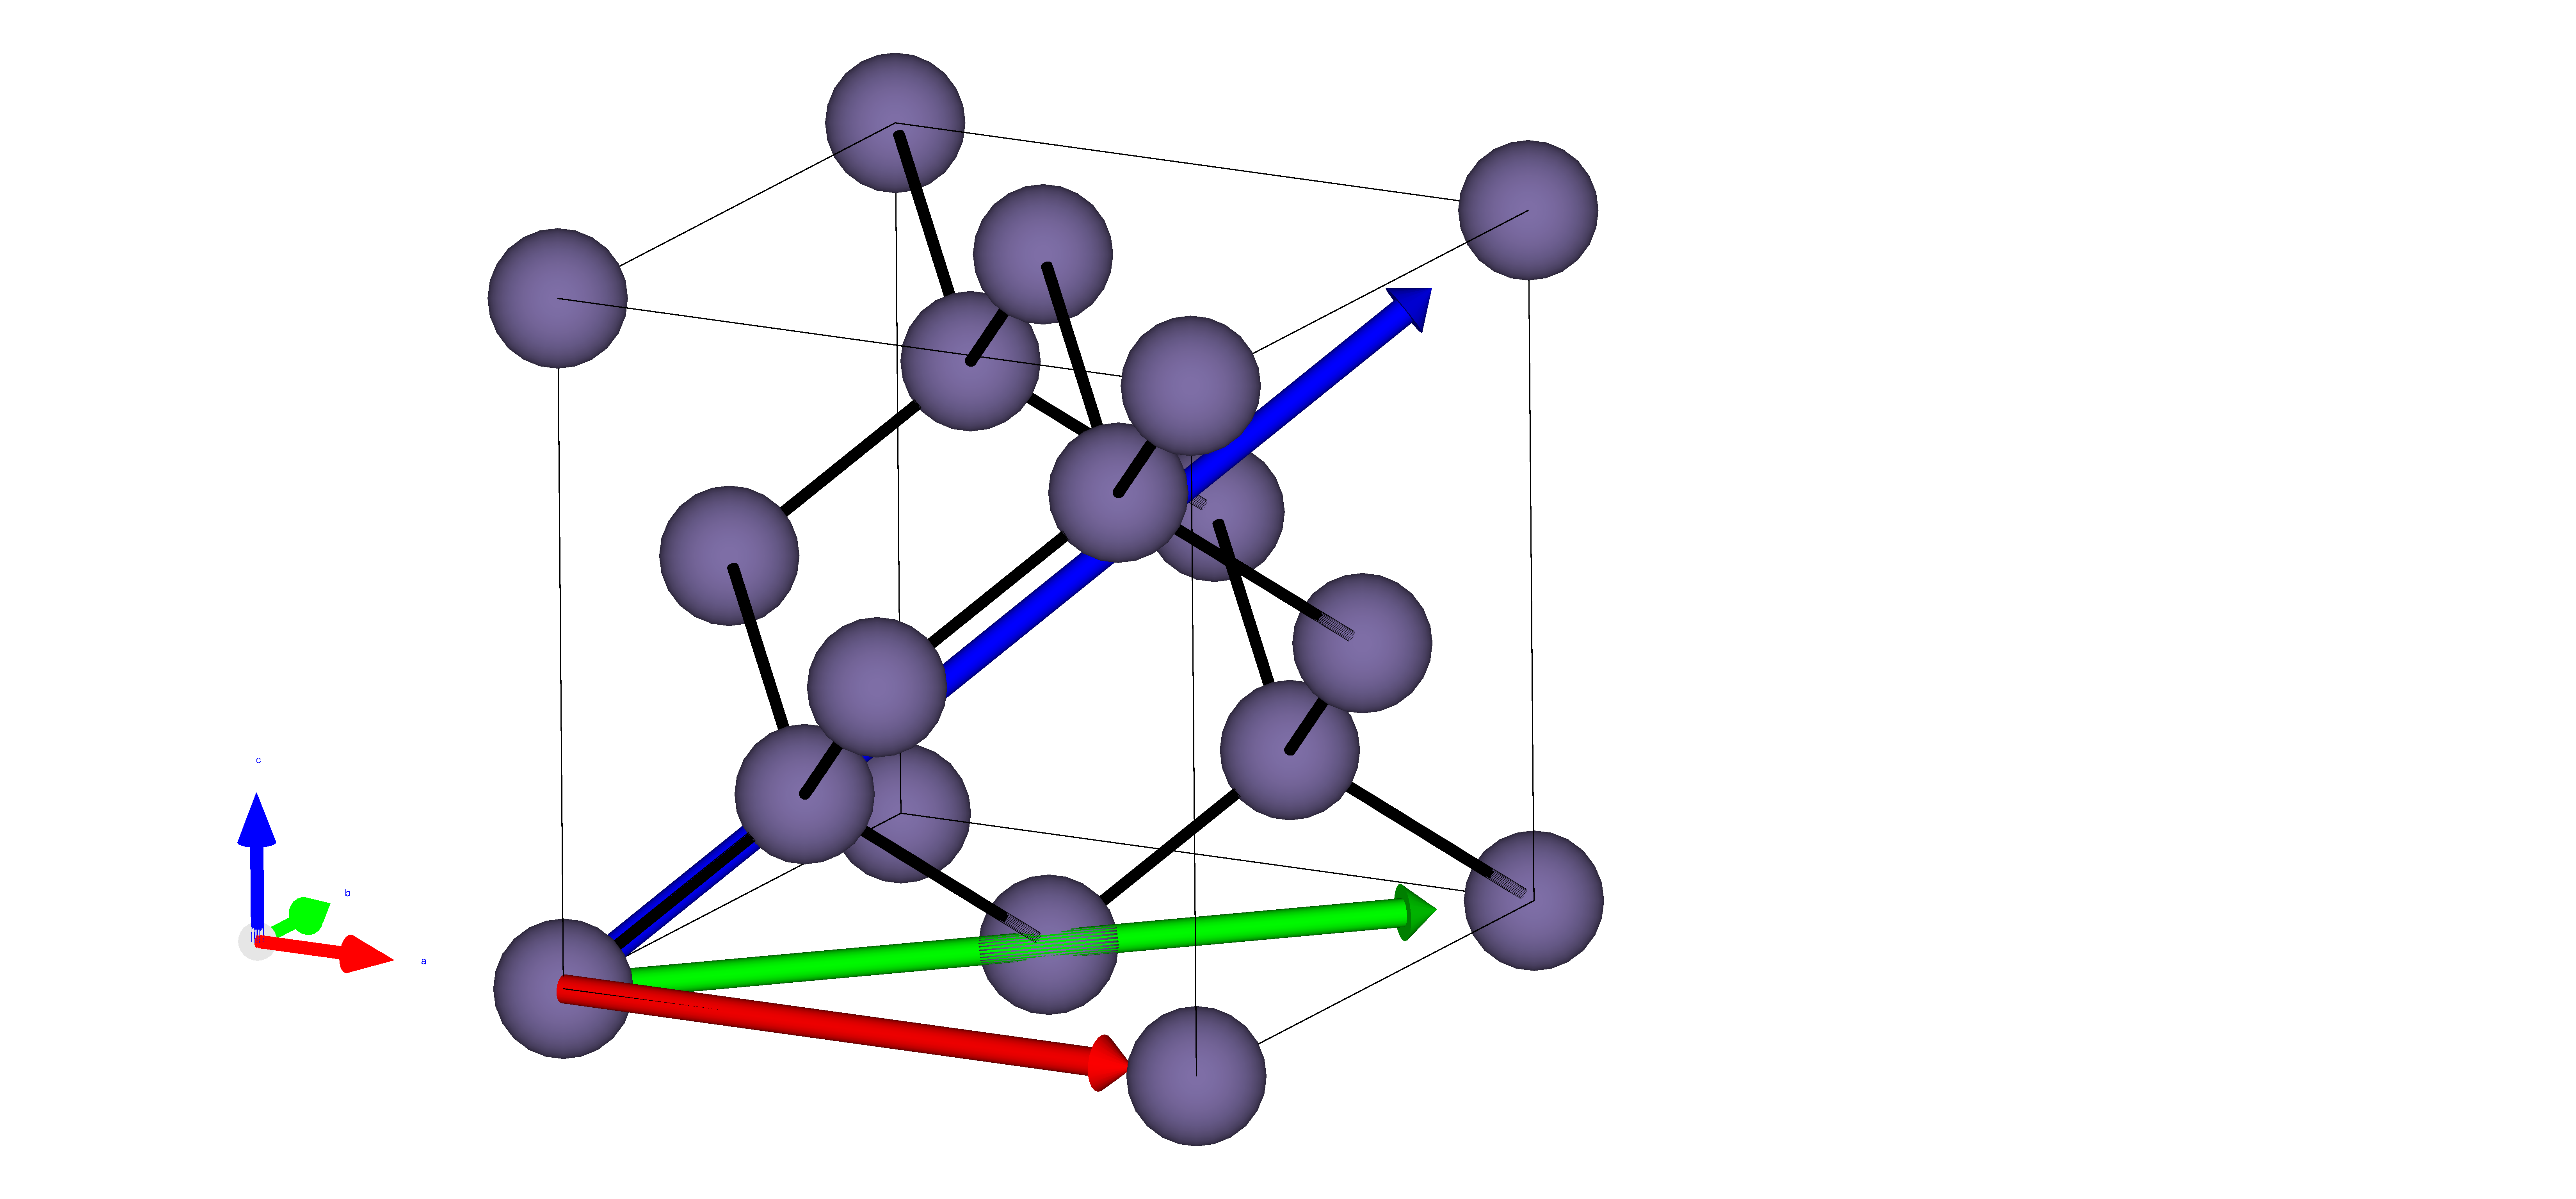
\includegraphics[width=1\textwidth]{strain/strain_direction.pdf}
	\caption{Relevant strain directions in diamond structure: \textcolor{red}{$[100]$}, \textcolor{green}{$[110]$}, \textcolor{blue}{$[111]$}.}
	\label{Fig:strain_direction}
\end{figure}

After defining strain types, the range of staining must be set as well. In the literature, many articles can be found, both experimental and theoretical, concerning strains and their effects on electronic properties \cite{strain-limit1,strain-limit2,strain-limit3}.
Both compressive and tensile strains are investigated, usually in the range of maximum $4\sim5\%$ of equilibrium lattice constants.
Due to practical issues and technological limitations, the range of research conducted is up to $4\%$.
From now on, there will be used such a convention that: the tensile strains will be represented by positive numbers, while compressive ones with negative.
Although of main interest was the effect of strain on electronic structure the investigation began with studying the structural properties, i.e. the effect of axial and biaxial strain on lattice parameters and atomic positions.

At first, for every system, the lattice represented by \prim\ were optimized and equilibrium lattice parameter were established.
Then the negative and positive isotropic strain was applied by elongating/shortening the lattice parameter, and respective stress (pressure in this case) was found.
In the next step, the response to biaxial and axial strain with respect to directions $[100]$, $[110]$ and $[111]$ was evaluated.
The optimization algorithm has difficulties with atomic positions improvement in \prim, due to lack of atoms to interact with.
For that purpose the appropriate supercells were constructed, strains were applied, the remaining structural degrees of freedom (the lattice and atomic ones) were optimized, and the induced stress was evaluated.

Supercells are a stack of crystallographic cells, in certain or multiple directions, that are built usually to optimize atomic structure, create alloys and admixtures (periodic boundary conditions), or add defects to structure, or simulate surface effects.
Those made for diamond structure calculations are shown on figure \ref{Fig:supercells}.

\begin{figure}[!htbp]
	\centering
	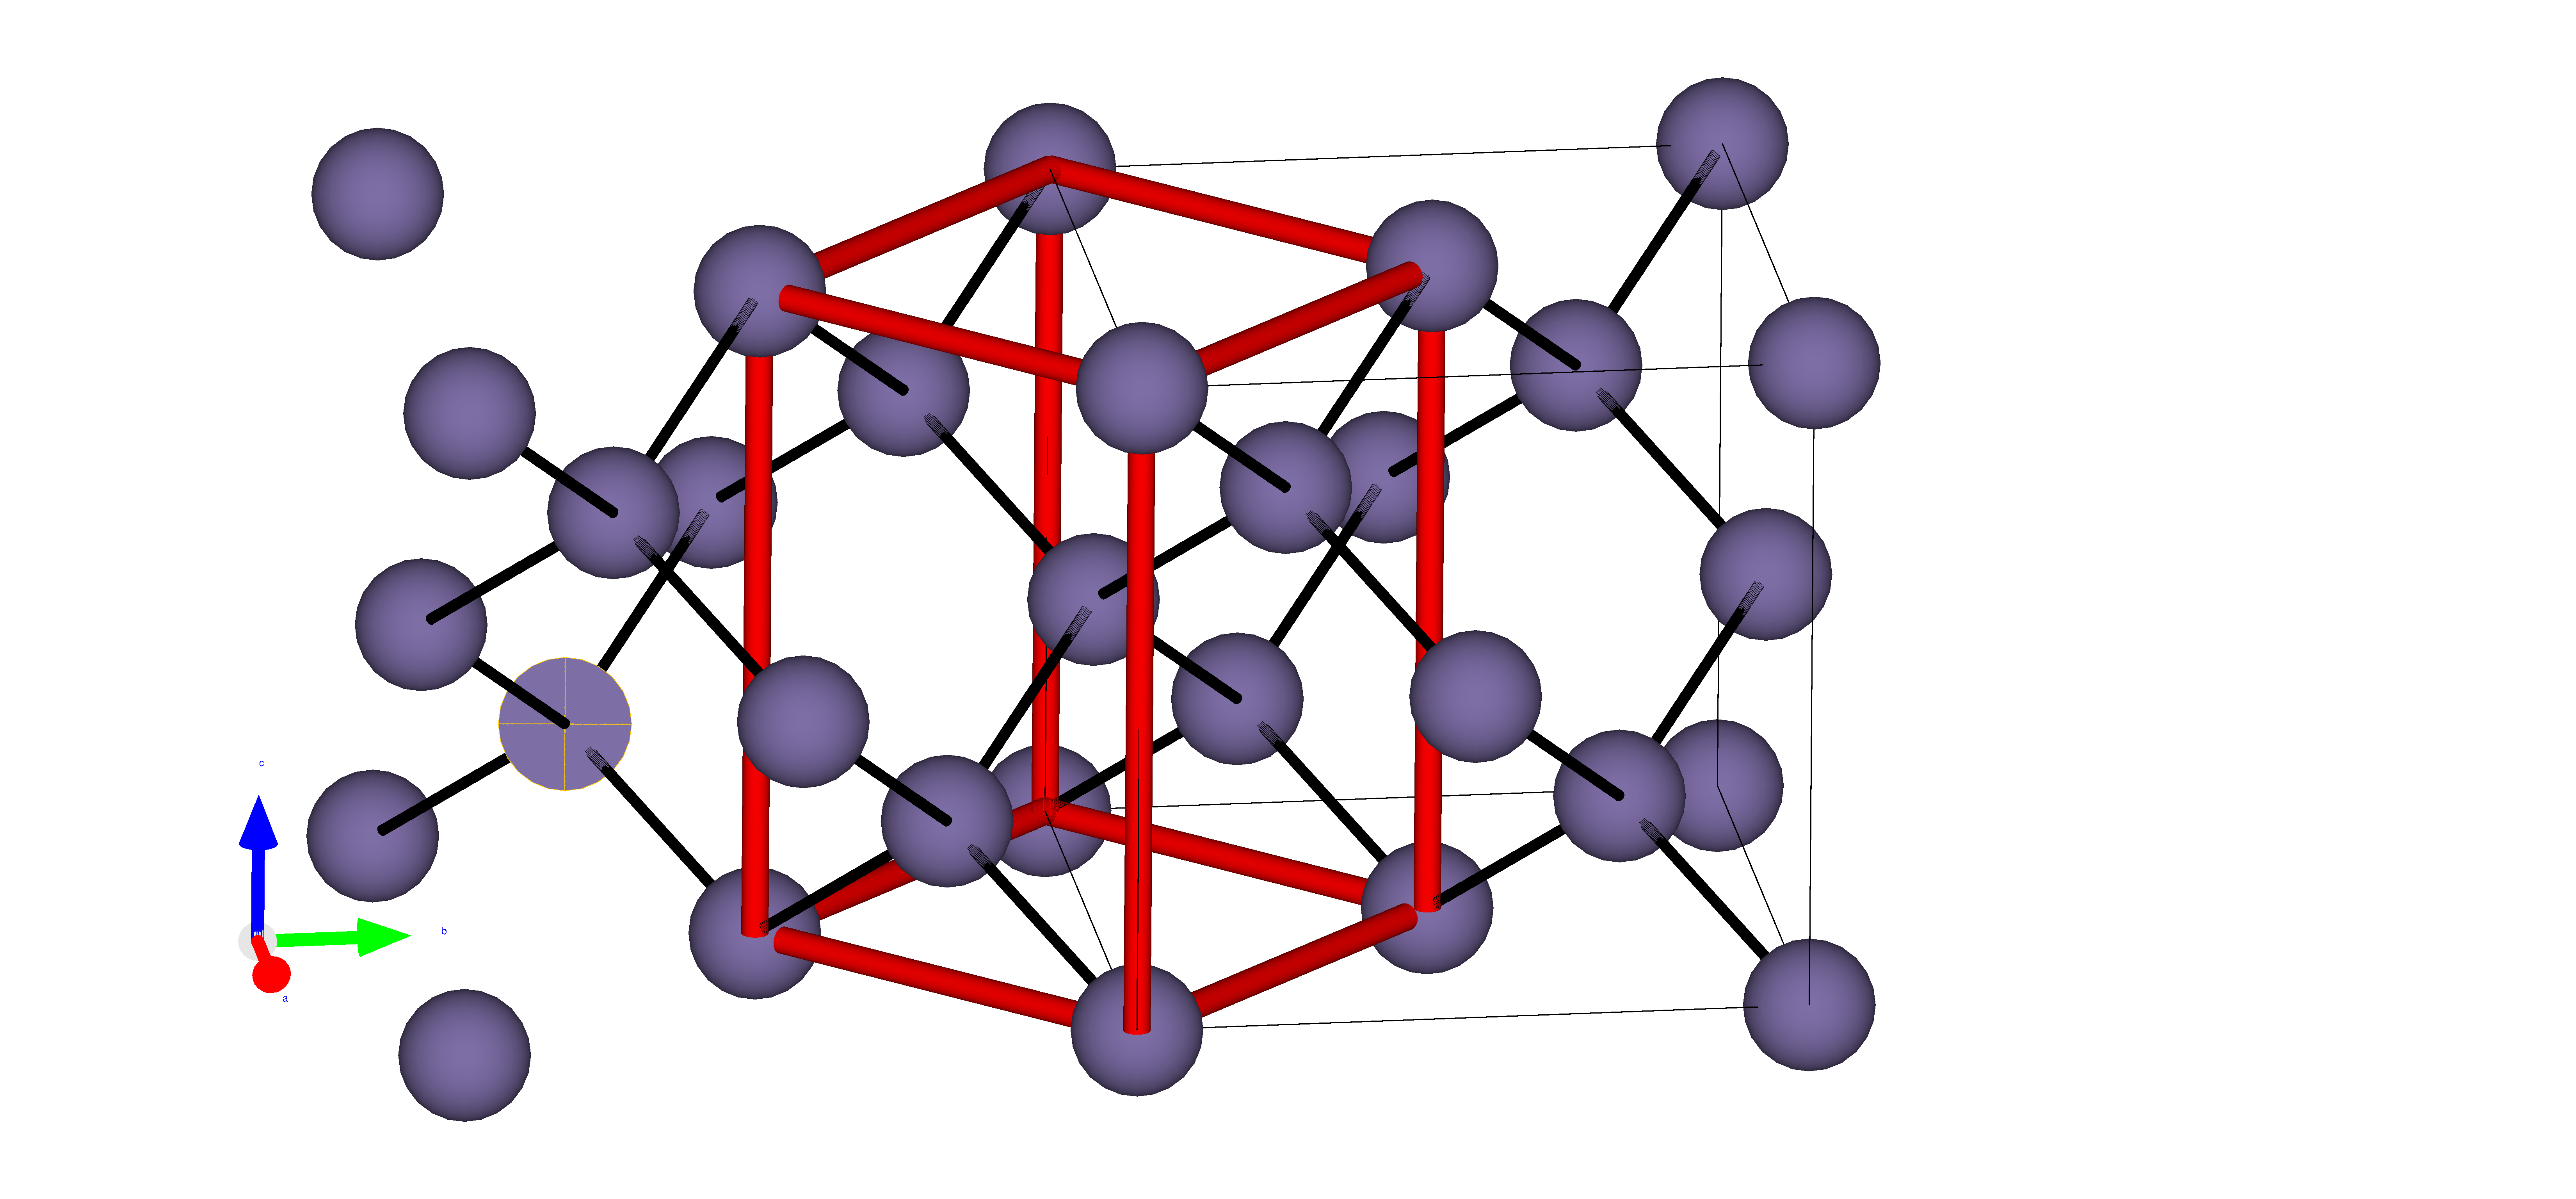
\includegraphics[width=.8\textwidth]{strain/100_supercell.pdf}
	\caption{Supercell for optimization in [100] and [110] strain directions.}
	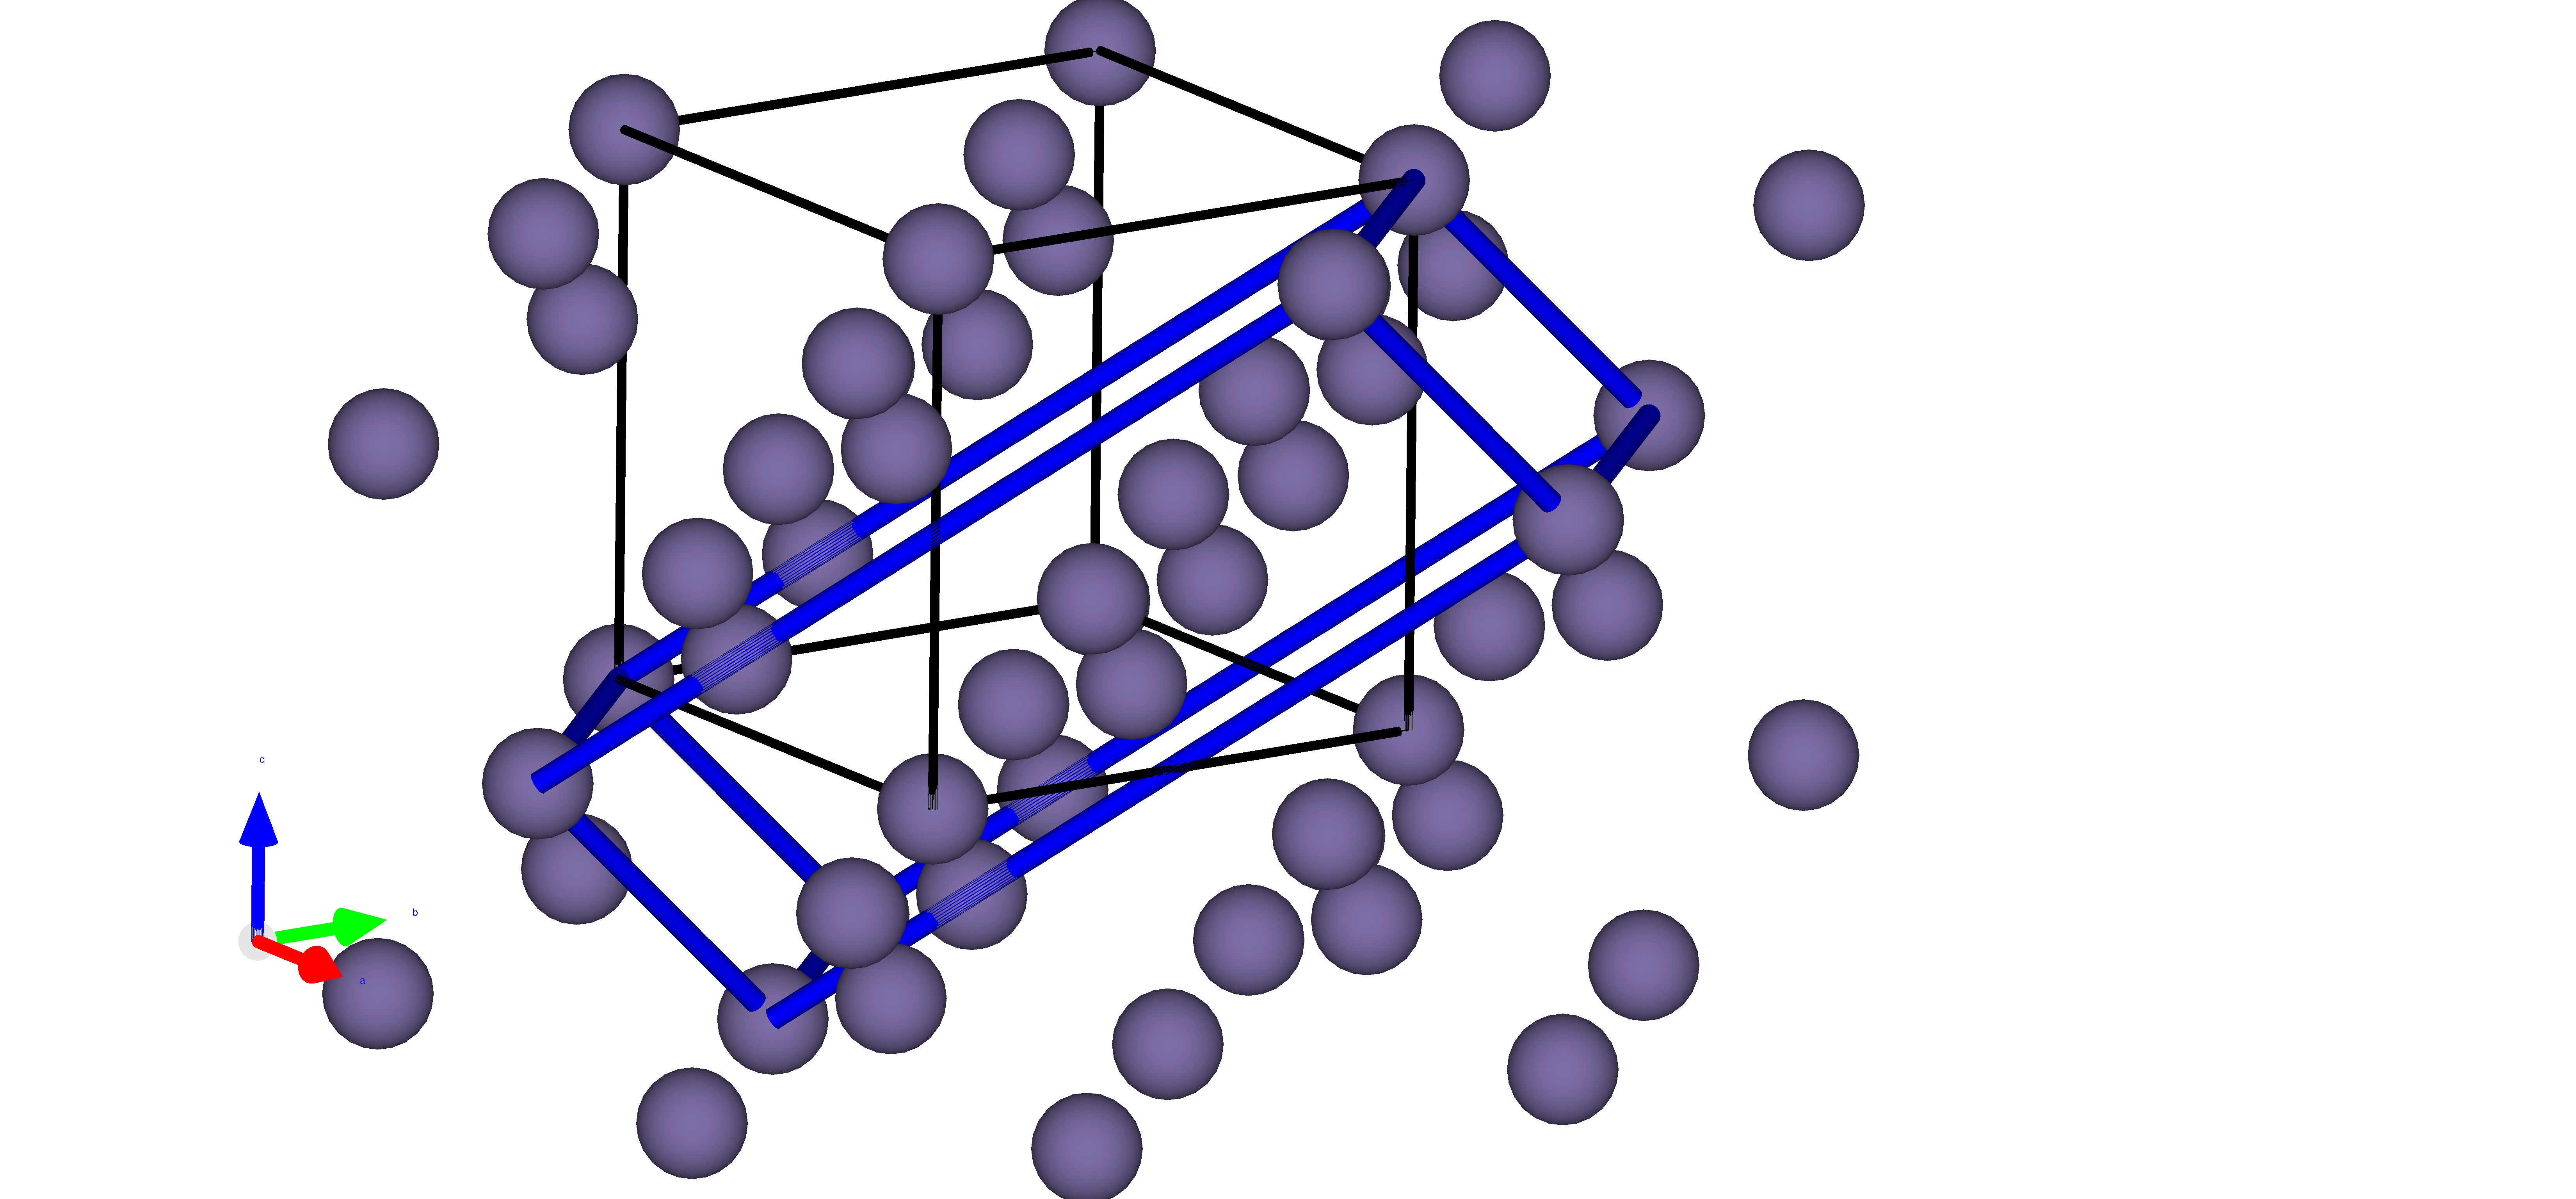
\includegraphics[width=.8\textwidth]{strain/111_supercell.pdf}
	\caption{Supercell for optimization in [111] strain direction.}
	\label{Fig:supercells}
\end{figure}

While constructing supercell it is crucial to remember what direction of strains will be applied.
In case of ABINIT package, during non--isotropic relaxation of cell shape, at least one lattice vector must be orthogonal to the remaining two.
Moreover, crystallographic directions, in which strain must be induced, must lay along lattice vectors.
Only then chosen direction dimension may be fixed.
Obviously, in case of planar strains, there is no need for that, as long as plane of strains is parallel to a plane spread on two of the lattice vectors.
Due to that, and the fact that the diamond structure has cubic symmetry, it was possible to construct one supercell for both $[100]$ and $[110]$ directions of strain.
Unit cell for $[111]$ direction was not obvious to construct.
One lattice vector must follow diagonal of the conventional cell.
As for the rest, nearest neighbours to $(0,0,0)$ atom in perpendicular plane to diagonal had to be found.
This led to hexagonal symmetry cell, of $120^\circ$ between non--diagonal lattice vectors.

Supercells constructed for applying strain in $[100$ and $[110]$ directions, and it's lattice vectors $a_1'$, $a_2'$ and $a_3'$, can be described by transformation matrix from conventional cell as

\begin{equation}
\label{Eq:trans_100}
\begin{bmatrix}
a_1' \\ a_2' \\ a_3'
\end{bmatrix}=
\begin{bmatrix}
0.5 & 0.5 & 0 \\
-0.5 & 0.5 & 0 \\
0 & 0 & 1
\end{bmatrix}
\begin{bmatrix}
a_1 \\ a_2 \\ a_3
\end{bmatrix},
\end{equation}

while for [111] as

\begin{equation}
\label{Eq:trans_111}
\begin{bmatrix}
a_1' \\ a_2' \\ a_3'
\end{bmatrix}=
\begin{bmatrix}
0.5 & 0 & 0.5 \\
-0.5 & -0.5 & 0 \\
-1 & 1 & 1
\end{bmatrix}
\begin{bmatrix}
a_1 \\ a_2 \\ a_3
\end{bmatrix}.
\end{equation}

All strains were applied in the range between $-4\%$ and $4\%$ of frozen respective lattice parameters and the structures were optimized without symmetries imposed (except identity) to avoid symmetry induced fixing of atomic positions.
To characterize the structural changes, the Poisson's ratio was used, defined both for the axial and biaxial strains as:

\begin{equation}
\label{Eq:poisson}
\poisson=-\frac{\epsopt}{\epsind},
\end{equation}

where $\epsind$, $\epsopt$ are respectively induced and optimized relative changes in a linear dimension along the considered direction and in the plane perpendicular to it. It should be mentioned that the isotropic behavior of a system around chosen axis takes place only for $[100]$ and $[111]$ directions.
For $[110]$ the Poisson's ratio defined above is not a well established quantity since under axial strain the relative expansion/contraction is not uniform around the axis and is the highest for $[001]$  and the lowest for $[1\bar{1}0]$.
Similarly, a uniform strain around $[110]$ axis leads to non-uniform stress.
Nevertheless, the $[110]$ direction has also been considered, with plane degrees of freedom naturally optimized under axial strain and biaxial strain applied uniformly, which may take place if a substrate in epitaxial technology is $(110)$ surface of a cubic symmetry crystal.
It is worth mentioning here that, from the definition, Poisson's ratio is defined for uniaxial strain, and falls within the range of $0-0.5$.
To be able to compare results from uniaxial and biaxial strain types, pseudo--Poisson's ratios ware also calculated for biaxially strained systems (later also called Poisson's ratio).

The resulting stresses ($\stress$) appearing at induced strains are described by respective elastic constants, first ($C1$) and second order ($C2$), so that the stress is given by the formula:

\begin{equation}
\label{Eq:stress}
\sigma=\text{C1}\cdot \epsind+\text{C2}\cdot \epsind^2.
\end{equation}

In the above formula $\epsind$ is a fractional relative change of a given dimension and the constants $C1$ and $C2$ are expressed in $GPa$. For the case of $[110]$ uniform biaxial strain there are two values of $C1$ and $C2$, corresponding to $[001]$ and $[1\bar{1}0]$ directions.
It should be noted that the elastic constants defined above are not directly related to standard elastic matrix elements.
However, for verification purposes the standard elastic constants have been derived from presented results and compared with the textbook data.
In the case of cubic symmetry there are only three non-zero and independent elastic constants ($c_{11}$, $c_{12}$, $c_{44}$).
All of them have been calculated from $C1$ and $C2$ values via standard transformation rules of stress tensor.
\footnote{Derivation of elastic constants from obtained results can be found in appendix \ref{chap:derivations_stress}}
Because of small differences in results for different strain directions, the average values and standard deviations are given in part \hyperref[part:III]{\Romanbar{III}}.

In the next step, the electronic structure was studied.
Supercells are inconvenient for band structure analysis, due to their sizes which, on the other hand, change volume or even shape of \BZ.
That makes it difficult to find meaningful points in \BZ\ and moreover causes problems with folding of bands.
To avoid the problems in supercells mentioned before, they have been transformed back to \prim.
The detailed derivation of transformation is described in appendix \ref{chap:derivations_supercell}.
Owing to such an approach the changes in the electronic band structure could have been easily followed since the relative positions of characteristic points in the deformed by strain \BZ\ remained unchanged with respect to the equilibrium state \BZ.
Of the main focus were characteristic energy gaps between \VB\ and \CB, $\Gamma$--$\Gamma$ (direct band gap), $\Gamma$ -- minimum along $\Delta$ directions and $\Gamma$ -- minimum along $\Lambda$.
The expected splitting of energies within $\Delta$ and  $\Lambda$ stars caused by symmetry breaking can be observed.
In the case of strained systems, where there is a lack of experimental data, the \textit{c} parameter (Eq. 3 in \cite{mBJLDA}) (responsible for the band gap value) was set as follows
\begin{equation}
\text{c}^{st}=\text{c}^{st}_{sc}\cdot\frac{\text{c}^{eq}_{fit}}{\text{c}^{eq}_{sc}},
\label{Eq:ctbo9}
\end{equation}
where \textit{st} means strained, \textit{eq} -- equilibrium, \textit{fit} -- fit to experiment, \textit{sc} -- \SC\ value.

At this point also the effective masses have been evaluated as functions of strains.
The calculations of effective masses were performed by fitting the 3rd order polynomial, which was necessary because of asymmetry of the bands around minima.
For the sake of reliability, $5$ to $9$ points around band extrema were taken into consideration, and the densities of points along k-space path were subjected to convergence studies.
In the \CB\ the effective masses at $\Gamma$ point as well as at the valleys along $\Gamma$-$X$ and $\Gamma$-$L$ directions have been calculated, taking into account also the star-degeneracy removal due to the broken symmetry under strain.
In the \VB\ only the top of the band at $\Gamma$ point has been considered, whether it was the heavy or the light hole band (due to inversion of bands).
The effective masses were evaluated from the inversion of the second derivative of fitted polynomial at the extremum.

From quantum mechanics, it is known that, all of the physical observable's changes are smooth.
Which means that non--smooth behaviour must be investigated further.
To better understand non--smoothness appearing in band structure, it is worth to calculate the orbital composition of bands.
In practice it projects band structure on each orbital of every atom in the system allowing to look into symmetry of certain band and trace it's movement along with straining.
Two most common physical effects that usually occur are: band inversion and splitting of bands.
First one happens when bands degenerate, e.g. when band gap closes.
Then former \CB\ moves beneath former \VB.
Second effect may occur during symmetry break.
While breaking the symmetry of the system, usually (depending on actual space group), especially \VB, band might loose it's degeneracy, resulting in splitting.

In the last step, the deformation potentials $a_v$, $a^{dir}$, $a^{ind}$ $b$, $d$, $\Xi_u^{\Delta}$, $\Xi_u^{L}$, as defined in \cite{pot-def} were calculated.
In the calculations of $a_v$, $b$, and $d$, which are absolute in the sense that they describe the changes in absolute positions of some points in bands, the crucial point is to establish the unified energy reference point, i.e. the reference point which do not flow with the strain.
For that purpose we have used the natural slab method \cite{zunger} in which we assume that the energy level in vacuum should not change under strain, and thus defines the energy reference point.
There are also a few rules one should keep in mind preparing the calculations:
\begin{itemize}
    \item for both slab and bulk calculations, it is crucial to set the same k--point grid.
    In a slab a good practice is to adjust number of k--points to slab size.
    E.g. In bulk set k--points to $10\times 10\times 10$, while slab in $[100]$ direction of $5$ layers of material and $5$--layer--long vacuum set to $10\times 10\times 1$.
    That way slab layer and bulk have exactly the same k--points distribution.
    \item vacuum must be long enough for the plateau to be clearly visible.
    the flat area should be wide enough for a small fluctuation to emerge.
    That guarantees the vacuum to clear of slab potential.
\end{itemize}

\begin{figure}
	\centering
	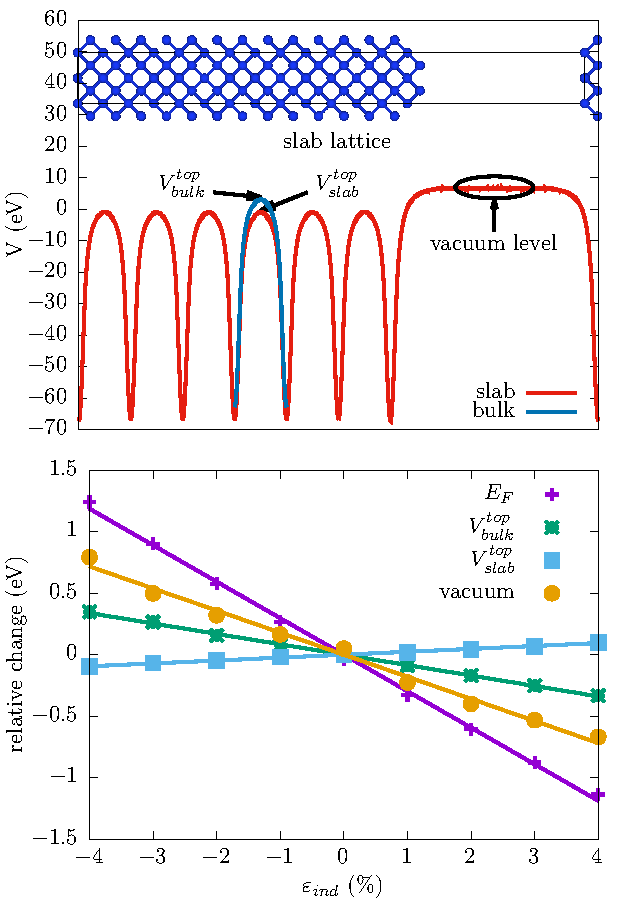
\includegraphics[width=1\textwidth]{strain/offsets.pdf}
	\caption{Illustration to the deformation potential determination procedure, for Si under isotropic strain. Upper figure: the lattice used and the \SC\ potential throughout this lattice (red line) as well as corresponding potential in bulk (blue line). Lower graph, the strain induced energy variations necessary to evaluate the deformation potential.}
	\label{Fig:offsets}
\end{figure}

Figure \ref{Fig:offsets} illustrates where the partial data are taken from in the calculations of $a_v$ in Si under isotropic strain.
To establish the unified energy reference point we apply the following assumptions: i) the vacuum level should not change under strain, ii) The rates of the changes in the \SC\ potentials at chosen point in bulk and equivalent point in the slab, under strain, should be the same.
Thus, when defining the linear coefficient of lines in Fig. \ref{Fig:offsets}: $a^F$ - \VBM, $a^{Vb}$ - \SC\ potential value at chosen point in bulk (maximum), $a^{Vb}$ - \SC\ potential potential value at equivalent point in the slab, $a^{Evac}$ - energy level in vacuum, the deformation potential $a_v$ can be calculated from the formula:

\begin{equation}
\label{Eq:av}
a_v=(a^F - a^{Vb} + a^{Vs} - a^{Evac})\cdot100/3,
\end{equation}

where the factor $100/3$ comes from the transformation from percent to fraction, and from linear to volume change.

The corresponding uncertainties have been calculated from linear coefficients uncertainties in \abinitio\ data approximations, assuming the ''worst case'': 

\begin{equation}
\label{Eq:Dav}
\Delta(a_v)=[\Delta(a^F) + \Delta(a^{Vb}) + \Delta(a^{Vs}) + \Delta(a^{Evac})]\cdot100/3.
\end{equation}

The described procedure was used in the calculations of all the absolute deformation potentials.
In the calculation of relative deformation potentials $a^{dir}$, $\Xi_u^{\Delta}$, $\Xi_u^{L}$ the procedure is not necessary because when calculating the energy differences (e.g. $E_c-E_v$) the subtracted energies are always given with respect to the same energy reference point.

Thus, in the calculations the same supercell as for the $[100]$ and $[110]$ structure optimizations have been used except a vacuum layer has been added, i.e.  $3-4$ layers of optimized supercell and $6-7$ supercell--layers--long distance of vacuum.
The total potential across the whole supercell (in the direction perpendicular to the slab) was evaluated for slabs with and without separating vacuum layer.
As a result the energy variation slopes described above were found, corresponding to respective deformation potentials.

\ornament

\section{Alloying}
\label{sect:alloy_theory}

In this part of work all calculations were performed with ABINIT software package.

Second presented method of band structure engineering is alloying.
Creating alloys and admixtures of different materials (even slightly) can drastically change materials properties, especially in case of semiconductors, which are known for their huge sensitivity for impurities.
Main difference between alloying and doping is percentage of admixture.
It is worth noting that low (light) doping is considered to be, when one dopant atom is added per 100 million atoms, while heavy (high) doping per ten thousand atoms.
Alloy, on the other hand, is concerned when admixture is per one hundred atoms and less.

In case of silicon technology impurities are usually added in bulk growth process.
Proper application of this technique provides nearly uniform impurities doping in each silicon wafer.
Also through photolithography, the process of doping selected areas can be conducted by diffusion and ion implantation (high control over the process).

Before getting further into band structure engineering it should be stated what within this thesis 'alloy' actually means.
The concept of alloy is quite vast and covers many different material types.
From uniform materials to multi--phase ones, including all types of doping in atomic scale.
A doping atom can substitute base atom, create vacancy or fit in interatomic position.
That gives large field of study, too big actually to cover all this cases in research.
Thus some choice has been made.
In this work only uniform phase with substituting base atom is taken under consideration.

The active region of modern optoelectronic devices (detectors, light emitting diodes, lasers, etc.) is often based on semiconductor alloys.
They offer an opportunity of tuning the band gap by varying their composition.
One of materials of interest in the field is the $\mathrm{Ge_{1-x}Sn_x}$ alloy \cite{homewood15, shigeaki15, margetis17, jeremie19, tran19}.
Its direct gap can be tuned in the range of $0.89-0$ eV by varying the composition \cite{growth,sigesn, Polak_2017, zhao20}.
Additionally, it exhibits an interesting property, where by varying the alloy composition, a transition from indirect to direct band gap is possible.
This transition appears at a relatively small admixture of Sn in Ge (around $6.5\%$) (e.g. \cite{Polak_2017}).
This feature, joined with the observed high mobility of carriers, makes this material a promising candidate for optoelectronic applications.
This fact has been a reason for an extensive experimental and theoretical investigations of this material, e.g. \cite{sigesn, Polak_2017, snge, zhao20,growth,PhysRevLett.79.1937,gesn-engineering,vegard,sisnge,gesn-0.14,ge_alloy_compare,electroreflectance, random_alloys,doi:10.1063/1.125558,SAHNOUN2005392,Moontragoon_2007,PhysRevB.78.161203,small_sn,ZHANG201212,article,doi:10.1063/1.4790362,HUANG201443,PhysRevB.89.165201,coherent_approx,C5CP02558C}.
In particular a number of \DFT\ based \abinitio\ theoretical studies have been conducted \cite{Polak_2017, zhao20, snge, random_alloys,doi:10.1063/1.125558,SAHNOUN2005392,Moontragoon_2007,PhysRevB.78.161203,small_sn,ZHANG201212,article,doi:10.1063/1.4790362,HUANG201443,PhysRevB.89.165201,coherent_approx,C5CP02558C}.
It is a known fact that the \abinitio\ methods provide very realistic predictions of properties of atomic systems but often at a high computational costs.
In the case of alloys, the method of choice is the use of periodically repeated supercells containing up to a few hundred of randomly distributed atoms of species forming the system, which makes the calculations computationally time consuming \cite{PhysRevB.89.165201,coherent_approx,C5CP02558C,Polak_2017}.
The most prominent advantage of this method is the ability to include lattice distortion around impurities, as well as vacancies in the structure and even interatomic position dopants.
Although, in such approach only a discrete number of compositions can be analyzed.
Also, the problem emerges in choice of atoms substituted in whole supercell, such that it would statistically represent the best bulk material.
For that purpose \SQS\ (Special Qausirandom Structures) \cite{sqs} are usually used.
Although, it should be kept in mind that they only increase the chance to statistically well represent the material.
More important is appropriate size of supercell.
Moreover, the use of large supercells results in numerous folded bands which makes the interpretation of the picture of the band structure rather complicated.
The necessary unfolding procedure \cite{unfolding} provides an effective band structure represented in the form of spectrally weighted eigenvalues, which are the more torn and blurred the more percentage of admixture.
That makes their direct application in modeling of semiconductor devices very inconvenient, due to often large blur of bands.
For this reason, in device modeling other representations of electronic bands are most often used, among which the $\mathbf{k}\cdot\mathbf{p}$ method seems to be the most popular \cite{richard05, kurdi10, gladysiewicz13, gladysiewicz14, maczko19}.
These methods require certain number of parameters which are found from fitting either to experimental data or to large scale \abinitio\ calculations.

For this task is applied an approach which joins large scale \abinitio\ calculations with 30-band $\mathbf{k}\cdot\mathbf{p}$ method, which is known to correctly reproduce the electronic band structure in the full \BZ.
This approach allows to find the values of the parameters used in the $\mathbf{k}\cdot\mathbf{p}$ method.
Finding them directly from \abinitio\ supercell data would be difficult (if possible at all), due to the character of the obtained band structures.
Therefore, it is proposed to make an intermediate step which is based on other \abinitio\ approaches.

Despite supercell method there are basically three more methods suitable for alloy calculations.
First one, and the simplest, is Virtual Crystal Approximation \cite{vca1} (\VCA).
In practice, each site occupied by more than one different atom type is set with virtual atom interpolating behaviour of site components.
By that, it ignores all short range interactions around disordered site, what follows possible local lattice distortion.
The advantage of this method is low computational cost, of the order of ordered structures.
Either way, \VCA\ was useful enough to be modified in various manners, suitable for specific group of materials \cite{vca_mod1,vca_mod2}.
Second approach is so--called Coherent Potential Approximation (\CPA).
It is physically the most sophisticated method, as it is supposed to model scattering properties of disordered system.
This approach is appropriate for Green's function formalism, in which \KKR\ method is implemented.
Unlike \VCA, the \CPA\ instead of mixing potentials and creating average atom, it mixes Green's function of whole system with all of the components separately.
Moreover in different combinations (if the site has more equivalent positions).
That way, it  approximates a configurationally random alloy with an effective medium that is determined self-consistently from the condition of stationary scattering.
On the other hand, it is insufficient for geometry optimisation or total energy calculations.
Due to that, impurities which highly distort lattice will not be well represented.
Third method available is Computational Alchemy.
This one bases on perturbation theory to calculate the response to the difference of \VCA\ potential and the real one.
One can treat this approach simply as a correction to \VCA.

Because \CPA\ method requires Green's function approach and as output gives Bloch's spectral function instead of typical band structure, that method also was rejected for device modeling purpose.
\VCA\ on the other hand is not accurate enough method due to its simplicity.
Thus a computational alchemy was chosen, as a more reliable technique than \VCA\ and applicable unlike \CPA\ and supercell calculations.

The approach has already been exploited in a number of works, e.g. \cite{ingap_alch,gesi_mc_alch,alloys_alch,vca}.
The ABINIT package was used with implementation of the computational alchemy, called the Alchemical Mixing (\AM).
The \AM\ itself is known to provide rather poor description of electronic structure, particularly for highly mismatched alloys (\HMA), mainly because it does not account for the local distortions of the lattice \cite{ingan}.
However, when used as a model containing additional fitting parameters it is able to accurately reproduce the band structure for any composition of an alloy at low computational costs.
Thus, at the first step, the \AM\ method is used to approximate the reference supercell unfolded band structures.
Next, the continuous \AM\ bands are used to find the values of the parameters of 30-band $\mathbf{k}\cdot\mathbf{p}$ model, through a specially designed optimization method.
As a result, an effective full \BZ\ electronic band structure description of the $\mathrm{Ge_{1-x}Sn_x}$ alloy in the full composition range is obtained.

As mentioned above, to approximate the \abinitio\ supercell band structure we the concept of computational alchemy has been used, as implemented in the ABINIT code \cite{abinit1} and called the alchemical mixing (\AM) there.
The idea is similar to the \VCA\ \cite{vca}, often used to describe mixed crystals within empirical potential approach.
In the \AM\ approach a scattering center (ion) is created whose properties reflect the properties of two ions simultaneously, at a given proportion.
The \VCA\ relies simply on a linear combination of two one-electron potentials of parent compounds.
The alchemical mixing of pseudopotentials implemented in the ABINIT package uses the following construction \cite{abinit2}:
\begin{itemize}
    \item the local potentials are mixed in the proportion given by mixing coefficients,
    \item the form factors of the non-local projectors are all preserved,
    \item the scalar coefficients of the non-local projectors are multiplied by the proportion of the corresponding type of atom,
    \item the characteristic radius of the core charge is a linear combination of the characteristic radii of the core charges,
    \item the core charge function $f(r/rc)$ is a linear combination of the core charge functions.
\end{itemize}

In all the linear combinations the mixing coefficients reflect the proportion at which particular atoms enter the alloy are used.
In the approach only the atoms with the same valence electronic configuration can be taken (isovalent elements, like e.g. Ge and Sn).
In this work the Hartwigsen-Goedecker-Hutter (\HGH) pseudopotentials \cite{hgh} have been used.

There is a lot of freedom in choosing the mixing proportions, the only constrains are that the overall formula $\mathrm{Ge_{1-x}Sn_x}$ must be fulfilled at every composition, and that the content of an element in an \emph{alchemical} atom must not be negative.
There has been used a scheme which, on the one hand, guarantees a consistency of mixing for any composition and, on the other hand, allows, in some extent, to check the effect of mixing proportions on the results.
The two \emph{alchemical} atoms representing two sublattices in \BZ\ structure, $A1$ and $A2$, are composed from Ge and Sn atoms according to the formulas:

\begin{align}
\label{Eq:mixing}
\begin{split}
A1=Ge[(1-x)+\alpha x(1-x)] + Sn[(x)-\alpha x(1-x)]\\
A2=Ge[(1-x)-\alpha x(1-x)] + Sn[(x)+\alpha x(1-x)]
\end{split}
\end{align}
where $\alpha$ is a parameter responsible for the proportion of mixing and can be varied in the range $[0,1]$.
The mixing parameter $\alpha$, if non--zero, allows to add a bowing to the mixing curve versus the amount of admixture, and what follows, to not equally occupy chosen site by component atoms.
Testing it's impact on results is vary important.
Value of $\alpha$ resembles the arrangement of atoms in supercell.
What follows, in larger cells with higher number of independent sites, the obtained results can be sensitive to the choice of mixing parameter.

One of the advantages of the \AM\ approach is a significant reduction of system size to be analyzed from first principles, which can be reduced to a \prim.
However, the accuracy of such approach is questionable, in particular it does not account for the local distortions of the lattice \cite{ingan}, which is significant in \HMA s where the local relaxation effects play a crucial role \cite{Polak_2015}.
Nevertheless, the \AM\ approximation, when used together with supercell calculations \cite{Polak_2017} as reference, can be very useful.
When properly adjusted to the supercell data, they may provide a very good approximation of electronic bands with continuous curves.
Therefore, there was designed a procedure of utilizing the \AM\ approach in a way that allows to reproduce results obtained with more accurate methods, including supercell \DFT\ calculations and experimental measurements.
In this chapter is demonstrated the applicability of the method with results of \DFT\ supercell calculations serving as reference.

There are only two key parameters necessary to achieve realistic band gaps:
\begin{enumerate}
    \item lattice constant,
    \item $c$ parameter from \mBJLDA.
\end{enumerate}

Each provides different changes to band structure and must be considered with respect to the other one.
Usually, in case of semiconductors, direct and indirect band gaps are to be well modeled.
As it is shown in \ref{chap:strains}, manipulating lattice constant (compressing or stretching material isotropically) closes or opens band gaps.
Major visible effect is shift of whole bands.
Although it should be pointed out that changes between certain valleys on the same band will appear.
And for that second reason lattice constant is used.

On the other hand $c$ parameter in functional serves to manipulate distance between valence bands and conduction bands (which is the purpose of \mBJLDA\ functional).
Also this parameter changes ratio between direct and indirect band gap, due to bands flattening.
The effect is not strong but must be taken into consideration while increasing fitting accuracy.

As first lattice constants should be evaluated.
Due to fitting nature of this method, at the beginning must be found such constants that would give proper band gaps on boundary conditions.
In the case of $\mathrm{Ge}_x\mathrm{Sn}_{1-x}$ band gaps and and other necessary parameters (like $c$ parameter in \mBJLDA\ \ref{Eq:c_mbj}) can be taken from strain calculations.

After obtaining lattice constants with correct band gaps it is necessary to be able to achieve accurate constants for any alloy composition.
Usually for that purpose Vegard's law is applied \cite{vegard1}.
It states that the lattice constant for chosen alloy composition is linear combination of lattice constants of alloy composing materials equivalent to percentage of mixing.
It should be noted that there are many exceptions from Vegard's law \cite{vegard2,vegard3,vegard4}.
Such an exception is $\mathrm{Ge}_x\mathrm{Sn}_{1-x}$ as well \cite{Polak_2017}.
In lattice constant vs composition occurs visible bowing.
Due to that fact, to properly model the whole range of composition, another point on the curve or bowing parameter is necessary to duplicate supercell results.

While $\mathrm{Ge}_x\mathrm{Sn}_{1-x}$ does not obey Vegard's law, other materials usually obeying stated relation might still need to include a bowing.
The main goal is to accurately describe band gaps characteristics.
If material obeys Vegard's law but the \AM\ band gaps are inaccurate with real lattice parameters, there might be a need to manipulate lattice constant to achieve an agreement with experimental / supercell results.

What is left is a choice of searching algorithm.
There are only two parameters.
The easiest way (and maybe the most efficient one) is work on bowing parameters for lattice constant and $c$, instead of actual values.
That way, there is only a need to specify two variables to generate whole stack of calculations for each admixture amount, that experimental (or supercell) data are provided.

Having parameterized necessary variables, band structure calculations can be performed.
The procedure for that calculations, as well as estimating effective masses of charge carriers, is equal to strain research that was described previously (\ref{sect:alloy_theory}).

\ornament

\section{Structural factor}

In this part of work all calculations were conducted with VASP software package.

The third method of electronic structure engineering, mentioned in the introduction, is the formation of alternative (metastable) crystal structures.
Modern deposition technologies, like molecular beam epitaxy (MBE) or metal--organic chemical vapor deposition (MOCVD), open such opportunities.
Usually the structure is induced by the substrate (e.g. wurtzite structure by the (111) surface of zinc blende crystal).
In principle any crystal structure can be formed, but the most important issue is the stability and thermodynamic stability of the system.
It is a known fact that the diamond structure is the stable one for Si and Ge, however, for C itself (diamond) is a metastable structure, and although rather difficult to be formed it is a well known system and has various applications, in jewelery in particular,  but not only.
Diamond owing to its exceptional hardness, very high thermal conductivity (phonon induced), very good electrical insulation properties, transparency for light, has various applications in technics, e.g. diamond anvil cells for creating the high pressure environment.
This example shows, that the formation of metastable crystal structures is an open way in the band structure engineering.

In this work only the wurtzite structure will be taken into consideration, since it is energetically very close to the diamond one, and relatively easy to obtain, by deposition on the (111) zinc blende plane.
Some properties of such structures of Si and Ge are already known \cite{wz_si_exp1,wz_si_exp2,wz_si_exp3,wz_si_exp4,wz_si_exp5,wz_ge_exp6}, in particular it turns out that the fundamental band gap in Ge is direct, (unlike in the diamond structure) which is a crucial feature in optoelectronics.
It is worth mentioning that mostly Si was investigated, while Ge barely exists in the literature.
The available data range from achievement of Si wurtzite nanowires \cite{wz_si_exp1}, \abinitio\ studies of strained Si, through vibrational \cite{wz_si_exp2} and doping properties \cite{wz_si_exp3,wz_si_exp4}, up to Raman spectrum of Si \cite{wz_si_exp5}.
Apart from the formation energies, the elastic constants and the Poisson ratio, the systematic investigations of the effect of strains has been performed, for C, Si and Ge.
The isotropic (pressure), biaxial (perpendicular to c--axis) and axial (along c--axis) strains have been considered.
In particular the effect of strains on the band structure and its crucial features: band gaps (identification of fundamental gaps) and effective masses.
Such calculations have allowed also to evaluate the deformation potentials, crucial parameters in the calculations of superstructures electronic bands and of the electron--phonon coupling. 


For all of the calculations presented here, VASP \cite{vasp1,vasp2} software package was used, mainly due to implementation of \mBJLDA\ on \PAW\ pseudopotential.
The procedure was similar to the one presented in Chpt. \ref{chap:strains}.
Although, there are a few differences in methodology:
\begin{enumerate}
	\item The anisotropic strains are considered only with respect to one, [001] axis, which is typical when the structure is grown on (111) ZB substrate. The wurtzite cell is presented in Fig. \ref{Fig:wz_cell}.
	
	\begin{figure}[!htbp]
		\centering
		\includegraphics[width=0.7\textwidth]{/wurtzite/wz_cell2.pdf}
		\caption{Conventional cell of wurtzite (\#186).}
		\label{Fig:wz_cell}
	\end{figure}
	
	\item The conventional cell reflects the symmetry of the system, and its possible breaking in the case of anisotropic strains. In wurtzite structure the [001] strains do not lower the symmetry of the cell. What follows the \BZ\ stays the same, and no additional points must be observed. The \BZ\ of wurtzite is shown in Fig. \ref{Fig:wz_BZ}.
	
	\begin{figure}[!htbp]
		\centering
		\includegraphics[width=.6\textwidth]{/wurtzite/186.pdf}
		\caption{First Brillouin Zone of wurtzite crystal structure (\#186).}
		\label{Fig:wz_BZ}
	\end{figure}
	
	\item The differences in the formation energies between WZ and ZB structures is evaluated, to show the energetic preference. This also  gives some hints about stability, especially while straining the system. The thermodynamic stability remains still an open question which require  an independent investigations (lattice dynamics).
	
	\item In wurtzite materials two additional values seem to play important role as $\mathbf{k}\cdot\mathbf{p}$ parameters: the $\Delta_{so}$ and $\Delta_{cr}$. They are connected to \SO\ coupling and crystal field, and are known to be present in wurtzite crystals, and calculated as follows \cite{birpikus}:
	\begin{align}
		\Delta_{so} &= \frac{\Delta_1+\Delta_2}{2} - \frac{1}{2} \frac{c}{a^2}\cdot \sqrt{\Delta}  \\
		\Delta_{cr} &= \frac{\Delta_1+\Delta_2}{2} + \frac{1}{2} \frac{c}{a^2}\cdot \sqrt{\Delta}
	\end{align}
	where
	\begin{align}
		\Delta_1 &= \HH-\LH  \\
		\Delta_2 &= \HH-\CH  \\
		\Delta = \bigg(\frac{c}{a^2}\bigg)^{-2}\cdot (\Delta_1+\Delta_2&)^2-4\cdot\frac{a^2}{c}\big((\Delta_1+\Delta_2)^2-(\Delta_1-\Delta_2)^2\big)
	\end{align}
	
	\item Because of different symmetry compared to the diamond one the deformation potentials also differ as well as the way of calculating them. For wurtzite systems (including \SO) band structure deformation potential ($D_1$ to $D_6$) are defined by the equations \cite{birpikus}:
	\begin{align}
		\Delta E_1 &= E_1 - E_1^0 = (D_1 + D_3)\varepsilon_{zz} + (D_2 + D_4)(\varepsilon_{xx} + \varepsilon_{yy}) +\notag\\ &+\frac{D_6(E_1^0-E_2^0-E_3^0)(\varepsilon_{xz}^2+\varepsilon_{yz}^2)+D_5E_1^0[(\varepsilon_{xx}-\varepsilon_{yy})^2+4\varepsilon_{xy}^2]}{(E_1^0-E_2^0)(E_1^0-E_3^0)},\label{Eq:wz_def1}\\
		\Delta E_2 &= E_2 - E_2^0 = (D_1 + D_3\frac{E_2^0}{E_2^0-E_3^0})\varepsilon_{zz} + \notag\\
		&+(D_2 + D_4\frac{E_2^0}{E_2^0-E_3^0})(\varepsilon_{xx} + \varepsilon_{yy}) + \frac{E_2^0E_3^0}{(E_2^0-E_3^0)^3}(D_3\varepsilon_{zz}+D_4(\varepsilon_{xx}+\varepsilon_{yy}))^2 +\notag\\
		&+\frac{D_6(E_1^0-E_2^0+E_3^0)(\varepsilon_{xz}^2+\varepsilon_{yz}^2)-D_5E_2^0[(\varepsilon_{xx}-\varepsilon_{yy})^2+4\varepsilon_{xy}^2]}{(E_1^0-E_2^0)(E_2^0-E_3^0)},\label{Eq:wz_def2}\\
		\Delta E_3 &= E_3 - E_3^0 = (D_1 - D_3\frac{E_3^0}{E_2^0-E_3^0})\varepsilon_{zz} + \notag\\
		&+(D_2 - D_4\frac{E_3^0}{E_2^0-E_3^0})(\varepsilon_{xx} + \varepsilon_{yy}) - \frac{E_2^0E_3^0}{(E_2^0-E_3^0)^3}(D_3\varepsilon_{zz}+D_4(\varepsilon_{xx}+\varepsilon_{yy}))^2 +\notag\\
		&+\frac{D_6(E_1^0+E_2^0-E_3^0)(\varepsilon_{xz}^2+\varepsilon_{yz}^2)-D_5E_2^0[(\varepsilon_{xx}-\varepsilon_{yy})^2+4\varepsilon_{xy}^2]}{(E_1^0-E_3^0)(E_2^0-E_3^0)},\label{Eq:wz_def3}
	\end{align}
	From Eq. \cref{Eq:wz_def1,Eq:wz_def2,Eq:wz_def3} under pure $\varepsilon_{zz}$ strain, $D_1$ and $D_2$ can be derived, while under planar strains $D_3$ and $D_4$. To achieve $D_5$ and $D_6$ shear strains are necessary, in particular $\varepsilon_{xz}$ or $\varepsilon_{yz}$ and $\varepsilon_{xy}$, respectively.
	The derived deformation potentials are as follows:
	\begin{align}
		D_1 &= \frac{1}{\varepsilon_{zz}}(\Delta E_1+\Delta E_2+\Delta E_3-2\varepsilon_{zz}\Delta E_1)\notag\\
		D_2 &= \frac{1}{\varepsilon_{xx}+\varepsilon_{yy}}(\Delta E_1+\Delta E_2+\Delta E_3-2(\varepsilon_{xx}+\varepsilon_{yy})\Delta E_1)\notag\\
		D_3 &= \frac{1}{\varepsilon_{zz}}(\Delta E_2+\Delta E_3-2\varepsilon_{zz}\Delta E_1)\notag\\
		D_4 &= \frac{1}{\varepsilon_{xx}+\varepsilon_{yy}}(\Delta E_2+\Delta E_3-2(\varepsilon_{xx}+\varepsilon_{yy})\Delta E_1)\notag\\
		D_5 &= \sqrt{\frac{\Delta E_1(E_1^0-E_2^0)(E_1^0-E_3^0)}{4E_1^0\varepsilon_{xy}^2}}\notag\\
		D_6 &= \sqrt{\frac{\Delta E_1(E_1^0-E_2^0)(E_1^0-E_3^0)}{(E_1^0-E_2^0-E_3^0)(\varepsilon_{xz}^2+\varepsilon_{yz}^2)}}
	\end{align}
\end{enumerate}

\ornament
\section{Quantum confinement -- digital alloys}

The last method of electronic structure engineering listed in the introduction is the spatial confinement.
This is a well known method which consists in formation of various nano--structures (quantum dots, superstructures, etc.), where some additional built-in potential (apart from crystal cell periodic) emerges \cite{da_3-5,da1}.
E.g. in superstructures, which are systems of semiconductor layers, the quantum wells are formed where a spacial confinement leads to shifts of energy levels present in the bulk systems or creation of new levels.
Similarly in quantum dots, where the external confining potential (often modeled as a parabolic one) leads to localisation of carriers whose basic properties are determined by the bulk crystal structure of the material the quantum dot is formed of.

In this work the idea of a digital alloy is exploited.
The digital alloy, is a mixed system of 2 or more semiconductors, but at variance with random alloy they are mixed in ordered way, most often in the form of layered system (e.g. \cite{da_mbe}).
Formation of such systems is possible owing to modern epitaxial technologies, and the advantage is that the structural parameters are well determined whereas in random alloys there is always a question about the level of randomness, the effect of components segregation etc. The random alloys in modeling are usually assumed to be perfectly random, which in \abinitio\ calculations is emulated in terms of supercells,  the special quasirandom structure (\SQS) technique and the following unfolding procedure approach which leads to the spectral character of the band structure (at each k-point there is certain energy spectrum instead of discrete energy levels). In the case of the digital alloy there is no such problem. Although the supercells must still be used, they form an ordered structure which reflects the real situation. The supercell becomes an elementary cell which has additional implications, namely the indirect gap may become a direct one simply by the folding effect and the energy spectrum at each k-point remains discrete. 

In this work the digital alloy of Si--Ge is considered.  
Both semiconductors in the bulk form exhibit indirect fundamental band gap.
However, the formation of an ordered layered system leads to a new crystal structure and corresponding  \BZ\ in such a way that the indirect band gap can be folded into the direct one.
Moreover, the layered system is always formed on some substrate and an additional strain is induced which leads to the modification of the component material band structure, as it was shown in Chpt. \ref{chap:strains}.
Those two facts (the band structure folding and strains) lead to unpredictable features of the band structure of a digital alloy, whose knowledge requires dedicated investigations.
To my best knowledge the idea presented in this chapter is original, i.e. no such investigations has been reported in the literature so far.
The only found Si or Ge digital alloy systems are the ones layered with Mn to achieve magnetic ordering \cite{da_si,da_ge1,da_ge2}.

Digital alloys can be formed e.g. by molecular beam epitaxy method which means that the substrate determines the in--plane lattice constants. The calculations presented in this work have a preliminary character and are limited to (100) surface, pure Si and Ge as substrates and 2-layer systems SiSiGeGe. However, the investigations  will be continued with bigger number of layers per material and also for (111) plane. The bigger number of layers per material makes Brillouin Zone and the band folding different, thus may have a strong impact on the band structure. Similarly the choice of (111) plane results in the folding in other direction than in the case of (100) plane. This means that both the number of layers per material and the digital alloy formation direction may have a crucial meaning for the electronic band structure. 

As a preliminary outlook both (100) and (111) structures are visualized. The elementary cells were drawn and presented in Figs. \ref{Fig:da_1-100} and \ref{Fig:da_1-111}.

\begin{figure}[!htbp]
	\centering
	\subfloat[][ {[100]} direction.\label{Fig:da_1-100}]{\includegraphics[width=.45\textwidth]{/digital/1-100.pdf}}\quad
	\subfloat[][ {[111]} direction.\label{Fig:da_1-111}]{\includegraphics[width=.45\textwidth]{/digital/1-111.pdf}}
	\caption{Conventional cell of digital alloys structures.}
\end{figure}

Also the \BZ\ for those structures are presented to analyze which points and paths should be considered during electronic calculations.
The \BZ\ were drawn from VASP POSCAR files using online tool \emph{SeeK-path}.
The \BZ\ are illustrated in Fig. \ref{Fig:da_100_bz} and \ref{Fig:da_111_bz}.

\begin{figure}[!htbp]
	\centering
	\subfloat[][ {[100]} direction.\label{Fig:da_100_bz}]{\includegraphics[width=.4\textwidth]{/digital/100_bz.pdf}}\quad
	\subfloat[][ {[111]} direction.\label{Fig:da_111_bz}]{\includegraphics[width=.4\textwidth]{/digital/111_bz.pdf}}
	\caption{\BZ\ of digital alloys structures.}
\end{figure}

Due to the fact that here one must work with bigger systems (relaxation procedure of volume shape and atomic positions) and it might require significant amount of computational resources, a test was performed whether it is possible to use Poisson's ratio, calculated in \ref{chap:strains} instead of relaxing each of the investigated systems.
For 2 atomic layers per material systems, the test results showed that the use of Poisson's ratio sufficiently represents the atomic structure, which significantly reduces  the computational effort and can be applied for bigger systems. 

After that the electronic calculations were performed.
The most desirable result from digital alloys investigation is the change of fundamental band gap while moving through the layers in the growth direction.
To be able to analyze it, this was necessary to use VASP code, due to the fact that it has \mBJLDA\ implemented (which gives accurate band gaps) along with \PAW\ which allows for orbital decomposition (so--called \emph{fatbands}).
Also \DOS\ can be decomposed for each atom separately which may be beneficial for more precise band gap changes evaluation.

All of the testing calculations were performed using ABINIT software package with \PAW--\LDA\ combination, while electronic calculations with VASP code along with \mBJLDA\ exchange--correlation functional.

\ornament

		
		\part{Results}\label{part:III}
		\chapter{Strains}
\label{chap:strains}

\section*{Chapter description}

In this chapter, numerical results from strain calculations are presented along with the analysis.
Beginning from elastic characteristics of investigated materials, e.g. lattice constants, space groups, elastic constants, moving to electronic properties.
Band structures, orbital compositions, effective masses, and deformation potentials were calculated and described in detail.
The discussion and most important conclusions are also underlined.
All calculations provided here were performed with the ABINIT\cite{abinit1,abinit2,libxc} software package at the Wrocław Centre of Networking and Supercomputing.
\ornament
\section{Elastic properties}

As it was mentioned in chapter \ref{chap:theory} different pseudopotentials and exchange--correlation functionals are available to choose from.
Each of them will perform better depending on the type of material and properties that are of particular interest.
Group IV materials have already been heavily investigated, also in case of technical details in \abinitio\ calculations.
From the report \cite{LDA_choice} it is clear that, for realistic structural properties, \LDA\ functional is the most suitable for the four chosen materials.
The \PAW\cite{paw, paw2} pseudopotential is taken as complementary to \LDA, due to resulting realistic forces.
In case of electronic structure calculations, the most prominent choice is \mBJLDA\cite{mBJLDA, mBJLDA2}, which allows the user to obtain accurate band gaps.
Unfortunately, ABINIT lacks support for \PAW\ usage along with \mBJLDA, so instead the \HGH\cite{hgh} pseudopotential was used.

We begin the discussion of the results from structural and elastic properties of investigated structures, at equilibrium and at applied strains.
Table \ref{Tab:strain_lattice} shows the experimental and calculated lattice constants (in this work and from the literature).
An excellent agreement of the calculated values with the experimental ones confirms the appropriate choice of the exchange-correlation functional and the \PAW\ data, which also enhances the credibility of other results.

\begin{table}[!htbp]
    \caption{Lattice constants (\AA).}
    \centering
    \begin{tabular}{|c|c|c|c|}
    \hline
    material & this work & \LDA\ reference \cite{LDA_choice} & exp. \cite{LDA_choice} \\ \hline
    C  & 3.530     & 3.536     & 3.544   \\ \hline
    Si & 5.402     & 5.407     & 5.415   \\ \hline
    Ge & 5.627     & 5.632     & 5.639   \\ \hline
    Sn & 6.471     & 6.481     & 6.474 \\  \hline                      
    \end{tabular}
    \label{Tab:strain_lattice}
\end{table}

As mentioned previously, the strains are applied with respect to $[100]$, $[110]$, and $[111]$ directions, axial (along the directions) and biaxial (in the planes perpendicular to the directions).
In Fig. \ref{Fig:strain_scheme} the strains are shown schematically together with the relations between the relative changes in a linear dimension: optimized ($\epsopt$) and the corresponding induced change ($\epsind$).

\begin{figure}[!htbp]
	\centering
	\includegraphics[width=0.9\textwidth]{/strain/strain_scheme.pdf}
	\caption{Relative changes in linear dimensions, optimized ($\epsopt$) vs.induced  ($\epsind$), for axial strains (left panels) and biaxial strains (right panels).}
	\label{Fig:strain_scheme}
\end{figure}

As explained in the previous chapter, in the case of $[110]$ direction and for the axial strain only the maximum value of the $\epsopt$ is shown, i.e. for the $[100]$ direction.
The corresponding Poisson's ratios are listed in Tab. \ref{Tab:strain_Poisson}.

\begin{table}[!htbp]
    \caption{Poisson's ratios ($\poisson$) for axial (type 1) and biaxial (type 2) strains.}
    \centering
    \begin{tabular}{|c|c|c|c|c|c|c|c|}
        \hline
        \multirow{2}{*}{\begin{tabular}[c]{@{}c@{}}material\end{tabular}} & \multicolumn{2}{c|}{100} & \multicolumn{3}{c|}{110}        & \multicolumn{2}{c|}{111} \\ \cline{2-8} 
        & 1           & 2          & \multicolumn{2}{c|}{1} & 2      & 1           & 2          \\ \hline
        C                                                                      & 0.12        & 0.27       & 0.13       & 0.01      & 0.15   & 0.05        & 0.11       \\ \hline
        Si                                                                     & 0.29        & 0.81       & 0.38       & 0.07      & 0.55   & 0.19        & 0.46       \\ \hline
        Ge                                                                     & 0.29        & 0.77       & 0.38       & 0.03      & 0.48   & 0.17        & 0.40       \\ \hline
        Sn                                                                     & 0.34        & 1.00       & 0.49       & 0.04      & 0.66   & 0.22        & 0.57       \\ \hline
    \end{tabular}
    \label{Tab:strain_Poisson}
\end{table}

Some interesting features of the optimized structures can be observed:
\begin{enumerate}
    \item the relaxation under axial strain is in all the cases significantly smaller than under biaxial strain, with the biggest difference in Sn $[100]$ ($0.34$ vs $1.00$),
    \item generally the Poisson's ratios increase from C to Sn, except for Si and Ge where in most cases a sudden drop in the values is observed,
    \item the highest value of $\poisson=1$ is for Sn $[100]$ biaxial (which means that the free lattice parameter changes as much as the fixed one),
    \item the smallest one $\poisson=0.01$ for C $[110]$ axial (which means that the free lattice parameter almost does not change when the fixed one is varied.
\end{enumerate}
Thus the $\poisson$ varies in a large range of values (from $0.01$ to $1.00$) and no systematic behavior can be found (except for features mentioned above).

The strains lead to symmetry breaking which is characterized in Tab. \ref{Tab:strain_space}.
In the table one can find the numbers of space groups of equilibrium and strained diamond-like lattices, as well as the names and multiplicity of chosen high symmetry points in the \BZ.
As it can be seen, in six cases the star--degenerate energies in equilibrium $X$ and $L$ points split into two classes, which is also reflected in the energy gaps graphs which may behave quite differently for split points.

\begin{table}[!htbp]
    \caption{Space groups changes of characteristic \BZ\ points in strained diamond type lattice (numbers in parentheses denote the multiplicity of a given point).}
    \centering
    \begin{tabular}{|c|c|c|c|c|}
    \hline
         & equil.          & 100                  & 110                 & 111                  \\ \hline
        \multirow{2}{*}{\begin{tabular}[c]{@{}l@{}}space\\ group \#\end{tabular}} & \multirow{2}{*}{227} & \multirow{2}{*}{141} & \multirow{2}{*}{74} & \multirow{2}{*}{166} \\
         &                      &                      &                     &                      \\ \hline
        \multirow{3}{*}{\begin{tabular}[c]{@{}l@{}}special\\ points\end{tabular}} & $\Gamma$             & $\Gamma$             & $\Gamma$            & $\Gamma$             \\ \cline{2-5} 
         & X(6)                 & X(4)/M(2)            & X(2)/R(4)           & FB(6)                \\ \cline{2-5} 
         & L(8)                 & N(8)                 & T(4)/S(4)           & L(6)/T(2)            \\ \hline
    \end{tabular}
    \label{Tab:strain_space}
\end{table}

To provide a better comprehension of the changes in \BZ\ on Fig. \ref{Fig:strain_BZ} can be found visualizations of each occurring space group \BZ's.

\begin{figure*}[!htbp]
    \centering
    \begin{subfigure}[b]{0.475\textwidth}
        \centering
        \includegraphics[width=1.\textwidth]{/strain/216.pdf}
        \caption{$\#227$ -- isotropic strains}
        \label{Fig:strain_227}
    \end{subfigure}
    \hfill
    \begin{subfigure}[b]{0.475\textwidth}  
        \centering 
        \includegraphics[width=1.\textwidth]{/strain/141.pdf}
        \caption{$\#141$ -- $[100]$ straining direction}
        \label{Fig:strain_141}
    \end{subfigure}
    \vskip\baselineskip
    \begin{subfigure}[b]{0.475\textwidth}   
        \centering 
        \includegraphics[width=1.\textwidth]{/strain/74.pdf}
        \caption{$\#74$ -- $[110]$ straining direction}  
        \label{Fig:strain_74}
    \end{subfigure}
    \hfill
    \begin{subfigure}[b]{0.475\textwidth}   
        \centering 
        \includegraphics[width=1.\textwidth]{/strain/166.pdf}
        \caption{$\#166$ -- $[111]$ straining direction}  
        \label{Fig:strain_166}
    \end{subfigure}
    \caption{Visualization of \BZ\ taken from Bilbao Crystallographic Server}
    \label{Fig:strain_BZ}
\end{figure*}

The applied strain, on the one hand, leads to relaxation of free degrees of freedom but on the other it induces stress, as a response of the system.
For axial strain for a given axis the stress appears on the plain perpendicular to the axis, whereas for biaxial strain the stress appears on the plains parallel to the axis.
The axial symmetry exists except for $[110]$ direction and biaxial uniform strain, in which case there is a maximum value of the stress (at $(100)$ plane) and minimum one (at $(110)$ plane).
The relationship between stress and strain is represented by the first (C1) and the second order (C2) elastic constants in the quadratic function approximation.
The elastic constants described above are presented in Tab. \ref{Tab:strain_pressure}.
Here, the chemical trend is clear: the bigger is the atomic number of the element the smaller the elastic constant.
The biggest value of the linear constant C1 is for C at isotropic strain ($14.4$ $GPa$), and the smallest one for Sn $[100]$ axial strains ($0.45$ $GPa$).
As for the second order coefficients, which account for the bowing of the stress vs strain curve, the biggest value is again for C isotropically strained (-0.85 $GPa$) and the smallest one for Sn biaxially strained with respect to $[110]$ axis ($-0.0014$ $GPa$).
The negative values of C2 correspond to concave behavior.
It is easy to note that at considered strains the resulted strain do not exceed $100 GPa$ (in diamond) and a few $GPa$ in Sn.

\begin{table}[!htbp]
    \caption{First (C1) and second order (C2) elastic constants defined in this work ($GPa$).}
    \centering
    \begin{tabular}{|c|c|c|c|c|c|c|c|c|c|}
        \hline
         & fit parameter & 100 biaxial & 100 axial & \multicolumn{2}{c|}{110 biaxial} & 110 axial & 111 biaxial & 111 axial & isotropic \\ \hline
        \multirow{2}{*}{C}  & C1   & 1230  & 1070 & 1240 & 1380 & 1210 & 1340 & 1250 & 1440 \\ \cline{2-10} 
         &  C2   & -4480 & -624 & -3910 & -6410 & -3670  & -6020 & -3730 & -8480   \\ \hline
        \multirow{2}{*}{Si} &  C1   & 175  & 124  & 185  & 227 & 162 &  223  & 180  & 298    \\ \cline{2-10} 
         & C2   & -595 & -224  & -99 & -444 & -385 & -722 & -88 & -2050   \\ \hline
        \multirow{2}{*}{Ge} &  C1   & 133  & 93.9  & 142  & 180 & 128 &  172  & 143  & 223    \\ \cline{2-10} 
         & C2   & -610  & -205  & -145 & -538 & -362 & -884 & -19 & -1680   \\ \hline
        \multirow{2}{*}{Sn} &  C1   & 68.3  & 44.6  & 76.4 & 101 & 64.9  & 96.6   & 74.3  & 141    \\ \cline{2-10} 
         & C2   & -292 & -143  & -26  & -1880 & -116 & -442 & -81  & -1100     \\ \hline
    \end{tabular}
    \label{Tab:strain_pressure}
\end{table}

For verification purposes, the standard elastic constants (for linear regime) have been evaluated from our $C1$ and $C2$ constants.
The results are presented in Tab. \ref{Tab:strain_elastic} and show satisfactory agreement with the textbook data\cite{nsm}.

\begin{table}[!htbp]
    \caption{Standard elastic constants (GPa) evaluated from data presented in Tab. \ref{Tab:strain_pressure} and their comparison with the textbook values\cite{nsm}.}
    \centering
    \begin{tabular}{|c|c|c|c|c|}
        \hline
        & C             & Si           & Ge           & Sn          \\ \hline
        calc. $c_{11}$  & 1100 $\pm 50$ & 160 $\pm 20$ & 120 $\pm 25$ & 66 $\pm 9$  \\ \hline
        exp. $c_{11}$  & 1079          & 166          & 126          & 73.3        \\ \hline
        calc. $c_{12}$ & 160 $\pm 30$  & 70 $\pm 6$   & 52 $\pm 7$   & 50 $\pm 4$  \\ \hline
        exp. $c_{12}$  & 124           & 64           & 44           & 67.7        \\ \hline
        calc. $c_{44}$ & 490 $\pm 40$  & 62 $\pm 8$   & 59 $\pm 4$   & 23 $\pm 10$ \\ \hline
        exp. $c_{44}$  & 578           & 79.6         & 67.7         & 2.19        \\ \hline
    \end{tabular}
    \label{Tab:strain_elastic}
\end{table}
\ornament

\section{Band structures}

The evolution of the electronic band structures with applied strains have been represented by changes in the energy differences between the \VB\ maxima and and \CB\ minima at $\Gamma$ point (direct band gaps) and between the \VB\ maxima and conduction band minima along high symmetry directions $\Delta$ and  $\Lambda$ (indirect band gaps).
This choice is justified by the fact that the density of states extrema are present at these points and the direct and indirect optical transitions, observed in various spectroscopy experiment take place.
The rule of the band gaps presentation, for Ge isotropically strained, is shown in Fig. \ref{Fig:strain_gap-example}.
For completeness we also present the evolution of the \LH--\HH\ band splitting (Tab. \ref{Tab:strain_split}).

\begin{table}[!htbp]
    \centering
    \caption{Linear coefficients \LH--\HH\ bands splitting as function of strain (eV/\%).}
    \begin{tabular}{|c|c|c|c|c|}
        \hline
        strain & C     & Si    & Ge & Sn \\ \hline
        100 biaxial      & -0.22 & -0.14 & -0.11 & -0.09 \\ \hline
        100 axial     & 0.19  & 0.09  & 0.08 & 0.06 \\ \hline
        110 biaxial      & 0.11  & 0.11  & 0.06 & 0.06 \\ \hline
        110 axial     & -0.10  & -0.11 & -0.06 & -0.06 \\ \hline
        111 biaxial      & -0.04 & -0.11 & -0.04 & -0.05 \\ \hline
        111 axial     & 0.02  & 0.07  & 0.05 & 0.04 \\ \hline
    \end{tabular}
    \label{Tab:strain_split}
\end{table}

\begin{figure}[!htbp]
    \centering
    \includegraphics[width=0.7\textwidth]{/strain/gaps_example.pdf}
    \caption{Pictorial diagram of the band gaps presentation, on the example of isotropically strained Ge. a) shows how band gaps change with strain, while b), c) and d) visualize band structures under given stains.}
    \label{Fig:strain_gap-example}
\end{figure}

The analysis begins from the discussion of typical qualitative behavior of bands which is shown in Fig. \ref{Fig:strain_fatband_scheme}.
The orbital character visualization has been used, i.e. the dots of varying color represent a contribution of atomic orbitals to a wave function corresponding to a particular point on the energy diagram (for details see the figure caption), i.e. the color stands for the kind of atomic orbital (spherical harmonics, $s,p,d,...$) and the intensity, the relative contribution.
Two cases are presented there: isotropically strained Sn, whose behavior is similar to that of Ge, and biaxially strained Si with respect to $[100]$ axis, which represents behavior of diamond-like lattices under non--isotropic strains.

\begin{figure}[!htbp]
    \centering
    \includegraphics[width=1\textwidth]{/strain/fatband_scheme.pdf}
    \caption{Typical qualitative features of bands behavior as a function of strain for diamond-like group IV crystals, on the example of isotropically strained Sn in a) $-6\%$  b) $-4\%$ and c) $-1\%$ , and biaxially strained Si with respect to [100] direction Si in d) $-4\%$, e) $0\%$ (equilibrium structure) and f) $4\%$. "Fat bands" representation is used, i.e. the color stands for the kind of orbital and the intensity for the relative contribution; here green colour denotes $p$ atomic orbital and red - $s$ orbital; here, the values of gaps are not correct, because of the known deficiency of \DFT\ (the band gap problem).}
    \label{Fig:strain_fatband_scheme}
\end{figure}

In the first case (Fig. \ref{Fig:strain_fatband_scheme} a,b,c) three situations can be distinguished:
\begin{enumerate}
    \item[a)] at a range of strain represented here by $-6\%$ compressive strain, the open direct band gap exists, with $\Gamma_7^-$ (irreducible representation) \CB\ minimum, degenerate \VBM\ $\Gamma_8^+$ and \SO\ split-off band $\Gamma_7^+$,
    \item[b)] at a range of strain represented here by $-4\%$ compressive strain the direct gap is closed, Sn becomes semi--metallic, and the $\Gamma_7^-$ point goes below the degenerate $\Gamma_8^+$ (negative direct band gap),
    \item[c)] at a range of strain represented here by $-1\%$ compressive strain, $\Gamma_7^-$ goes below the split-off band $\Gamma_7^+$.
\end{enumerate}

In the case b) and c) it may happen that certain region of \CB\ goes below the Fermi level and then Sn becomes a metal.
Similar situation can be observed in Ge (although at different ranges of strain), as well as in GeSn alloy, at specific composition/strain ranges \cite{Polak.2017}.
In the second case (Fig. \ref{Fig:strain_fatband_scheme} d,e,f) also the three typical situations appear:
\begin{enumerate}
    \item[d)] at a range of strains (biaxial, with respect to $[100]$), represented here by $-4\%$ compressive strain, the degeneracy of \HH\ and \LH\ bands is removed (due symmetry break) and inversion of \HH\ and \LH\ bands appears,
    \item[e)] at equilibrium lattice constant, there is a quite big direct band gap (about $2.3$ eV), degenerate at $\Gamma$ \HH\ and light hole \LH\ bands, and slightly detached \SO\ split-off band; in this case Si (and also C) the isotropic strain results only in the vertical movement of bands and no inversion is observed,
    \item[f)] at a range of strains, represented here by $+4\%$ tensile strain, the degeneracy of \HH\ and \LH\ bands is removed but no band inversion takes place.
\end{enumerate}

It should be stressed out that the values of the band gaps given above were calculated with \LDA\ functional, and therefore are not correct.
They are here only for schematic representation of the behavior of the bands and their symmetries under strain.
The expected correct values are given in Fig. \ref{Fig:strain_ge_gaps} and Tabs. \cref{Tab:strain_gap_iso,Tab:strain_gap_uni_compressive,Tab:strain_gap_uni_tensile,Tab:strain_gap_bi_compressive,Tab:strain_gap_bi_tensile}, where the \mBJLDA\ functional has been used.

\begin{figure}[!htbp]
    \centering
    \includegraphics[width=0.6\textwidth]{/strain/C-gaps.pdf}
    \caption{Band gaps in C diamond-like crystal. Bottom-left graph -- isotropic strain; Above -- left column: biaxial strain, right column: axial strain. From the first to the last row, respectively: strains with respect to directions ${[100]}$, ${[110]}$, ${[111]}$. Purple line is the difference between light and heavy hole bands, green lines are direct band gaps, red and orange are indirect band gaps ($\Gamma$-X), blue are indirect band gaps ($\Gamma$-L). Dashed lines are with respect to the top of the heavy hole band, continuous to the top of the light hole band.}
    \label{Fig:strain_c_gaps}
\end{figure}

\begin{figure}[!htbp]
    \centering
    \includegraphics[width=0.6\textwidth]{/strain/Si-gaps.pdf}
    \caption{Band gaps in Si diamond-like crystal. Bottom-left graph -- isotropic strain; Above -- left column: biaxial strain, right column: axial strain. From the first to the last row, respectively: strains with respect to directions ${[100]}$, ${[110]}$, ${[111]}$. Purple line is the difference between light and heavy hole bands, green lines are direct band gaps, red and orange are indirect band gaps ($\Gamma$-X), blue are indirect band gaps ($\Gamma$-L). Dashed lines are with respect to the top of the heavy hole band, continuous to the top of the light hole band.}
    \label{Fig:strain_si_gaps}
\end{figure}

\begin{figure}[!htbp]
    \centering
    \includegraphics[width=0.6\textwidth]{/strain/Ge-gaps.pdf}
    \caption{Band gaps in Ge diamond-like crystal. Bottom-left graph -- isotropic strain; Above -- left column: biaxial strain, right column: axial strain. From the first to the last row, respectively: strains with respect to directions ${[100]}$, ${[110]}$, ${[111]}$. Purple line is the difference between light and heavy hole bands, green lines are direct band gaps, red and orange are indirect band gaps ($\Gamma$-X), blue are indirect band gaps ($\Gamma$-L). Dashed lines are with respect to the top of the heavy hole band, continuous to the top of the light hole band.}
    \label{Fig:strain_ge_gaps}
\end{figure}

\begin{figure}[!htbp]
    \centering
    \includegraphics[width=0.6\textwidth]{/strain/Sn-gaps.pdf}
    \caption{Band gaps in Sn diamond-like crystal. Bottom-left graph -- isotropic strain; Above -- left column: biaxial strain, right column: axial strain. From the first to the last row, respectively: strains with respect to directions ${[100]}$, ${[110]}$, ${[111]}$. Purple line is the difference between light and heavy hole bands, green lines are direct band gaps, red and orange are indirect band gaps ($\Gamma$-X), blue are indirect band gaps ($\Gamma$-L). Dashed lines are with respect to the top of the heavy hole band, continuous to the top of the light hole band.}
    \label{Fig:strain_sn_gaps}
\end{figure}

The defined above gaps as functions of strain, for all systems and all applied strains are presented in Fig. \ref{Fig:strain_ge_gaps} and Tabs. \cref{Tab:strain_gap_iso,Tab:strain_gap_uni_compressive,Tab:strain_gap_uni_tensile,Tab:strain_gap_bi_compressive,Tab:strain_gap_bi_tensile}, whose meaning is explained in Fig. \ref{Fig:strain_gap-example}.
A striking feature of almost all the plots (except for isotropic case) is a sharp change in the value of the linear coefficient between the tensile and the compressive strain (even its sign) at the zero strain point.
As it has been already explained the reason for such behavior is the inversion of \HH\ and \LH\ bands, as demonstrated in Fig. \ref{Fig:strain_fatband_scheme} (d,e,f).
This is due to the opposite direction of movements of \HH\ and \LH\ bands at applied compressive and tensile strains (see Tab. \ref{Tab:strain_split}).
The only situation at which this not happens is the isotropic strain, and here the change of gaps is monotonic in the full range of strain.
Various behavior of bands in directions from $\Gamma$ to X and L star points ($\Delta$ and $\Lambda$ lines, respectively) has been observed due to strain induced symmetry breaking, which is a known feature, and the appropriate distinction is made in Tabs. \cref{Tab:strain_gap_iso,Tab:strain_gap_uni_compressive,Tab:strain_gap_uni_tensile,Tab:strain_gap_bi_compressive,Tab:strain_gap_bi_tensile}.
Another rather obvious feature is  that the plots for tensile and compressive strains are qualitatively similar except they are "reflected" with respect to zero-strain vertical line.
This is because applying the biaxial/axial compressive strain leads to the qualitative change in the structure the same as under the axial/biaxial tensile strain.
The changes in the structures under biaxial strains are more pronounced than under axial ones, because the Poisson ratios are higher, and that is why the changes in the gaps are bigger.
Another distinct feature is that in most cases the changes in the gaps are almost linear.
There are, however, some exceptions, like direct band gaps in Ge at $[110]$ and $[111]$ case where big bowings at compressive strains can be seen.
From applications point of view the most interesting are the cases where indirect--direct gap transition induced by strain appears, which in the case of Ge takes place in almost all biaxial strains (except $[111]$) as well as at isotropic strain.
Also in Sn at uniform compressive strain a direct open gap appear.
It should  be mentioned that strain is often applied jointly with mixing of elements (alloying) (see e.g. \cite{Polak.2017}), which opens large opportunities of band structure formations towards wanted in particular applications features.

\begin{table}[!htbp]
    \centering
    \caption{Equilibrium band gaps (eV) and the linear coefficients of gap changes (eV/\%) for isotropic strains.}
    \begin{tabular}{|c|c|c|c|c|}
        \hline
        \multicolumn{2}{|c|}{}      & $\Gamma-\Gamma$ & $\Gamma-X$ & $\Gamma-L$ \\ \hline
        \multirow{2}{*}{C}  & gap    & 7.38            & 5.53       & 8.79       \\ \cline{2-5} 
                            & lin. coef.  & -0.08           & -0.04      & -0.12      \\ \hline
        \multirow{2}{*}{Si} & gap    & 3.20            & 1.32       & 2.34       \\ \cline{2-5} 
                            & lin. coef.  & -0.02           & 0.06       & -0.10      \\ \hline
        \multirow{2}{*}{Ge} & gap    & 0.89            & 0.94       & 0.74       \\ \cline{2-5} 
                            & lin. coef.  & -0.30           & 0.04       & -0.11      \\ \hline
        \multirow{2}{*}{Sn} & gap    & -0.31           & 0.66       & 0.11       \\ \cline{2-5} 
                            & lin. coef.  & -0.23           & 0.03       & -0.08      \\ \hline
    \end{tabular}
    \label{Tab:strain_gap_iso}
\end{table}

\begin{table}[!htbp]
    \centering
    \caption{Linear coefficients of band gap changes for axial compressive strains (eV/\%).}
    \begin{tabular}{|c|c|c|c|c|}
        \hline
        gap          & C & Si & Ge & Sn \\ \hline
        $\Gamma-\Gamma\,[100]$ & 0.20  & 0.08  & 0.02  & -0.07 \\ \hline
        $\Gamma-X\,[100]$ & 0.02 & 0.03  & 0.02 & -0.06 \\ \hline
        $\Gamma-M\,[100]$ & 0.31 & 0.15  & 0.14 & 0.04 \\ \hline
        $\Gamma-N\,[100]$ & 0.21 &  0.07  & 0.06 & -0.03 \\ \hline
        $\Gamma-\Gamma\,[110]$ & 0.26 & 0.14 & 0.01 & -0.06 \\ \hline
        $\Gamma-X\,[110]$  & 0.02  & 0.07 & 0.03 & -0.04 \\ \hline
        $\Gamma-R\,[110]$  & 0.10 & 0.10 & 0.08 & 0.01 \\ \hline
        $\Gamma-T\,[110]$  & 0.24 & 0.10 & 0.08 & 0.01 \\ \hline
        $\Gamma-S\,[110]$  & 0.26 & 0.02 & -0.01 & -0.07 \\ \hline
        $\Gamma-\Gamma\,[111]$  & 0.09 & 0.09 & 0.003 & -0.04 \\ \hline
        $\Gamma-FB\,[111]$ & 0.02 & 0.08 & 0.05 & 0.002 \\ \hline
        $\Gamma-L\,[111]$  & 0.09 & -0.01 & -0.03 & -0.06 \\ \hline
        $\Gamma-T\,[111]$  & 0.02 & 0.15 & 0.13 & 0.07 \\ \hline
    \end{tabular}
    \label{Tab:strain_gap_uni_compressive}
\end{table}

\begin{table}[!htbp]
    \centering
    \caption{Linear coefficients of band gap changes for axial tensile strains (eV/\%).}
    \begin{tabular}{|c|c|c|c|c|}
        \hline
        gap          & C & Si & Ge & Sn \\ \hline
        $\Gamma-\Gamma\,[100]$  & -0.13  & -0.05 & -0.09 & 0.05 \\ \hline
        $\Gamma-X\,[100]$  & -0.16  & -0.06  & -0.07 & -0.011 \\ \hline
        $\Gamma-M\,[100]$  & 0.09  & 0.05 & 0.05 & 0.09 \\ \hline
        $\Gamma-N\,[100]$  & -0.17  & -0.08  & -0.06 & -0.0008 \\ \hline
        $\Gamma-\Gamma\,[110]$  & -0.16 & -0.09 & -0.11 & 0.04 \\ \hline
        $\Gamma-X\,[110]$  & -0.22 & -0.1 & -0.09 & -0.04 \\ \hline
        $\Gamma-R\,[110]$  & 0.02 & -0.002 & 0.002 & 0.05 \\ \hline
        $\Gamma-T\,[110]$  & -0.10 & -0.005 & -0.006 & 0.04 \\ \hline
        $\Gamma-S\,[110]$  & -0.10 & -0.13 & -0.11 & -0.04 \\ \hline
        $\Gamma-\Gamma\,[111]$  & -0.25 & -0.16 & -0.12 & 0.03 \\ \hline
        $\Gamma-FB\,[111]$ & -0.03 & -0.03 & -0.02 & 0.01 \\ \hline
        $\Gamma-L\,[111]$  & -0.24 & -0.09 & -0.08 & -0.03 \\ \hline
        $\Gamma-T\,[111]$  & 0.02 & 0.07 & 0.06 & 0.09 \\ \hline
    \end{tabular}
    \label{Tab:strain_gap_uni_tensile}
\end{table}

\begin{table}[!htbp]
    \centering
    \caption{Linear coefficients of band gap changes for biaxial compressive strains (eV/\%).}
    \begin{tabular}{|c|c|c|c|c|}
        \hline
        gap          & C & Si & Ge & Sn \\ \hline
        $\Gamma-\Gamma\,[100]$  & 0.09  & 0.06  & -0.07 & -0.06 \\ \hline
        $\Gamma-X\,[100]$  & 0.17  & 0.13 & 0.13 & 0.05 \\ \hline
        $\Gamma-M\,[100]$  & -0.16 & -0.03 & -0.06 & -0.1 \\ \hline
        $\Gamma-N\,[100]$  & 0.10  & 0.08 & 0.04 & -0.01 \\ \hline
        $\Gamma-\Gamma\,[110]$  & 0.16 & 0.12 & -0.05 & -0.05 \\ \hline
        $\Gamma-X\,[110]$  & 0.22 & 0.19 & 0.16 & 0.10 \\ \hline
        $\Gamma-R\,[110]$  & 0.02 & 0.04 & 0.02 & -0.03 \\ \hline
        $\Gamma-T\,[110]$  & 0.10 & -0.10 & -0.11 & -0.13 \\ \hline
        $\Gamma-S\,[110]$  & 0.10 & 0.11 & 0.08 & 0.04 \\ \hline
        $\Gamma-\Gamma\,[111]$  & 0.23 & 0.21 & -0.04 & -0.05 \\ \hline
        $\Gamma-FB\,[111]$ & 0.02 & 0.11 & 0.08 & 0.02 \\ \hline
        $\Gamma-L\,[111]$  & 0.16 & 0.05 & 0.03 & -0.001 \\ \hline
        $\Gamma-T\,[111]$  & -0.12 & -0.16 & -0.18 & -0.20 \\ \hline
    \end{tabular}
    \label{Tab:strain_gap_bi_compressive}
\end{table}

\begin{table}[!htbp]
    \centering
    \caption{Linear coefficients of band gap changes for biaxial tensile strains (eV/\%).}
    \begin{tabular}{|c|c|c|c|c|}
        \hline
        gap          & C & Si & Ge & Sn \\ \hline
        $\Gamma-\Gamma\,[100]$  & -0.27  & -0.13 & -0.20 & 0.10 \\ \hline
        $\Gamma-X\,[100]$  & -0.06  & -0.01 & -0.005 & 0.10 \\ \hline
        $\Gamma-M\,[100]$  & -0.35  & -0.17 & -0.17 & -0.05 \\ \hline
        $\Gamma-N\,[100]$  & -0.33 & -0.16 & -0.14 & -0.002 \\ \hline
        $\Gamma-\Gamma\,[110]$  & -0.26 & -0.16 & -0.22 & 0.06 \\ \hline
        $\Gamma-X\,[110]$  & -0.02 & -0.05 & -0.03 & 0.03 \\ \hline
        $\Gamma-R\,[110]$  & -0.10 & -0.05 & -0.04 & 0.02 \\ \hline
        $\Gamma-T\,[110]$  & -0.24 & -0.18 & -0.15 & -0.06 \\ \hline
        $\Gamma-S\,[110]$  & -0.26 & -0.07 & -0.05 & 0.03 \\ \hline
        $\Gamma-\Gamma\,[111]$  & -0.15 & -0.10 & -0.21 & 0.03 \\ \hline
        $\Gamma-FB\,[111]$ & -0.05 & -0.03 & -0.02 & 0.01 \\ \hline
        $\Gamma-L\,[111]$  & -0.18 & -0.05 & -0.04 & 0.01 \\ \hline
        $\Gamma-T\,[111]$  & -0.12 & -0.22 & -0.20 & -0.12 \\ \hline
    \end{tabular}
    \label{Tab:strain_gap_bi_tensile}
\end{table}

Both band structures and orbital compositions were calculated for all considered systems.
Although not shown here, the database of this results is kept, and can be shared on request.

A good verification of presented here results is their comparison with available experimental data \cite{Ge-app2010, Ge-exp2011, Ge-exp2016, Ge-app2018}, presented in below (Fig.\ref{Fig:strain_exp}).
As it can be seen, for the \LH-\HH\ splitting the agreement is excellent. Also for direct gap in Ge the agreement is very good, taking into account the fact that the measurement was performed at room temperature, whereas the calculations correspond to zero temperature.
Considering about $10\%$ temperature induced reduction in the band gap  at $300K$ (tabular value) makes the agreement of obtained results with experiment very good.
Finally, the reported in \cite{Ge-exp2018} indirect-to-direct band gap crossing point at $1.94\%$ $[100]$ biaxial strain agrees very well with given prediction (see Fig. \ref{Fig:strain_ge_gaps}).
The presented below comparison strongly point at credibility of the provided computational results, since, the calculations are consistent regarding the methods applied.

\begin{figure}
    \centering
    \includegraphics[width=0.9\textwidth]{/strain/experiment_comparizon.pdf}
    \caption{Computational results vs. experimental data for germanium; upper left panel:  direct gap ${[100]}$ axial strain (according to \cite{Ge-exp2016}), upper right panel: ${[100]}$ biaxial \cite{Ge-exp2011} (the reductions of the experimental direct gaps are induced by temperature, $300K$), bottom panel: ${[100]}$ biaxial strain \LH-\HH \cite{Ge-app2018}, ${[100]}$ axial \LH-\HH \cite{Ge-app2010}.} 
    \label{Fig:strain_exp}
\end{figure}

\ornament

\section{Deformation potentials}

To have a complete image of the electronic band structure behaviour under strains, there were calculated the deformation potentials $a_v$, $a^{dir}$, $a^{ind}$, $b$, $d$, $\Xi_u^{\Delta}$, $\Xi_u^{L}$, as defined defined in \cite{pot-def}, i.e. the parameters describing the strain induced characteristic energies variation.
The results are gathered and compared with the literature data in Tab. \ref{Tab:strain_deformation}.
The main conclusion from the presented data is that the values of the relative deformation potentials (describing the changes in energy differences) agree well with the literature data, whereas the absolute ones (describing the changes in energies given with respect to the absolute energy reference point) differ significantly.
At this stage explanation of the variation in results remains unknown, however, in \cite{deformation-ref2} an experimental value of $a_v=-12.7$ eV for Ge, and in \cite{deformation-ref} a theoretical values for Ge of $a_v=-12.4$ eV  and for Si $a_v=-10.2$ eV are reported.
This means that there is quite a big discrepancy of data in the literature.
Nevertheless, in case of the results shown here there is precisely described procedure (in Sect. \ref{chap:methods}) to establish a frame for future discussion.

\begin{table}[!htbp]
\centering
\caption{Deformation potentials.}
\begin{tabular}{|c|c|c|c|c|}
\hline
                 & Si    & Si ref. & Ge    & Ge ref. \\ \hline
$\Delta_0$       & 0.05 & 0.04 \cite{pot-def}  & 0.29  & 0.30 \cite{pot-def}    \\ \hline
$a_v$            & -0.30$\pm$0.43  & 2.46 \cite{pot-def} & -4.0$\pm$0.55  & 1.24 \cite{pot-def}  \\ \hline
$b$              & -1.39$\pm$1.03 & -2.35 \cite{pot-def}    & -6.72$\pm$0.90 & -2.55 \cite{pot-def}  \\ \hline
$d$              & -0.37$\pm$1.01 & -5.32 \cite{pot-def}    & -10.00$\pm$3.19   & -5.50 \cite{pot-def}   \\ \hline
$a^{dir}$        & -0.65$\pm$0.02 & -0.48 \cite{pot-def}    & -9.59$\pm$0.42 & -9.48 \cite{pot-def}  \\ \hline
$a^{ind}$        & 1.74$\pm$0.05  & 1.72 \cite{pot-def} & -3.53$\pm$0.05 & -2.78 \cite{pot-def}  \\ \hline
$\Xi_u^\Delta$   & 8.80$\pm$0.09   & 8.70 \cite{pot-def}    & 9.50$\pm$0.10   & 9.02 \cite{mass-pot} \\ \hline
$\Xi_u^L$        & 14.30$\pm$0.04  & 13.85 \cite{mass-pot}  & 15.70$\pm$0.20  & 16.30 \cite{pot-def} \\ \hline
\end{tabular}
\label{Tab:strain_deformation}
\end{table}

\ornament

\section{Effective masses of charge carriers}

There are rather few results in the literature of the theoretical calculations of effective masses and, in particular, their dependencies on strains.
Some calculations using various methods, \abinitio, \TB, $\mathbf{k}\cdot \mathbf{p}$, are reported eg. in \cite{mass-dft, mass-tb, mass-kp}.
In this work a systematic first principles computational study has been performed of chosen effective masses dependence on strains, using the method described in chapter \ref{chap:methods}.
The results are presented in Figs. \cref{Fig:strain_mass_100,Fig:strain_mass_110,Fig:strain_mass_111,Fig:strain_mass_iso}.


\begin{table}[!htbp]
 \caption{Effective masses (in units of electron mass) in chosen \BZ\ points calculated in this work and compared with the literature reference data.}
 \centering
\begin{tabular}{|c|c|c|c|c|c|c|c|c|}
\hline
                    & $m_{eff}$ \textbackslash research & this work & GW \cite{mass-kp}     & EPM \cite{mass-kp}  & $\mathbf{k}\cdot \mathbf{p}$ \cite{mass-kp} & TB \cite{mass-tb}  & DFT \cite{mass-dft}  & exp.  \cite{mass-dft, mass-tb, mass-kp} \\ \hline
\multirow{6}{*}{Si} & $\Gamma$ (X dir.)         & 0.676    &        &       &              &       & 0.158 &       \\ \cline{2-9} 
                    & $\Gamma$ (L dir.)         & 0.514    &        &       &              &       &       &       \\ \cline{2-9} 
                    & X                         & 0.798    & 0.925  & 0.89  & 0.928        & 0.891 & 0.915 & 0.916 \\ \cline{2-9} 
                    & L                         & 1.92    & 1.8083 & 1.855 & 1.704        & 3.433 &       & 2.0     \\ \cline{2-9} 
                    & holes (X dir.)            & 0.327    &        &       &              & 0.276 & 0.22  & 0.275 \\ \cline{2-9} 
                    & holes (L dir.)            & 0.811    &        &       &              & 0.734 & 0.66  & 0.738 \\ \hline
\multirow{6}{*}{Ge} & $\Gamma$ (X dir.)         & 0.047    &        &       &              &       & 0.037 & 0.038 \\ \cline{2-9} 
                    & $\Gamma$ (L dir.)         & 0.05    &        &       &              &       &       &       \\ \cline{2-9} 
                    & X                         & 0.674    & 0.881  & 0.964 & 0.874        & 0.701 &       & 0.9   \\ \cline{2-9} 
                    & L                         & 1.69    & 1.626  & 1.763 & 1.59         & 1.584 & 1.66  & 1.58  \\ \cline{2-9} 
                    & holes (X dir.)            & 0.236    &        &       &              & 0.173 &   & 0.211 \\ \cline{2-9} 
                    & holes (L dir.)            & 0.602     &        &       &              & 0.531 &   & 0.502 \\ \hline
\end{tabular}
 \label{Tab:strain_masses}
\end{table}
Before the start of the discussion of the effect of strains on effective masses, there should be pointed out that provided data agree well with those reported in \cite{mass-dft, mass-tb, mass-kp} and experimental values referenced there (see Tab. \ref{Tab:strain_masses}).
This fact enhances the credibility of the discussion on the effect of strains.

First, note that in all the dependencies presented in Figs. \cref{Fig:strain_mass_100,Fig:strain_mass_110,Fig:strain_mass_111}, as expected, the qualitative behaviors for biaxial and axial strains are inverse with respect to zero strain, for the reason discussed previously.
One can distinguish a few characteristic cases of different qualitative behavior.
In the conduction band, for example, a very big increase in the Si effective mass  can be observed, at $\Gamma$ in $\Gamma$-$X$ direction, with $[100]$ axial tensile (or biaxial compressive) small ($1\%$) strain.
Such a behavior is connected with "flattening" of the band, and what is interesting, this does not happen in the $\Gamma$-$L$ direction.
A large increase can also be seen at $X$ under $[110]$ strains, both in Si and Ge, but at higher strains ($3-4\%$), and at $X$ under $[111]$ strains.
On the other hand, very small effective masses ($0.04$ at equilibrium) can be found in Ge at $\Gamma$, but an interesting fact is that at some strains ($[110]$ biaxial, $[111]$ biaxial, isotropic) the effective mass clearly tends to zero, which is connected with closing the direct gap, and results in high mobility of \CB\ electrons which has a practical meaning.
Apart from that there is a variety of cases where the change in the effective masses is regular but not very big (up to $100\%$, like at $[110]$ strains in Si) or looks almost constant but is irregular (like at $X$ $[100]$ strain, both in Si and Ge), which must be due to numerical noise (the results are extremely sensitive to any numerical uncertainties).
In the \VB\ the effective mass behavior is very spectacular because a described previously inversion of bands.
Thus, a sudden drop or increase of the effective mass is observed, depending on which band (\HH\ or \LH) is actually on the top.
The most spectacular change (by one order of magnitude) caused by this effect can be seen in Si isotropic strain.

\begin{figure}[!htbp]
    \centering
    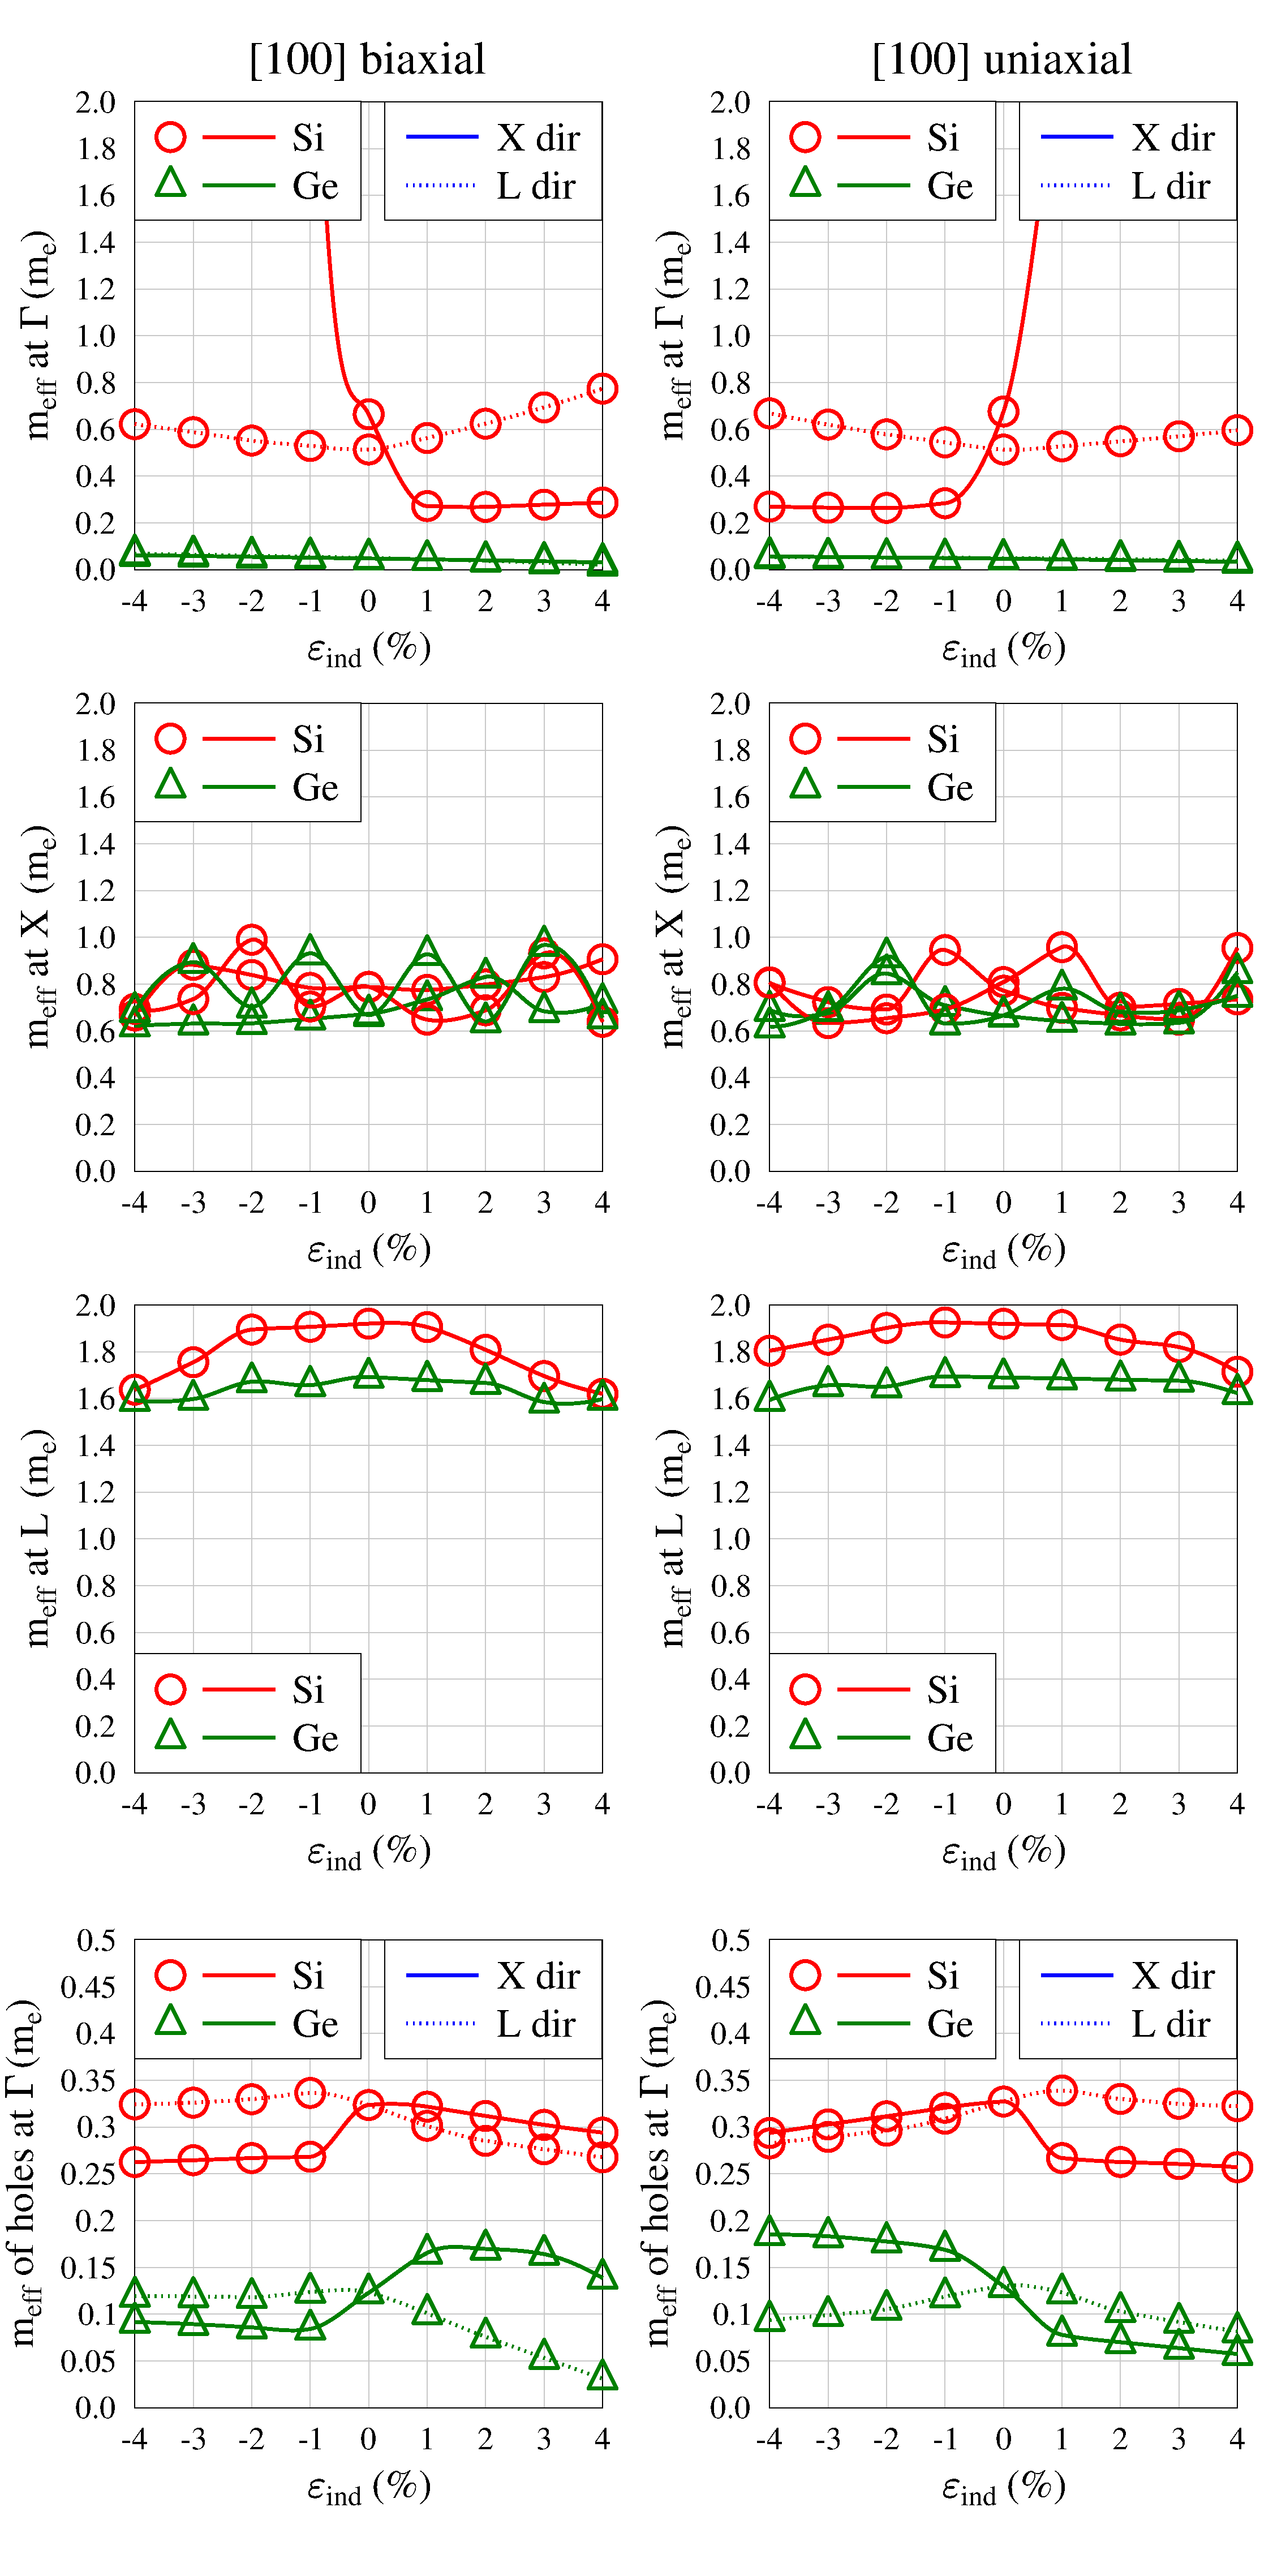
\includegraphics[width=0.7\textwidth]{strain/mass_100.pdf}
    \caption{Effective masses dependent on strains with respect to ${[100]}$ axis; red circles - Si, green triangles - Ge; at $\Gamma$: solid line - $\Gamma$-$X$ direction, dotted line - $\Gamma$-$X$ direction.} 
    \label{Fig:strain_mass_100}
\end{figure}

\begin{figure}[!htbp]
    \centering
    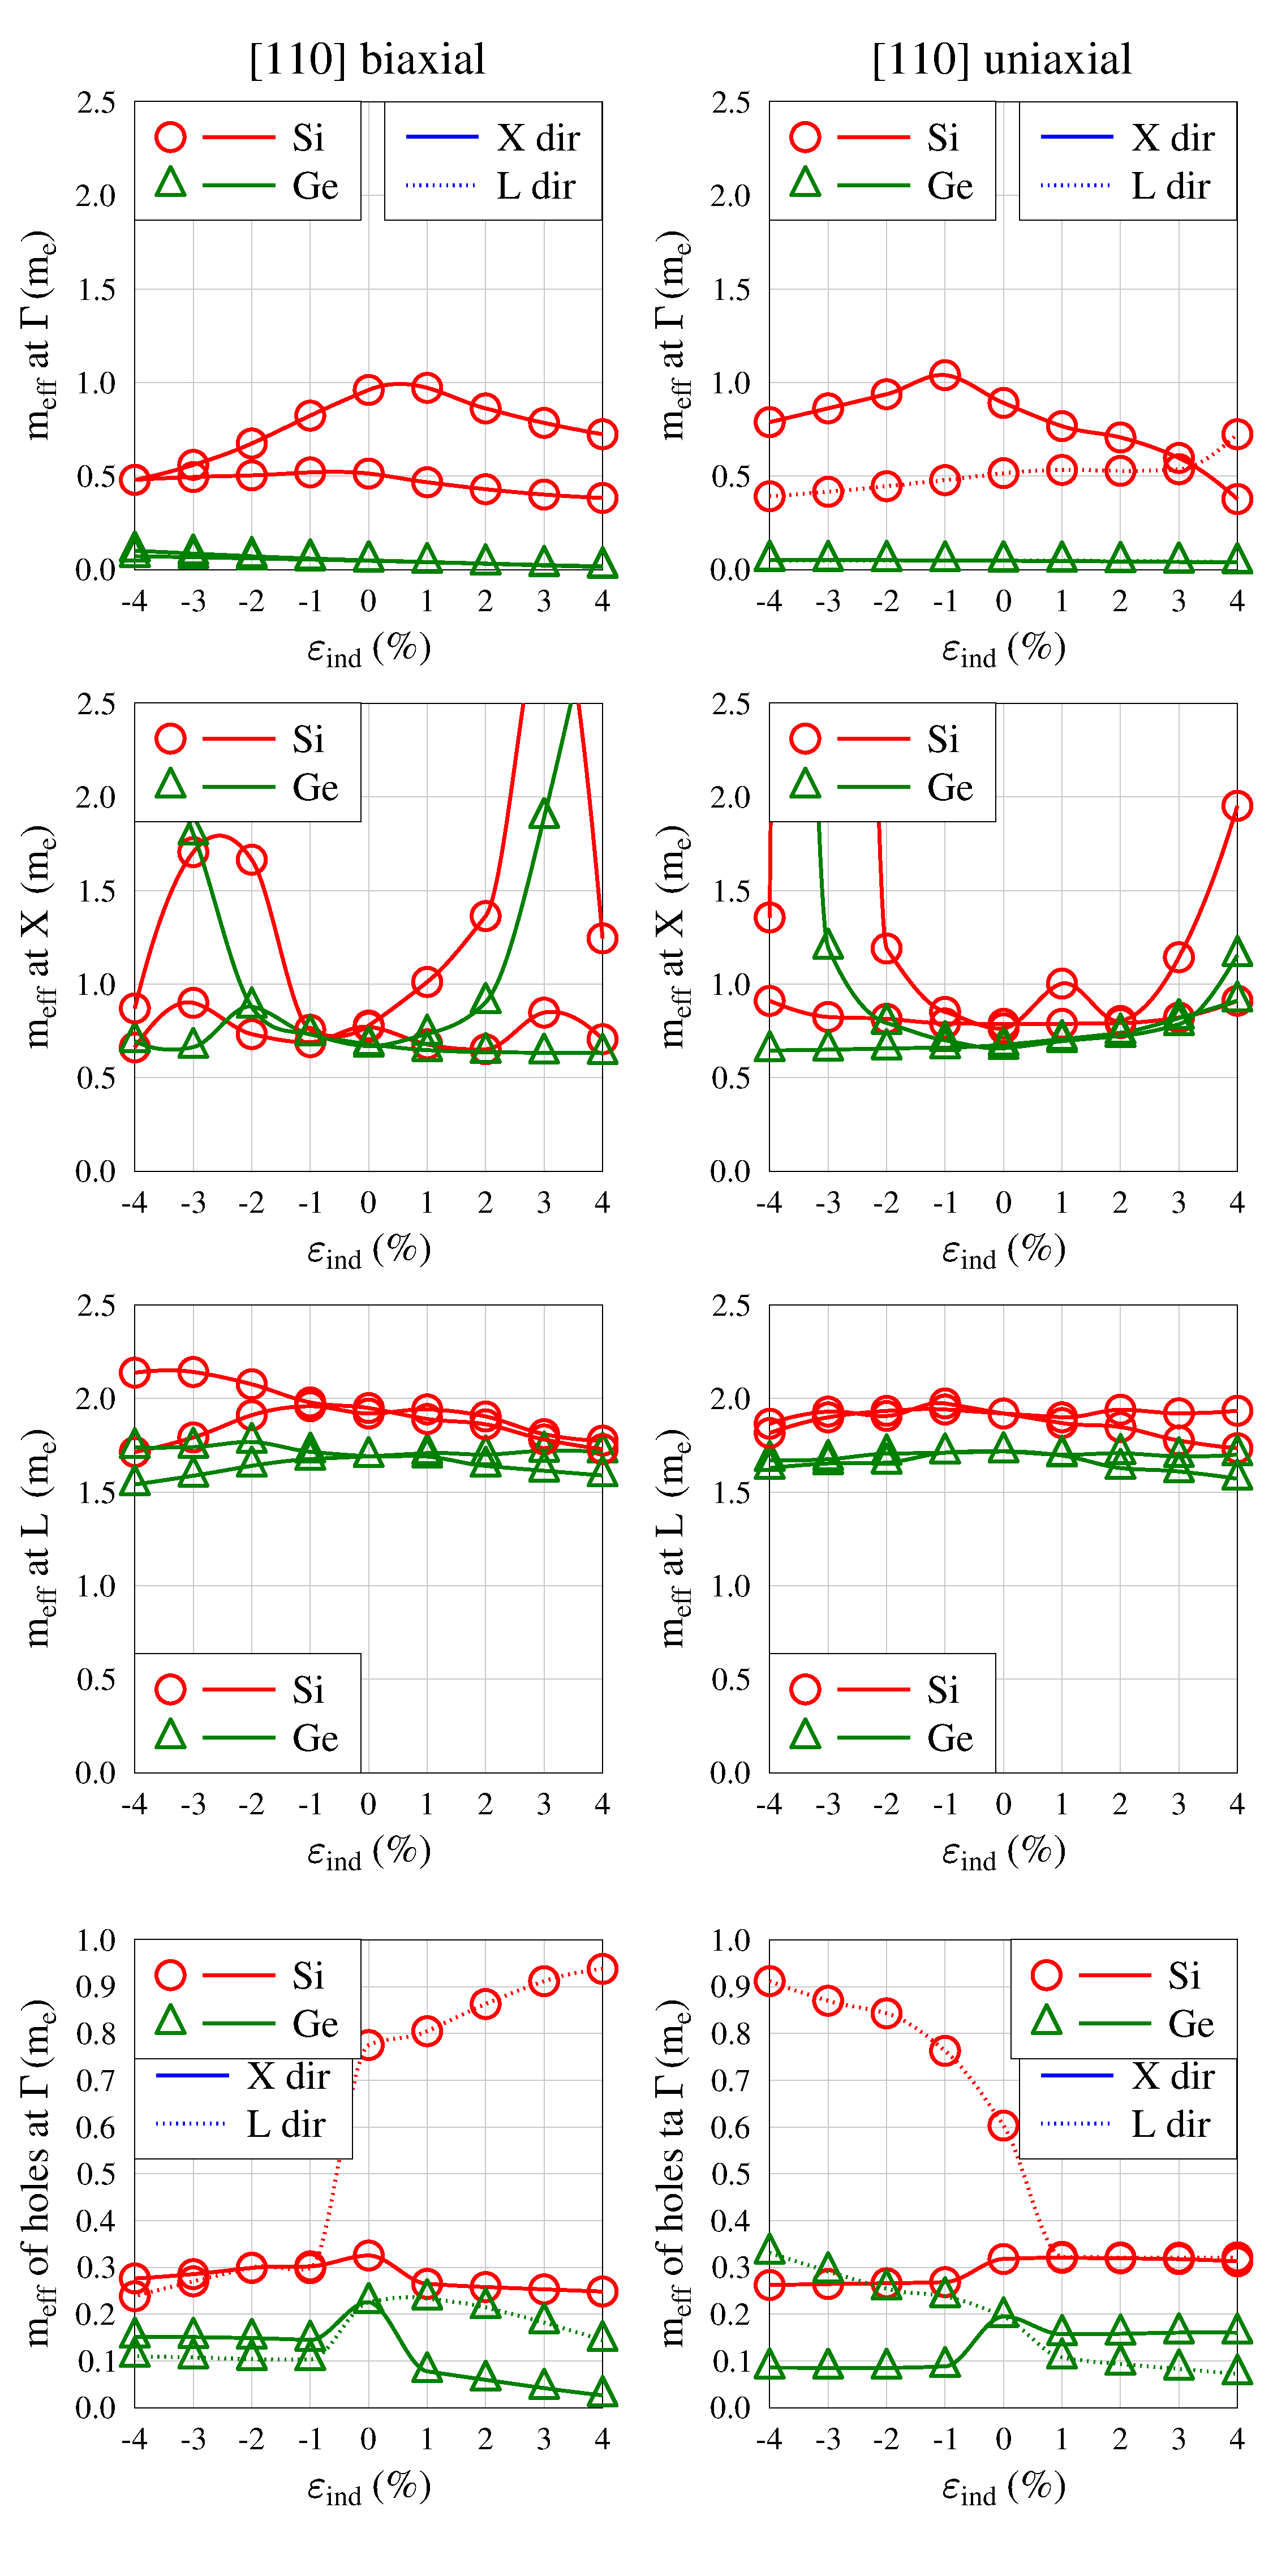
\includegraphics[width=0.7\textwidth]{strain/mass_110.pdf}
    \caption{Effective masses dependent on strains with respect to ${[110]}$ axis; red circles - Si, green triangles - Ge; at $\Gamma$: solid line - $\Gamma$-$X$ direction, dotted line - $\Gamma$-$X$ direction.} 
    \label{Fig:strain_mass_110}
\end{figure}

\begin{figure}[!htbp]
    \centering
    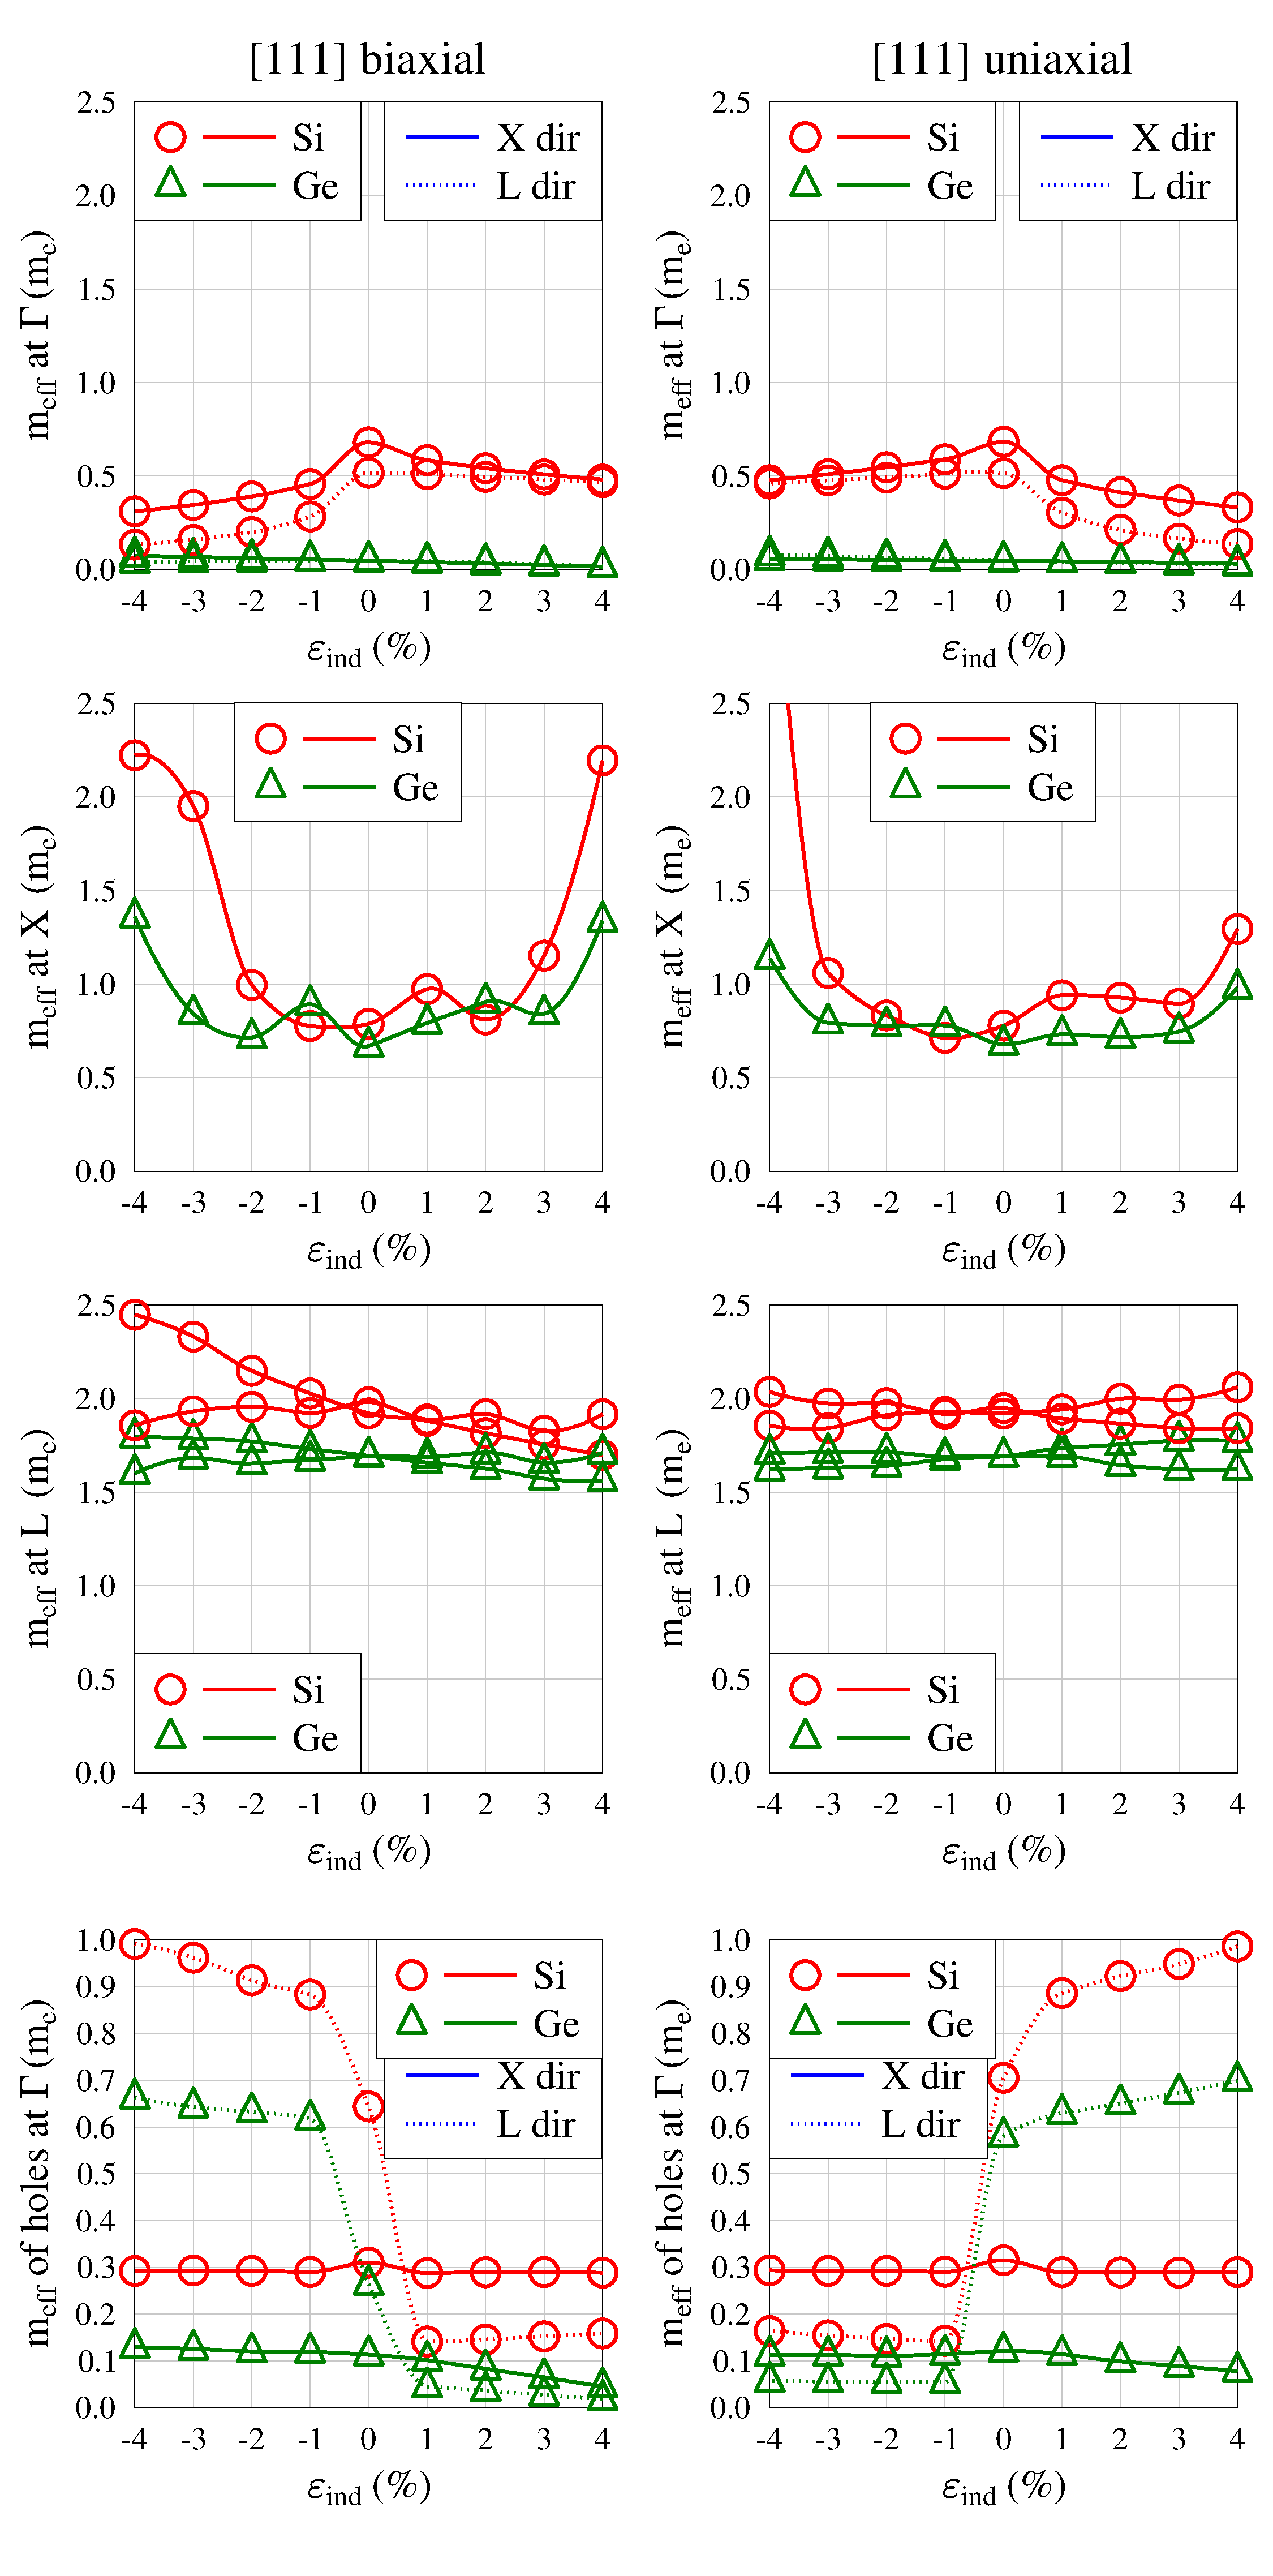
\includegraphics[width=0.7\textwidth]{strain/mass_111.pdf}
    \caption{Effective masses dependent on strains with respect to ${[111]}$ axis; red circles - Si, green triangles - Ge; at $\Gamma$: solid line - $\Gamma$-$X$ direction, dotted line - $\Gamma$-$X$ direction.} 
    \label{Fig:strain_mass_111}
\end{figure}

\begin{figure}[!htbp]
    \centering
    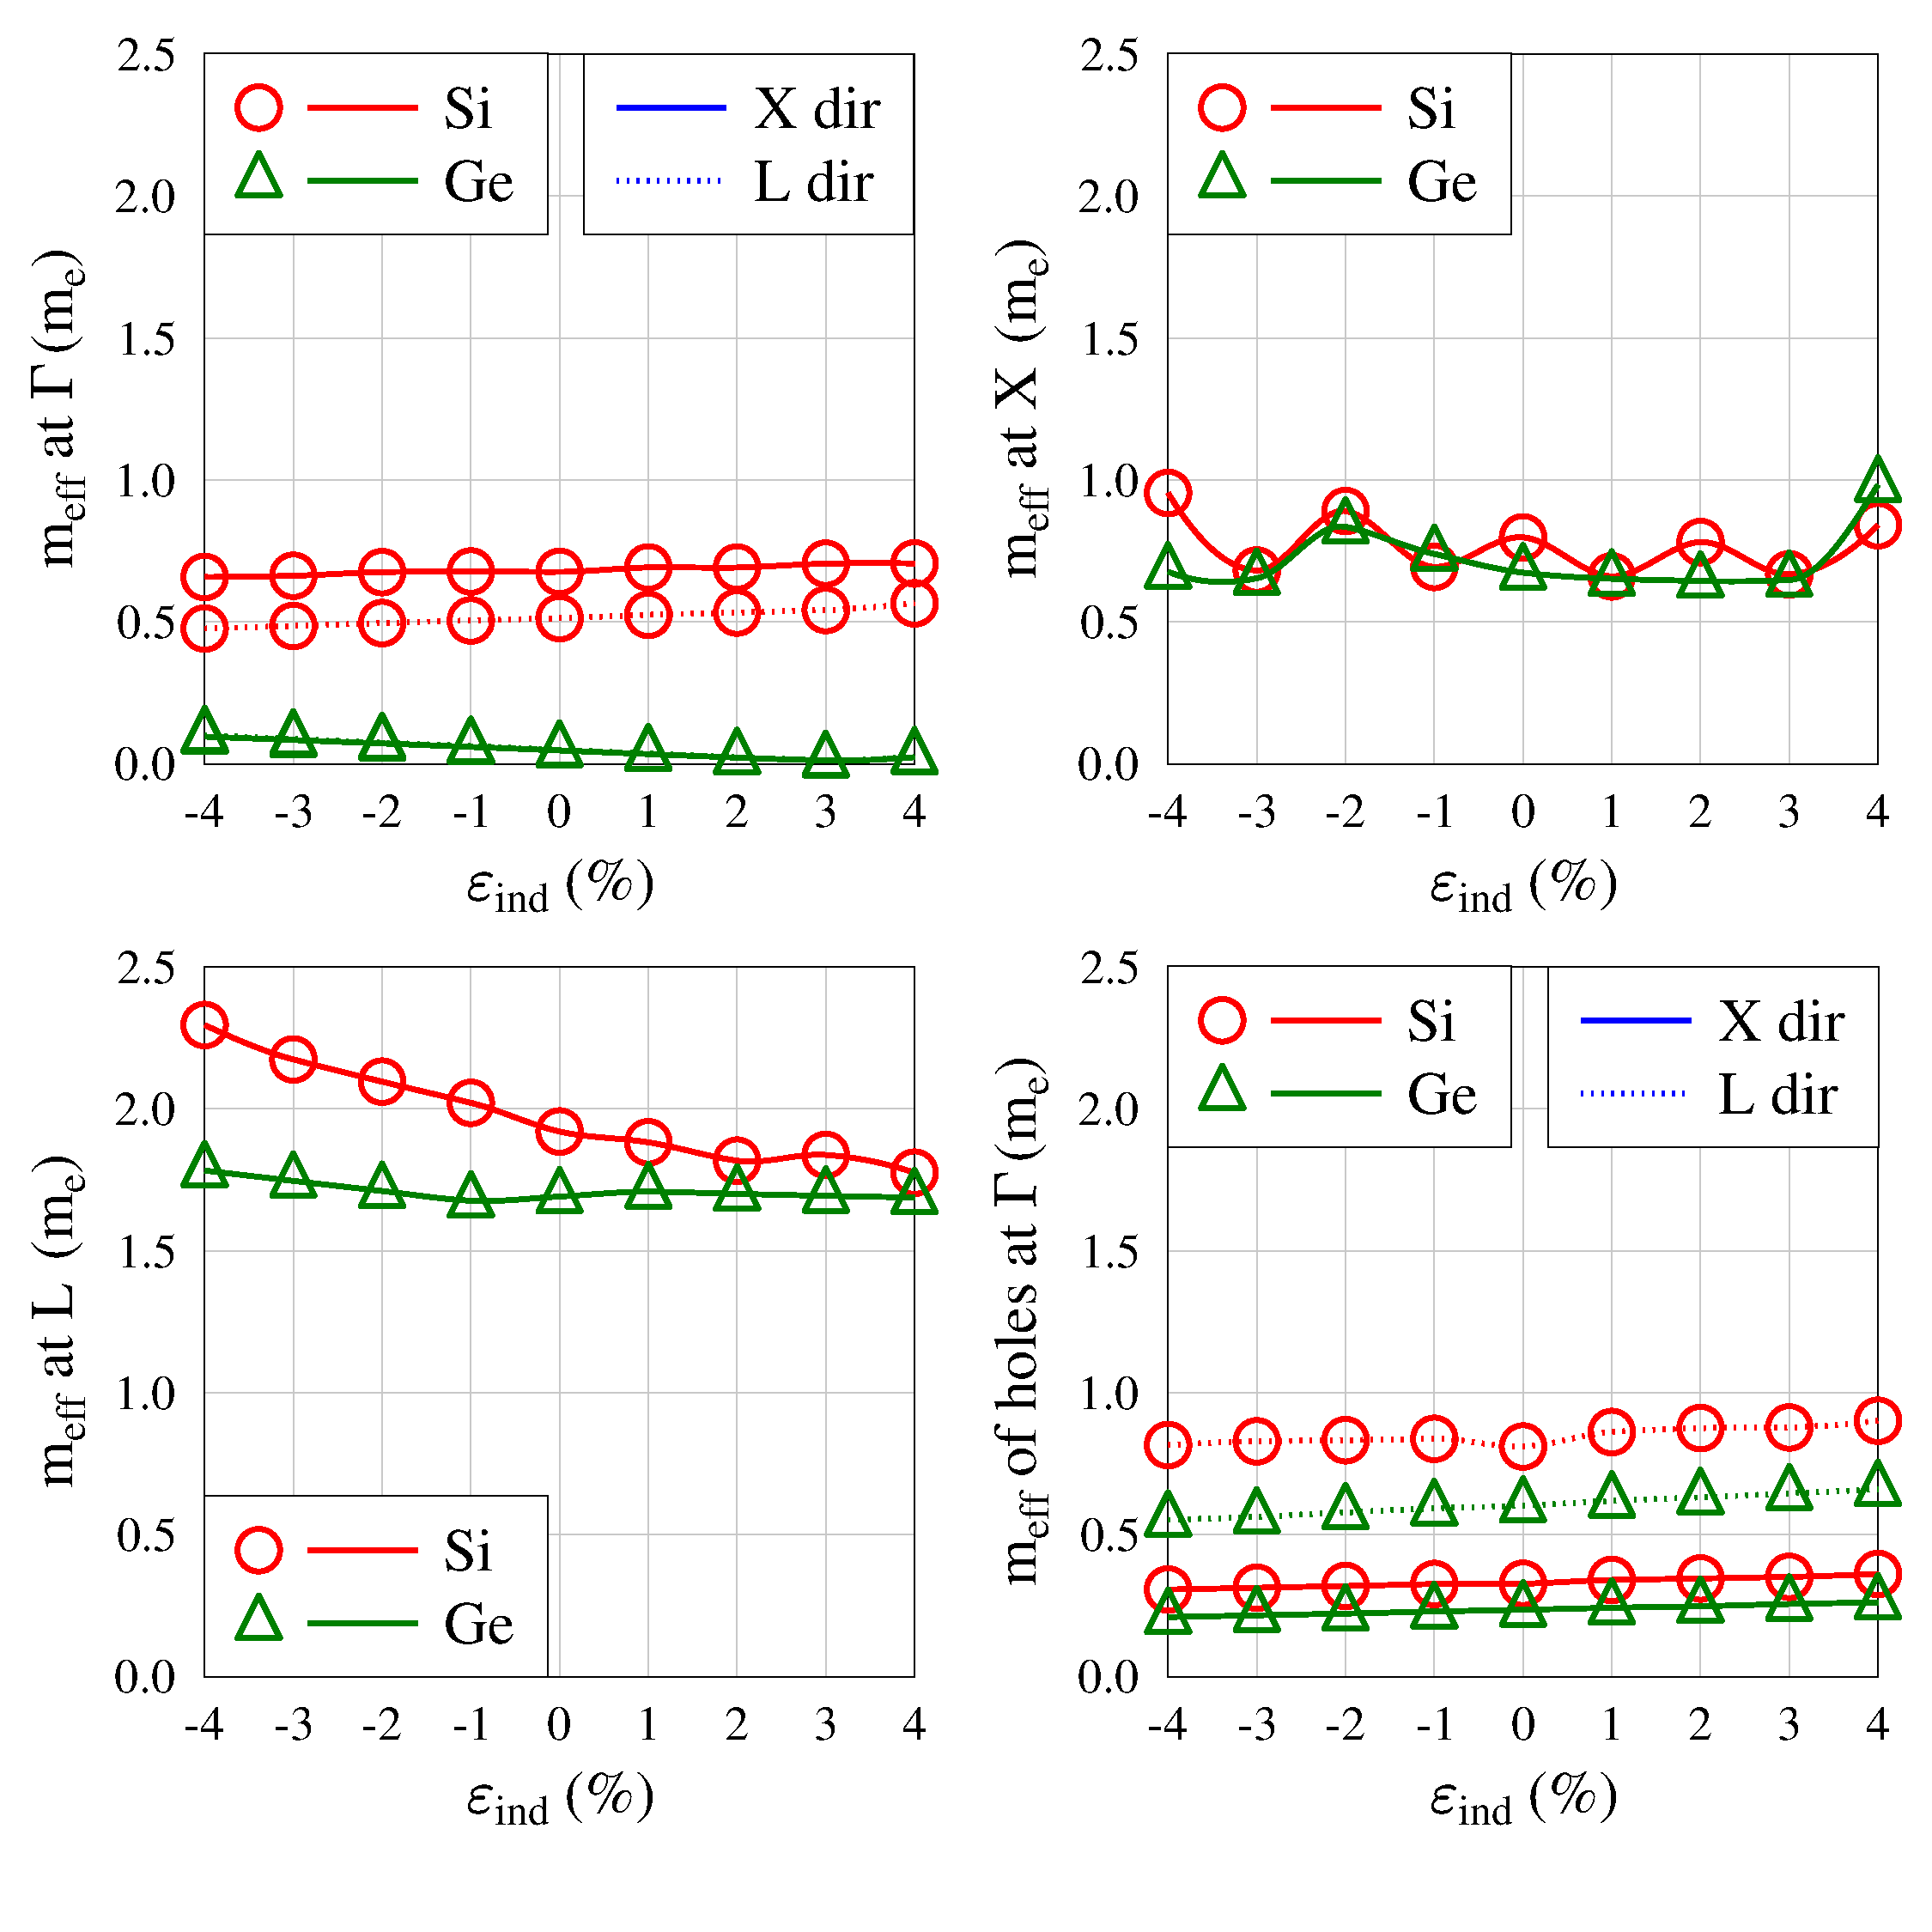
\includegraphics[width=0.7\textwidth]{strain/mass_iso.pdf}
    \caption{Effective masses dependent on isotropic strains; red circles - Si, green triangles - Ge; at $\Gamma$: solid line - $\Gamma$-$X$ direction, dotted line - $\Gamma$-$X$ direction.} 
    \label{Fig:strain_mass_iso}
\end{figure}
\newpage
\ornament

\section{Charge carriers mobility}

In addition to calculation of effective masses, the effect of strain on carrier mobility has been estimated.
The mobility is related to effective mass by scattering time, as follows
\begin{equation}
    \label{Eq:strain_mobility}
    \mu=\frac{q}{m^*}\bar{\tau},
\end{equation}
where $q$ is an elementary charge, and $\bar{\tau}$ is the average scattering time.
The scattering time, in general, depends on many factors connected with the scattering mechanisms which is not considered here.
Instead, an empirical model based on Monte Carlo simulations was used to evaluate the average scattering time for electrons \cite{scattering-time}:

\begin{equation}
\begin{split}
    \bar{\tau}_n =& \tau_0 + \tau_1 \cdot exp\Bigg(C_1 \cdot \bigg(\frac{T_n}{300 K}+C_0\bigg)^2 + \\
   & + C_2 \cdot \bigg(\frac{T_n}{300 K}+C_0\bigg) + C_3 \cdot \bigg(\frac{T_L}{300 K}\bigg) \Bigg) \\
\end{split}
\label{Eq:strain_time}
\end{equation}

where $T_n$ is the electron temperature, $T_L$ is the lattice temperature, while all of the $\tau$ and $C$ are material dependent constants (shown in Tab. \ref{Tab:strain_time}).
Formula \ref{Eq:strain_time} has been used here for calculating scattering time of electrons.
In the case of holes the scattering time is independent of carrier and lattice temperatures:
\begin{equation}
\label{Eq:strain_holes_time}
\bar{\tau}_p =\tau_2.
\end{equation}

\begin{table}[!htbp]
\centering
\caption{Material parameters for average scattering time  ( Eq. \ref{Eq:strain_time}) \cite{scattering-time}. $\tau$ are given in (ps).}
\begin{tabular}{|c|c|c|c|c|c|c|c|}
\hline
 & $\tau_0$ & $\tau_1$ & $C_0$ & $C_1$  & $C_2$ & $C_3$ & $\tau_2$ \\ \hline
Si       & 1             & -0.538        & 0     & 0.0015 & -0.09 & 0.17  & 0.4           \\ \hline
Ge       & 0.26          & 1.49          & 0     & -0.434 & 1.322 & 0     & 0.4           \\ \hline
\end{tabular}
\label{Tab:strain_time}
\end{table}

For given temperatures, the mobility changes are completely established by effective mass (Eq. \ref{Eq:strain_time}).
For unstrained materials the mobilities for both electrons and holes are known.
For Si it is $\leq 1400 \frac{cm^2}{V\cdot s}$ and $\leq 450 \frac{cm^2}{V\cdot s}$ for electrons and holes respectively, and for Ge similarly $\leq 3900 \frac{cm^2}{V\cdot s}$ and $\leq 1900 \frac{cm^2}{V\cdot s}$ (according to NSM Archive \cite{nsm}).
If we assume that the strain does not affect the scattering time, the strain dependent mobilities can be evaluated.
Examples of such calculations are presented in Fig. \ref{Fig:strain_mobility}.
First of all one can see that presented results agree well with tabular data at equilibrium state.
It can be also observed that the strain induced changes in effective masses affect significantly the mobilities.
In extreme cases they can change even by an order of magnitude.
 
 \begin{figure}[!htbp]
    \centering
    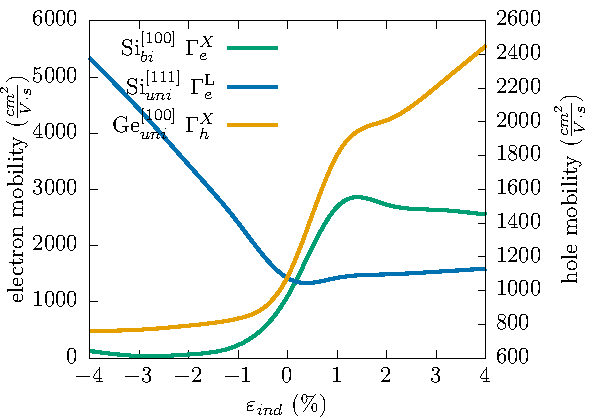
\includegraphics[width=0.7\textwidth]{strain/mobility.pdf}
    \caption{Carrier mobility examples calculated for $T_n,\,T_L=300 K$.} 
    \label{Fig:strain_mobility}
\end{figure}

\ornament

\section{Precision and accuracy of the results}

When \DFT\ results are presented the question about their precision and accuracy always arises.
The term ''precision'' in this context refers to the accuracy of calculations at given methods used within \DFT, i.e. their deviation from the exact result if it existed.
Since the ''exact'' result does not exist, the only way of estimating the precision is to compare the results with analogous ones, given by other codes, among which the full potential implementations seem to be most credible.
This issue is widely discussed in \cite{accuracy} where a special parameter $\Delta$ is introduced as a measure of discrepancy between \EOS\ for a sample of crystals calculated by a given pair of codes.
This parameter, when used in reference to full potential codes becomes a measure of precision.
In turn, the term ''accuracy'' refers to the agreement of computational results with experimental data, and it seems that an ultimate criterion to value various \DFT\ methods/codes is to compare the results with the experiment.
In the light of these remarks the discuss of the results presented is conducted below. 

The table in Fig.4 in \cite{offsets-Kresse} shows a comparisons of $\Delta$ parameter for most known \DFT\ methods, in reference to full-potential methods.
The PAW JTH/ABINIT, used in this work (in even newer version than in \cite{offsets-Kresse}), has there a very good ($0.6$) value.
Only VASP and various full potential codes show slightly better values (the lowest average value is $0.5$ and the highest is $13.3$).
In results presented here, this kind of \PAW\ datasets has been used in all the structural calculations and in the case of deformation potentials as well.
Taking into account that the rigorous convergence tests have been performed, the precision of presented results should be high.
Regarding the accuracy, it is also very satisfactory, as shows the comparison with the available experimental data.
E.g. the Tab. \ref{Tab:strain_lattice} shows an excellent agreement of the calculated lattice constants with experimental ones.
Also the elastic constants, although defined here in an unconventional way, when transformed to the standard ones agree well with the textbook data (see Tab. \ref{Tab:strain_elastic}).

\begin{figure}
    \centering
    \includegraphics[width=0.7\textwidth]{/strain/vs.pdf}
    \caption{Comparison between Wien2k (red line) and ABINIT with \mBJLDA\ (blue line) band structure of Ge in equilibrium state.} 
    \label{Fig:strain_wien-abinit}
\end{figure}

The calculations of band energies, gaps and effective masses have been performed using different method (\HGH\ joined with the \mBJLDA\ XC potential, see Sect. \ref{chap:methods}), and thus require a separate discussion of precision and accuracy.
As described in Sect. \ref{chap:methods}, the \mBJLDA\ cTB$09$ parameter (called here \textit{c}) has been fitted to get correct (experimental band gaps) and specially treated for strained systems (Eq. \ref{Eq:ctbo9}).
Figure \ref{Fig:strain_wien-abinit} shows a comparison of Ge band structure obtained in this work and by Wien2k code.
And one can see that the agreement is very good.
This means that conducted calculations are expected to be highly precise.
As far as the accuracy is concerned the agreement with the available experimental data shown in Fig. \ref{Fig:strain_exp} is very good. 

The accuracy of effective masses is an important issue to comment, since this is a known fact that the \mBJLDA\ functional overestimates effective masses by $20-30\%$ \cite{mbjlda_precision}, which is then a systematic error.
Surprisingly, the approach used in this work does not quite reflect this tendency.
As Tab. \ref{Tab:strain_masses} shows, the effective masses calculated here (in a very strict mathematical approach) sometimes are even lower than the experimental ones, but the overall agreement is quite satisfactory.
Nevertheless, the results presented here can certainly be regarded as a good qualitative picture (with rather low quantitative uncertainty) of masses vs. strains variation.

The calculations of the deformation potentials, particularly those describing the absolute changes in energies, are a delicate issue.
For the top of \VB, they have been done with the use of \PAW\ atomic datasets.
The same which gave very satisfactory structural parameters.
Here, the \DFT\ band gap problem does not exist since we consider only the \VB\ top energy with respect to the unified energy reference point.
Thus, the discrepancy of provided results with the literature data is surprising.
For this reason there have been included a precise description of the method used (see Chap. \ref{chap:methods}), so that the reproduction of the data or questioning the approach would be possible.

\ornament
		\chapter{Alloying}
\label{chap:alloying}

\section*{Chapter description}

In this chapter numerical results from alloys calculations are presented along with the analysis.
Beginning from elastic characteristics of investigated materials, e.g. lattice constants, lattice bowing, mixing parameter effect, moving to electronic properties.
Band structures and effective masses were calculated and described with details.
The discussion and most important conclusions are also underlined.
All calculations provided here were performed at the Wrocław Centre of Networking and Supercomputing.
In all the \abinitio\ calculations performed within this chapter, the ABINIT package \cite{abinit1} has been used, with \LDA, \HGH\ pseudopotentials \cite{abinit2, hgh}, Perdew and Wang correlation part of the functional \cite{pw} (\PAW), and the Tran and Blaha modified Becke Johnson functional TB-mBJ (sometimes referred to as \mBJLDA) \cite{tbtb} for the exchange part, known for quantitatively improving the electronic band structure while preserving a reasonable time of calculations.
As a result of convergence studies, the energy cutoff was set to $60$ Hartree, the k-points sampling for \BZ\ integration was ($10\times 10\times 10$) for all the calculations.
The energy convergence criteria in the \SC\ run was set to $10^{-9}$ Ha and the residual wave function convergence criteria in the non-\SC\ part was $10^{-12}$.
\ornament

\section{Mixing parameter}

In the beginning, the impact of the mixing parameter $\alpha$ on the band structure was tested.


The test performed have shown that the calculated \SC\ band structures rather weakly depend on the parameter $\alpha$, namely, when it is varied in the range $[0,1]$, the maximum band gap variation does not exceed $0.05$ eV.
Moreover, this effect is overshadowed by the adjusting procedure described in the next section.
In our calculations the value $\alpha=0.1$ has been used.

\ornament

\section{Lattice constant and c\_TB09}

The first step in \abinitio\ calculations is to obtain equilibrium lattice constants for chosen system corresponding to exchange--correlation functional and pseudopotential used.
That point was already covered in strain calculations \ref{chap:strains} and there is no need to repeat them.
The constants were taken from there \ref{Tab:strain_lattice} and applied to next steps.

From previous calculations also boundary condition (pure Ge and Sn) $c$ parameter was taken.

\ornament

\section{Mixing parameter}

At the beginning, the effect  of the mixing parameter $\alpha$ (Eq. \Ref{Eq:mixing}) on band structure was tested.

The tests performed have shown that the calculated band structures rather weakly depend on the parameter $\alpha$, namely, when it is varied in the range $[0,1]$, the maximum band gap variation does not exceed $0.05$ eV.
Moreover, this effect is overshadowed by the adjusting procedure described in the next section.
In provided calculations the value $\alpha=0.1$ has been used, to assure the symmetry breaking from diamond to \BZ, induced by the fact that the alchemical atoms in the \prim\ are not the same. One should note that in the alloy there is no symmetry at all, except for identity, but the \BZ\ symmetry emerging in \AM\ approach has no effect on the results but speeds up the calculations.   

\ornament

\section{AM vs. supercell band structure}

As described in the previous section the aim of this work was to reproduce the unfolded supercell band structure with the smooth curves given by \DFT\ \AM\ approximation, in particular a proper behavior of the direct and the indirect band gaps.
Two parameters: the lattice constant $a$ and the $c$ (c\_TB09) have been found, for the parent materials Ge and Sn, and for the alloy at composition $x$ via the bowing parameter $b$ in Vegard's law \Ref{eq:Vegard_quad}.
For practical reasons only the range up to $\approx 30\%$ (closing the band gap) has been considered in this work.
As a reference the data from \cite{Polak_2017} have been used.
The results are given in Tab. \ref{Tab:alloy_params}. 

\begin{table}[]
	\begin{center}
		\caption{Lattice and $c$ parameters achieved from fitting procedure.}
		\label{Tab:alloy_params}
		\begin{tabular}{|c|c|c|c|}
			\hline
			parameter                           & Ge     & Sn    & $b$ \\ \hline
			lattice const. (\AA) & 10.636 & 12.25 & -1.08    \\ \hline
			c\_TB09                             & 1.037  & 0.99  & -0.02    \\ \hline
		\end{tabular}
	\end{center}
\end{table}

In Fig. \ref{Fig:alloy_band_gaps} the \AM\ and the \DFT\ supercell band gaps (\cite{Polak_2017}) variations, direct and indirect, are compared, and it can be seen that in the range of composition of interest the agreement is very satisfactory, the discrepancy is not higher than $0.03$ eV. 

To validate the method even more, in Fig. \ref{Fig:AMvsSC} the band structures for parent materials, Ge and Sn, and the unfolded GeSn alloy band structures for chosen compositions (from \cite{Polak_2017}) are compared with those obtained in this work.
It can be seen that the smooth \AM\ curves provide a very good approximation for the supercell bands.  


\begin{figure}[!htbp]
	\centering
	\includegraphics[width=1\textwidth]{/alloys/GeSn-gap.pdf}
	\caption{Band gaps from AM calculations vs supercell ones taken from \cite{Polak_2017}; red -- direct, blue -- indirect.}
	\label{Fig:alloy_band_gaps}
\end{figure}



\begin{figure}[!htbp]
	\centering
	\subfloat[Pure Ge.]{\includegraphics[width=.45\textwidth]{/alloys/Ge_EIG.pdf}}\quad
	\subfloat[$\textrm{Ge}_{0.963}\textrm{Sn}_{0.037}$.]{\includegraphics[width=.45\textwidth]{/alloys/GeSno_3_7.pdf}}\\
	\subfloat[$\textrm{Ge}_{0.87}\textrm{Sn}_{0.13}$.]{\includegraphics[width=.45\textwidth]{/alloys/GeSno_13.pdf}}\quad
	\subfloat[Pure Sn.]{\includegraphics[width=.45\textwidth]{/alloys/Sn_EIG.pdf}}
	\caption{AM vs supercell band structures -- continuous blue line represents AM results.}
	\label{Fig:AMvsSC}
\end{figure}

Finally, the effective masses of electrons at $\Gamma$ and $L$ valleys have been evaluated and compared with those reported in \cite{Polak_2017}. Also in this case the agreement is very good which confirms the validity of the method. 

\begin{figure}[!htbp]
	\centering
	\includegraphics[width=.7\textwidth]{/alloys/GeSn-mass.pdf}
	\caption{Effective masses of electrons in open gap $\textrm{Ge}_x\textrm{Sn}_{1-x}$; red/green -- $\Gamma$ valley, blue -- $L$ valley.}
	\label{Fig:alloy_mass}
\end{figure}

To summarize, in this work the computational alchemy approximation has been used to represent the \DFT\ supercell electronic band structure of GeSn alloy with smooth, well fitted curves.
The results have been used in \cite{janik.2021} to represent the band structure with the 30--bands $\mathbf{k}\cdot\mathbf{p}$ method, suitable in semiconductor device modelling.

\ornament
		\chapter{Structural Factor}
\label{chap:wurtzite}

\section*{Chapter description}

This chapter presents the structural, elastic and electronic properties of group IV materials (C, Si and Ge) in the wurtzite structure, with particular emphasis on the effects of strain. The first part focuses on the equilibrium structural parameters, including lattice constants and the internal parameter \(u\), as well as the bulk moduli, elastic constants, pressure coefficients and Poisson's ratios. The stability of the wurtzite phase is also examined by comparing its formation energy with that of the zinc blende structure under different strain conditions.


The second part is devoted to the electronic properties of the investigated materials. Their band structures, fundamental band gaps, spin-orbit and crystal-field splittings, and deformation potentials are analysed. Particular attention is paid to strain-induced changes in the character and magnitude of the fundamental band gap, as well as to the effective masses of electrons and holes. The results reveal the possibility of inducing a direct band gap in selected materials and highlight the potential of wurtzite Ge for infrared optoelectronic applications. Finally, the calculated results for Si are compared with available theoretical reference data, providing a basis for assessing the reliability of the present calculations.


All calculations provided here were performed at the Wrocław Centre of Networking and Supercomputing.
In all the \abinitio\ calculations performed within this chapter, the VASP package \cite{vasp1} has been used, with \LDA, \PAW\ pseudopotentials \cite{vasp2, paw}, Perdew and Wang correlation part of the functional \cite{pw} (\PAW), and the Tran and Blaha modified Becke Johnson functional TB-mBJ (sometimes referred to as \mBJLDA) \cite{tbtb} for the exchange part.
\ornament

\section{Structural and elastic properties}

As in the Chapt. \ref{chap:strains}, the investigations began with achieving parameters of equilibrium wurtzite structures for investigated materials (C, Si and Ge).
The symmetry of this type of systems has a unique feature.
Some of the atomic sites may flow along $c$ lattice vector direction without changing the symmetry.
Thus an additional parameter $u$ is present in the relaxation procedure.
In Fig. \ref{Fig:wz_cell} blue arrow represents $\Vec{c}$ lattice vector, while orange one represents $u\cdot \Vec{c}$.
The bulk modulus $B_0$, it's pressure derivative $B'_0$ and elastic constants (from $c_{11}$ to $c_{33}$) were also evaluated.
\begin{table}[!htbp]
	\centering
	\caption{Elastic parameters.}
	\label{Tab:wz_elastic}
	\begin{tabular}{|c|c|c|c|c|}
		\hline
		& C & Si & Si--ref \cite{wz_si_strain_dft} & Ge \\ \hline
		a (\AA) & 2.498 & 3.823 & 3.828 & 4.005 \\ \hline
		c (\AA) & 4.159 & 6.323 & 6.325 & 6.594 \\ \hline
		u & 0.374 & 0.374 & 0.374 & 0.375 \\ \hline
		$B_0$ (GPa) & 450 & 94 & 92.8 & 67 \\ \hline
		$B'_0$ & 3.65 & 4.57 & 4.24 & 4.71 \\ \hline
		$c_{11}$ (GPa) & 1219 & 187 & 237 - $c_{12}$ & 125 \\ \hline
		$c_{12}$ (GPa) & 106 & 54 & 237 - $c_{11}$ & 54 \\ \hline
		$c_{13}$ (GPa) & 19 & 38 & 317 & 22 \\ \hline
		$c_{33}$ (GPa) & 1332 & 213 & 313 & 162 \\ \hline
	\end{tabular}
\end{table}

The only reference data found in the literature are for Si \cite{wz_si_strain_dft}.
Very satisfactory agreement of these data with those obtained in this work can be seen (see Tab. \Ref{Tab:wz_elastic}). The lattice constants differ on third decimal point, while the bulk modulus and the elastic constants differ no more than 10 GPa.

In Tab. \ref{Tab:wz_pressure} the pressure related to isotropic strain is presented in the form of the linear ($b$) and the quadratic ($a$) coefficients.  

\begin{table}[!htbp]
	\centering
	\caption{Pressure coefficients.}
	\label{Tab:wz_pressure}
	\begin{tabular}{|c|c|c|c|}
		\hline
		& C & Si & Ge \\ \hline
		$a$ (GPa) & -0.79 & -0.19 & -0.14 \\ \hline
		$b$ (GPa) & 13.45 & 2.81 & 2.00 \\ \hline
	\end{tabular}
\end{table}

The Poisson ratios, both for uniaxial and biaxial strains are shown in  Tab. \ref{Tab:wz_Poisson}.

\begin{table}[!htbp]
	\caption{Poisson's ratios ($\nu$) for axial (type 1) and biaxial (type 2) strains.}
	\centering
	\begin{tabular}{|c|c|c|}
		\hline
		material & 1 & 2 \\ \hline
		C     & 0.02        & 0.03  \\ \hline
		Si    & 0.16        & 0.38  \\ \hline
		Ge    & 0.13        & 0.29  \\ \hline
		Sn    & 0.18        & 0.44  \\ \hline
	\end{tabular}
	\label{Tab:wz_Poisson}
\end{table}

The formation energies as functions of strain are presented in Fig. \ref{Fig:wz_formation}

\begin{figure}[!htbp]
	\centering
	\includegraphics[width=.8\textwidth]{/wurtzite/formation.pdf}
	\caption{Formation energy of group IV materials (calculated as energy per atom in zinc blend minus wurtzite). $pl$ stands for planar strains in zinc blend (111) and wurtzite (001), while $iso$ stands for isotropic strains for both systems.}
	\label{Fig:wz_formation}
\end{figure}

Because of the lack of experimental data, the elastic properties are compared with those of the zinc blend ones.
Despite the change in the structure, the chemical trends are preserved.
Both the elastic constants and the bulk modulus are very high for C and decrease while moving downward the periodic table.
The related to isotropic strains hydrostatic pressure also shows the toughness of diamond.
As in zinc blend structure, wurtzite systems show slight non--linear behaviour of pressure induced by strain.
Calculated Poisson's ratios shows similar behavior to the zinc blende ones.
At biaxial strains they are bigger than at axial ones, and the more massive atom the higher is the value (with exception of Ge, which has  lower value than for Si). On the contrary, the ratios do not exceed 0.5, even in biaxial cases.

The analysis of the formation energy as dependent on strain shows that only Sn seems to energetically prefer the wurtzite structure,  under tensile isotropic strain.
In every other case, preferable is the zinc blend structure.
Moreover, the more strained system (no matter compressive or tensile) the more energetically preferable is the zinc blend over wurtzite structure.
On the other hand, the value of difference of energy per atom is rather small (excluding isotropic Sn, below $-0.001\ eV$) which means that the  energetic criterion is of a lower meaning in determination of system preferences.

\ornament

\section{Electronic structure}

The second part of the results concern the electronic structure properties.
As in Chpt. \ref{chap:strains}, the main focus is given to strain effects. In the first step the electronic band structures along  paths containing high symmetry directions have been evaluated. 
This allowed us to the find direct and the indirect gaps and, what is of crucial meaning, to identify the fundamental gaps. In the following steps the effective masses at band extrema have been evaluated and finally the deformation potentials. Table \ref{Tab:wz_electronic} shows the basic parameters at equilibrium state along with deformation potentials for each of the investigated materials.

\begin{table}[!htbp]
	\centering
	\caption{Electronic band structure parameters.}
	\label{Tab:wz_electronic}
	\begin{tabular}{|c|c|c|c|}
		\hline
		& C & Si & Ge \\ \hline
		$E_g^\Gamma$ (eV) & 6.517 & 1.649 & 0.362 \\ \hline
		$E_g^M$ (eV) & 5.800 & 1.015 & 0.897 \\ \hline
		$E_g^K$ (eV) & 5.318 & 1.471 & 1.879 \\ \hline
		$\Delta_{so}$ (eV) & 0.011 & 0.048 & 0.272 \\ \hline
		$\Delta_{cr}$ (eV) & 0.516 & 0.351 & 0.251 \\ \hline
		$D_1$ & 0.43 & 5.38 & 0.34 \\ \hline
		$D_2$ & 0.50 & 0.46 & -0.07 \\ \hline
		$D_3$ & 0.16 & 3.59 & 0.19 \\ \hline
		$D_4$ & 0.225 & 0.24 & 1.31 \\ \hline
		$D_5$ & 0.275 & 1.18 & 1.1 \\ \hline
		$D_6$ & 0.24 & 0.27 & 0.64 \\ \hline
	\end{tabular}
\end{table}

There is no reference data for the deformation potentials but they seem to have reasonable values.
The method itself for calculating the deformation potentials is precisely described and have strong physical foundations as well as the parameters used for \abinitio\ calculations were rigid.

The table above \ref{Tab:wz_electronic} shows in particular the gaps for Ge, which proves that there is a direct band gap at equilibrium state.
As for the other materials, the indirect band gap prevails but certain perspective still exists that under the strain the situation may change in favour of the direct band gap.
To observe this,  the fundamental band gaps under strain are presented (Fig. \ref{Fig:wz_fundamental} along with effective masses of carriers (Fig. \ref{Fig:wz_mass}) at $\Gamma$ k--point (for holes) and at fundamental gap k--point (for electrons). Both in $\Delta$ and $\Lambda$ directions.


\begin{figure}[!htbp]
	\centering
	\subfloat[][Fundamental band gaps.\label{Fig:wz_fundamental}]{\includegraphics[width=.45\textwidth]{/wurtzite/WZ-gap.pdf}}\quad
	\subfloat[][Effective mass of charge carriers.\label{Fig:wz_mass}]{\includegraphics[width=.45\textwidth]{/wurtzite/WZ-mass.pdf}}
	\caption{Band structure parameters in wurtzite system group IV materials.}
\end{figure}

In Fig. \ref{Fig:wz_fundamental} one can see that in the case of Ge the direct band gap appears at  almost all applied strains.
Only at biaxial compressive strain higher than 2\%, the gap is indirect. 
Moreover, the value of the direct gap may vary from actually closed one (at biaxial tensile and axial compressive strain) to even more than $0.6\ eV$ (in isotropic compressive strain).
This fact together with the fact that the effective masses of electrons and holes in $\Delta$ direction are below $0.2\ m_e$, opens interesting perspectives  for  applications of this material in infrared optoelectronics.
Apart from Ge, only Si appears to have direct band gap under biaxial tensile strain, but only above 4\%, which is a quite high value.

The data obtained in this work for Si can be compared with the literature data  \cite{wz_si_strain_dft}, which are also theoretical.
The lattice constants  differ on second decimal point and the fundamental band gap value differs around 0.2 eV, although the type of gap is the same ($\Gamma-M$).
The equilibrium state band gaps are almost the same. The transitions of type of fundamental gap is exactly at the same strain value for all three straining types.
The difference can be seen in the slope of band gap changes, in presented results it is slightly lower and in biaxial strains the parabolic behaviour is more distinct, unlike in the reference.
Nevertheless, the agreement is good enough to enhance the credibility of the rest of the investigated materials.

For the full picture $\Delta_{so}$ and $\Delta_{cr}$ were also calculated for all the types of strains and their range. 
The results are shown in the Fig. \ref{Fig:wz_delta}.
\begin{figure}[!htbp]
	\centering
	\includegraphics[width=.8\textwidth]{/wurtzite/WZ-delta.pdf}
	\caption{Strain dependence of $\Delta_{so}$ and $\Delta_{cr}$ in wurtzite group IV systems.}
	\label{Fig:wz_delta}
\end{figure}

While there are almost no changes in the $\Delta_{so}$ parameters, the $\Delta_{cr}$ vary significantly, up to 4-times in Ge at biaxial strain. 

\ornament
		\chapter{Spacial Confinement}
\label{chap:digital}

\section*{Chapter description}

This chapter presents a preliminary investigation of spatial confinement effects and the electronic structure of Ge–Si digital alloys. The study focuses on layered systems grown along the [100] direction, considering both Si and Ge substrates. After verifying the consistency of the structural parameters obtained from the relaxation and Poisson's ratio calculations, the electronic band structures are analysed along a Brillouin zone path that accounts for both in-plane and out-of-plane directions.

Particular attention is given to the atomic contributions to the electronic states, investigated through atom-projected band structures. The results reveal interesting features, including direct and indirect band gaps, band folding effects, and differences in the electronic structure depending on the substrate material. The analysis suggests that the Ge–Si digital alloy may exhibit spatially dependent electronic properties, potentially resembling those of a quantum well system, with distinct band-gap characteristics along the direction perpendicular to the layers.

The results demonstrate the potential of Ge–Si digital alloys as systems for further studies of spatial confinement and electronic properties in layered materials. They also identify several important questions for future research, including the influence of layer thickness, the effect of growth along the [111] direction, the spatial distribution of band gaps, and the optical properties associated with possible electronic transitions. The possibility of extending this approach to digital alloys with wurtzite structures is also discussed.

\ornament

\section{Atomic Positions}

In the beginning, Poisson's ratio test results were evaluated.
The difference of atomic positions and lattice vectors between relaxation procedure and Poisson's ratio on testing structures prove to be on the fourth decimal point or below.
This is sufficient enough to use Poisson's ratio and atomic position of previous calculations instead of relaxation procedure.
It should be stated here that this was possible only due to the usage of the same \XC\ functional and pseudopotential  as it was practiced in the investigations of the strain effects (Chpt. \ref{chap:strains}).

\ornament

\section{Band structure}

Although the bulk crystal structures of the component materials are the the diamond ones, due to layered nature, the \BZ\ of the system differs (as it has been explained above).
It is not known to which points the focus should be given so the path was chosen to cover all of the characteristic points and to be the most representative.
For the [100] direction the path was set to $Y-\Gamma-X-U-Z-\Gamma$.
The crucial criterium was to cover both in--plane and along crystal growth directions to analyze how the electrons will behave in both directions.

\begin{figure}[!htbp]
	\centering
	\subfloat[][Band structure.]{\includegraphics[width=.96\textwidth]{/digital/bandSi.pdf}}\\
	\subfloat[][$Ge_1$]{\includegraphics[width=.48\textwidth]{/digital/fatband1Si.pdf}}\quad
	\subfloat[][$Ge_2$]{\includegraphics[width=.48\textwidth]{/digital/fatband2Si.pdf}}\\
	\subfloat[][$Si_1$]{\includegraphics[width=.48\textwidth]{/digital/fatband3Si.pdf}}\quad
	\subfloat[][$Si_2$]{\includegraphics[width=.48\textwidth]{/digital/fatband4Si.pdf}}
	\caption{Atomic decomposition of band structure of [100] direction on Si substrate.}
	\label{Fig:da_fbnd_si_1_100}
\end{figure}

\begin{figure}[!htbp]
	\centering
	\subfloat[][Band structure.]{\includegraphics[width=.96\textwidth]{/digital/bandGe.pdf}}\\
	\subfloat[][$Ge_1$]{\includegraphics[width=.48\textwidth]{/digital/fatband1Ge.pdf}}\quad
	\subfloat[][$Ge_2$]{\includegraphics[width=.48\textwidth]{/digital/fatband2Ge.pdf}}\\
	\subfloat[][$Si_1$]{\includegraphics[width=.48\textwidth]{/digital/fatband3Ge.pdf}}\quad
	\subfloat[][$Si_2$]{\includegraphics[width=.48\textwidth]{/digital/fatband4Ge.pdf}}
	\caption{Atomic decomposition of band structure of [100] direction on Ge substrate.}
	\label{Fig:da_fbnd_ge_1_100}
\end{figure}

As a preliminary results, in Figs. \ref{Fig:da_fbnd_si_1_100} and \ref{Fig:da_fbnd_ge_1_100} the band structures are shown for the cases of (100) plane and Si and Ge substrates, together with the decomposition for each atom in elementary cell. Some interesting features of the band structures can be observed. In both systems the direct gap of the order of $1eV$ can be observed, which is presumably a result of  Si $\Gamma$-$X$ band folding. However, in the case of Si substrate, the fundamental gap seems to be indirect, from $\Gamma$ point to $U$ point, but the situation looks different when looking at the atom projected band structures. Here, considering the Ge2 and Si1 atoms, the band gap is direct. Moreover, the $X-U$ direction is perpendicular to the layered system, and a question arises about spatial distribution of band gap energies in the direction perpendicular to the layered systems. Here, a kind of quantum well system can be expected, which can be studied by evaluating the spatially resolved band gaps, for the vertical direction. In the case of Ge substrate the band gap is direct around $\Gamma$, is smaller than $1eV$, and in the direction $\Gamma-Z$ (perpendicular to the layers) has a nesting character, wheres at $U$ point the bands at CB minimum are degenerate. 

The presented results show that the idea of the Ge-Si digital alloy is promising and deserves further attention.  Some interesting features of electronic band structures have been demonstrated here, leading to important questions which should be addressed: 1. what is the effect of increasing number of a given material layers, 2. how the band structures will look like for (111) direction, 3. how the spatially resolved band gaps (in the  vertical direction) behave, and what are the consequences of this behavior for optical properties, 4. what are the oscillator strengths of identified possible optical transitions, and how they, together with the energetic structure affect the optical response. Another intriguing  perspective is an extension of the  investigations on the Ge-Si digital alloys in wurtzite structures, discussed in Chpt. \ref{chap:wurtzite}, where germanium exhibits already a direct fundamental gap, independently of strains, and the role silicon should be determined. Here, the c-direction seems to be natural to form such an alloy, and the band folding in this direction can introduce unpredicted effects. All those issues will be a subject of the planned further investigations.

\ornament
		%\input{02-Mainmatter/Chapter9.tex}
		
		```latex
\chapter*{Conclusion}
\addcontentsline{toc}{part}{Conclusion}

\section*{Summary and conclusion}

The main objective of this thesis was to investigate the possibilities of electronic structure engineering in group IV crystals, with particular emphasis on materials compatible with the existing silicon-based technology and potentially suitable for optoelectronic applications. Four approaches to modifying the electronic structure were considered: strain, alloying, structural modifications, and quantum confinement. The calculations were performed within the framework of density functional theory, using different computational approaches and exchange--correlation functionals depending on the properties under investigation.

The results demonstrate that even relatively simple modifications of group IV crystal structures can lead to substantial changes in their electronic properties. In particular, the fundamental band gap, its direct or indirect character, band offsets, and effective masses can be strongly affected. At the same time, the investigations provide structural and elastic parameters that are relevant for understanding and predicting the response of these materials to external or internally induced modifications.

\subsection*{Chapter~\ref{chap:strains} -- Strain engineering}

The aim of this part of the work was to provide a systematic description of the influence of technologically relevant strains on the electronic structures of group IV crystals in the diamond structure. Isotropic, uniaxial, and biaxial strains were investigated, with the latter two applied along the crystallographically relevant $[100]$, $[110]$, and $[111]$ directions.

The calculations have shown that strain produces significant changes in the band structures, particularly in the fundamental band gaps and the relative positions of the band extrema. Depending on the material, strain type, and crystallographic direction, transitions between direct and indirect band gaps can occur. The symmetry reduction associated with non-isotropic strains also leads to the splitting of formerly degenerate states at selected high-symmetry points of the Brillouin zone. These effects demonstrate that the electronic response cannot be described by considering only the magnitude of strain; its geometrical character and direction are equally important.

The deformation potentials obtained in this work provide a quantitative description of the changes in band-edge energies and can be used in further modelling of strained semiconductor structures. The effective masses of electrons and holes were also evaluated at relevant band extrema. Particularly important changes were observed in the valence band, where strain-induced changes in the ordering of the heavy-hole and light-hole bands may result in sudden variations of the corresponding effective masses. In some cases, these changes reach approximately one order of magnitude. The effective mass of electrons in Ge near the $\Gamma$ point also exhibits a particularly strong strain dependence.

The estimated carrier mobilities reflect these changes in effective masses. Under the assumption that the scattering time remains unchanged, the calculated mobility can vary considerably with strain, in extreme cases by approximately one order of magnitude. This indicates that strain engineering may be used not only to modify the optical properties of group IV materials but also to influence their charge transport characteristics.

An additional outcome of this investigation is a consistent set of structural and elastic parameters, including lattice constants, elastic coefficients, Poisson's ratios, and strain-induced stresses. The comparison with available experimental and theoretical data provides support for the reliability of the adopted computational procedures. These results constitute a useful reference for further studies of strained group IV materials.

\ornament

\subsection*{Chapter~\ref{chap:alloying} -- Alloying}

The alloying part of the work focused on the application of the computational alchemy approximation to the electronic structure of GeSn alloys. The main objective was to reproduce the electronic band structures obtained from supercell calculations while retaining the smooth band dispersion and computational efficiency of the alchemical approach.

The lattice and $c_{\mathrm{TB09}}$ parameters were adjusted to obtain agreement between the calculated and reference supercell results. The comparison demonstrated very good consistency between the two approaches. In the investigated composition range, the differences in the direct and indirect band gaps did not exceed approximately $0.03$ eV. A similarly good agreement was obtained for the band structures and electron effective masses at the $\Gamma$ and $L$ valleys.

The results show that the computational alchemy approximation can provide a useful representation of the electronic structure of GeSn alloys, avoiding some of the computational complexity associated with explicit supercell calculations. The smooth band structures obtained in this way are particularly suitable for further modelling of semiconductor systems. Indeed, the results of this investigation were subsequently used in the development of a 30-band $\mathbf{k}\cdot\mathbf{p}$ model for GeSn, demonstrating the practical usefulness of the approach.

\ornament

\subsection*{Chapter~\ref{chap:wurtzite} -- Structural factor}

The influence of crystal structure on the physical properties of group IV materials was investigated by considering the wurtzite phase of C, Si, and Ge. The structural and elastic properties were determined first, including lattice constants, the internal structural parameter $u$, bulk moduli, elastic constants, pressure coefficients, and Poisson's ratios. The formation energies of the wurtzite and zinc blende structures were also compared under different strain conditions.

The results show that the general chemical trends observed in the diamond structure are largely preserved in the wurtzite phase. In particular, the elastic stiffness decreases when moving from carbon towards the heavier group IV elements. The comparison of formation energies indicates that the zinc blende structure is generally energetically preferred. An exception is Sn under isotropic tensile strain, for which the wurtzite structure becomes energetically favourable. Nevertheless, the energy differences are relatively small, suggesting that the energetic criterion alone may not be sufficient to determine the experimentally accessible structure.

The electronic structure calculations revealed particularly interesting properties of wurtzite Ge. Unlike Si and C, Ge exhibits a direct fundamental band gap in its equilibrium configuration. Furthermore, the direct gap is preserved over a broad range of applied strains, except for sufficiently strong biaxial compression. Its magnitude can be modified substantially, ranging from an almost closed gap to values exceeding $0.6$ eV under isotropic compression. Together with the calculated electron and hole effective masses below $0.2\,m_e$ along the $\Delta$ direction, these results indicate the potential of wurtzite Ge for infrared optoelectronic applications.

For Si, a transition to a direct fundamental band gap was also found under biaxial tensile strain, although it requires strain exceeding approximately $4\%$. The calculated spin--orbit and crystal-field splittings provide additional information about the electronic structure of these systems. While the spin--orbit splitting changes only weakly with strain, the crystal-field splitting exhibits a considerably stronger response.

Overall, the results demonstrate that changing the crystal structure, combined with strain engineering, offers another route towards modifying the electronic properties of group IV materials. In particular, wurtzite Ge appears to be a promising system for further investigation.

\ornament

\subsection*{Chapter~\ref{chap:digital} -- Spatial confinement}

The final part of the work provided a preliminary investigation of Ge--Si digital alloys, in which the constituent materials form an ordered layered structure. Systems grown along the $[100]$ direction were considered on both Si and Ge substrates. The structural calculations were verified using the Poisson's ratio approach, which produced atomic positions and lattice parameters consistent with those obtained from structural relaxation.

The electronic band structures were analysed along a Brillouin zone path covering both in-plane and out-of-plane directions. The atom-projected band structures provided additional insight into the spatial character of the electronic states and allowed the contributions of individual atomic layers to be distinguished.

The calculations revealed differences between systems grown on Si and Ge substrates. In both cases, band folding and direct band-gap features of the order of $1$ eV were observed. However, the fundamental gap and the character of the electronic states depend on the substrate and on the atomic contributions considered. In particular, for the system on a Si substrate, the atom-projected band structures indicate a direct gap for selected atomic contributions, despite the indirect character of the fundamental gap in the total band structure. For the Ge substrate, a direct gap is observed around the $\Gamma$ point, with additional characteristic features in the dispersion perpendicular to the layers.

These observations suggest that Ge--Si digital alloys may exhibit spatially dependent electronic properties resembling those of quantum-well systems. The results are preliminary, but they demonstrate that the layered arrangement of group IV materials provides an additional degree of freedom for engineering their electronic structures. They also establish a basis for further investigations of layer thickness, growth direction, spatially resolved band gaps, and optical transitions.

\ornament

\section*{Achieved goals}

The investigations presented in this thesis have addressed the four principal approaches to electronic structure engineering introduced in the first part of the work. The main goals and their outcomes can be summarised as follows:

\begin{enumerate}
	\item A systematic study of strain effects in group IV crystals in the diamond structure was performed. Different types and crystallographic directions of strain were considered, and their influence on structural, elastic, and electronic properties was evaluated. The resulting data provide a consistent description of strain-dependent band gaps, deformation potentials, effective masses, and estimated carrier mobilities.
	
	\item The computational alchemy approximation was applied to GeSn alloys and validated against reference supercell calculations. The good agreement obtained for band structures, band gaps, and effective masses confirms that this approach can be used as an efficient tool for describing alloy electronic structures and for generating input data for further semiconductor modelling.
	
	\item The structural and electronic properties of group IV materials in the wurtzite phase were investigated. In particular, the direct band gap of equilibrium wurtzite Ge was identified, and its response to different types of strain was evaluated. The results establish a theoretical basis for considering this material in the context of infrared optoelectronic applications.
	
	\item The electronic structure of Ge--Si digital alloys grown along the $[100]$ direction was investigated for different substrate materials. The atom-projected band structures revealed differences in the spatial character of electronic states and indicated the possibility of spatially dependent band-gap properties in layered systems.
	
	\item The computational procedures and results were compared with available experimental and theoretical reference data wherever possible. This included structural parameters, band structures, band gaps, and effective masses. Such comparisons, together with convergence tests and the use of complementary computational approaches, provided an assessment of the reliability of the calculated properties.
\end{enumerate}

Taken together, these results show that the electronic properties of group IV materials can be modified through several complementary approaches. Strain and structural modifications can change the character and magnitude of the fundamental band gap, alloying provides a means of continuously tuning the electronic structure, while layered systems introduce additional spatial degrees of freedom. The work therefore contributes both numerical data and methodological approaches that may be useful in the further design and modelling of group IV semiconductor systems.

\ornament

\section*{Challenges}

Despite the progress achieved, several challenges and limitations remain. They concern both the computational methods and the physical interpretation of the results.

One of the main difficulties in first-principles calculations is the balance between computational cost and the accuracy required for a given physical property. Different exchange--correlation functionals and pseudopotentials were therefore used depending on whether structural or electronic properties were investigated. Although the adopted approaches produced satisfactory agreement with available reference data, the accuracy of individual quantities is not uniform. In particular, effective masses calculated using the modified Becke--Johnson potential may contain systematic errors, and their quantitative values should be interpreted with appropriate caution. The results provide a reliable qualitative description of their strain dependence, but further validation would be desirable.

The determination of deformation potentials is another demanding task. While the adopted procedure is based on a well-defined theoretical framework, reference data for some of the investigated systems are limited or unavailable. This makes an independent assessment of the absolute values difficult. Further calculations using alternative computational approaches, as well as comparison with experimental measurements, would help to establish their quantitative reliability.

The mobility estimates also involve an important simplifying assumption. The strain dependence was evaluated through changes in the effective masses while assuming that the carrier scattering time remains unaffected by strain. In real materials, however, strain may also modify scattering mechanisms and therefore the scattering time itself. A more complete description would require explicit consideration of the relevant scattering processes, which is beyond the scope of the present work.

In the alloying study, the computational alchemy approximation was validated for the investigated GeSn composition range and against the available supercell reference data. Its applicability to other alloy compositions, different material systems, or more complex structural configurations requires further verification. In particular, the range of compositions and the treatment of possible structural and local-environment effects could be extended.

The wurtzite investigation is limited by the scarcity of experimental reference data for the considered group IV materials. Although the calculated properties of Si show satisfactory agreement with available theoretical results, further experimental or independent theoretical validation would be valuable. Moreover, the energetic preference of a crystal structure does not by itself determine whether a given phase can be stabilised experimentally. The role of growth conditions, substrates, and kinetic effects remains to be investigated.

Finally, the study of Ge--Si digital alloys should be regarded as preliminary. The present calculations considered a limited set of layered structures and one principal growth direction. The spatial distribution of the band edges has not yet been determined in sufficient detail to establish the full quantum-well character of the systems. Further work should include different layer thicknesses, growth along the $[111]$ direction, spatially resolved electronic states, and a detailed analysis of optical transitions and oscillator strengths. The extension of this approach to wurtzite digital alloys is another promising direction.

These challenges define natural directions for further research. In particular, combining the structural and electronic information obtained in this thesis with more detailed optical and transport calculations would allow a more direct assessment of the suitability of the investigated systems for optoelectronic applications.

\ornament

In conclusion, this thesis demonstrates that group IV materials offer several complementary possibilities for electronic structure engineering. Although the investigated systems differ in their structural complexity and technological maturity, the results consistently show that their electronic properties can be tailored through strain, alloying, crystal structure modifications, and spatial confinement. The findings provide a basis for further theoretical and experimental studies aimed at extending the functionality of silicon-compatible materials towards optoelectronic applications.
```
		
		%%%%%%%%%%%%%%%%%%%%%%%%%%%%%%%%%%%%%%%%%%%%%%
		%%%%%%%%%%%%%%%   BACKMATTER   %%%%%%%%%%%%%%%
		%%%%%%%%%%%%%%%%%%%%%%%%%%%%%%%%%%%%%%%%%%%%%%
		
		\part{Appendices}\label{part:IV}
		
		\begin{appendices}
			
			\begingroup
			\linespread{1.0}\selectfont
			%\chapter{Author informations}\label{chap:cv}

\section*{Personal Data}

\phantom a

\noindent
\begin{tabular}{p{12cm}c}
\vspace{0.7cm}
\textbf{Norbert Janik}\\[0.5ex]
witryna domowa: \href{https://andywiecko.github.io}{\normalsize\texttt{andywiecko.github.io}}\\[0.5ex]
\textsf{ORCID}: \href{https://orcid.org/0000-0002-8113-4021}{\normalsize\texttt{0000-0002-8113-4021}}\\[0.5ex]
Google Scholar user: \href{https://scholar.google.com/citations?user=X9qrSQoAAAAJ}{\normalsize\texttt{X9qrSQoAAAAJ}}
\end{tabular}

\vspace{-0.2cm}
\mymarginpar{\footnotesize
\includegraphics[width=0.7\marginparwidth]{04-Includes/Figures/photo.jpg}
} 

\vspace{0.3cm}

\ornament

\section*{Education}


\phantom a

\vspace{-2.1ex}

\noindent
\begin{tabular}{p{12cm}c}
\textbf{Wrocław University of Science and Technology} & \textbf{2017--2021} \\[1ex]
PhD studies, physical science,\\ supervisor: dr hab. inż. Paweł Scharoch\\[3ex]
\textbf{Wrocław University of Science and Technology} & \textbf{2016--2017}\\[1ex]
\textbf{Praca magisterska} & 2018\\
\href{https://andywiecko.github.io/assets/msc_thesis.pdf}{\textit{Dynamics of disordered quantum annealers}},\\ obroniona z wyróżnieniem, promotor: prof. dr hab. Marcin Mierzejewski\\[1ex]
Studia drugiego stopnia, fizyka: theoretical physics, & 2016--2018 \\
promotor: prof. dr hab. Marcin Mierzejewski\\[1ex]
\textbf{Praca inżynierska} &  2016\\
\href{https://andywiecko.github.io/assets/beng_thesis.pdf}{\textit{Numeryczne metody analizy dynamiki nanodrutów kwantowych}},\\ obroniona z wyróżnieniem, promotor: Prof. dr hab. Marcin Mierzejewski\\[1ex]
Studia pierwszego stopnia,  międzywydziałowe indywidualne studia matematyczno przyrodnicze, kierunki: informatyka i fizyka techniczna,\\ opiekun: dr hab. inż. Michał Mierzwa  & 2013--2016 \\
\end{tabular}

\ornament

\newpage
 
\section*{Scientific articles} 
\subsection*{Doctoral dissertation}

\phantom a
\vspace{-10ex}

\begin{enumerate}

\item A. Więckowski, M. Mierzejewski, M. Kupczyński,
    Majorana phase gate based on thegeometric phase,
    \href{http://dx.doi.org/10.1103/PhysRevB.101.014504}{\textsw{Phys. Rev. B}},
    \href{http://dx.doi.org/10.1103/PhysRevB.101.014504}{101:014504} (2020);

\item  A. Więckowski, A. Ptok, Influence of long-range interaction on Majorana zero modes, \href{https://journals.aps.org/prb/abstract/10.1103/PhysRevB.100.144510}{\textsw{Phys. Rev. B} 100, 144510} (2019);

\item A. Więckowski, M.M. Maśka, M. Mierzejewski, Majorana modes in interacting systems identified by searching for local integrals of motion, 
\href{https://journals.aps.org/prl/abstract/10.1103/PhysRevLett.120.040504}{\textsw{Phys. Rev. Lett.} 120, 040504} (2018);

\end{enumerate}
\subsection*{Praca magisterska}

\phantom a
\vspace{-5ex}

\begin{enumerate}
\setcounter{enumi}{3}

\item  A. Więckowski, S. Deffner, B. Gardas, Disorder-assisted graph coloring on quantum annealers, \href{https://journals.aps.org/pra/abstract/10.1103/PhysRevA.100.062304}{\textsw{Phys. Rev. A} 100, 062304} (2019);


\end{enumerate}


\subsection*{Other}

\phantom a
\vspace{-5ex}

\begin{enumerate}

\setcounter{enumi}{4}

\item  K. Jałowiecki, A. Więckowski, P. Gawron, B. Gardas, Parallel in time dynamics with quantum annealers, \href{https://arxiv.org/pdf/1909.04929.pdf}{arXiv:1909.04929}, w recenzji;

\item  A. Więckowski, A. Ptok, Dynamics of quantum annealers – Ising model with transverse field study, w recenzji;

\item A. Więckowski, \textsw{Proceedings of the silesian cross-border workshop on applied physics}, Majorana states in the Kitaev model with many-body interactions, ISBN: 978-80-248-3974-5 (2016).
\end{enumerate}

\ornament

\section*{Grants}

\begin{tabular}{p{12cm}c}
Wykonawca grantu 2016/23/B/ST3/00647 \textit{Dynamika niejednorodnych układów kwantowych z oddziaływaniami wielociałowymi}. & 2018--2020
\end{tabular}

\ornament

\vspace{-0.1cm}

\section*{Important scientific conferences}

\phantom a
\vspace{-5ex}

\begin{itemize}
\item Mini-symposium on: Recent developments in the theory of topological systems, Lublin, Poland, 2019;

\item XIX National Conference on Superconductivity, Bronisławów, Poland, 2019;

\item Adiabatic Quantum Computing Conference, Innsbruck, Austria, 2019;

\item Majorana modes and beyond, MagTop, Warsaw, Poland, 2019;

\item 42th International conference of theoretical physics: ’Correlations and coherence at different scales’, Ustroń, Poland, 2018;

\item 26th International Conference on Atomic Physics: Summer School, Barcelona, Spain, 2018;

\item XVIII National Conference on Superconductivity, Krynica Morska, Poland, 2017;

\item Silesian cross-border workshop on applied physics, Ostrave, Czech Republic, 2016;

\item 40th International conference of theoretical physics: ’Correlations and coherence at different scales’, Ustroń, Poland, 2016.
\end{itemize}

\ornament
			\endgroup
			
			\chapter{Chosen proofs and derivations}
\label{chap:derivations}

In this chapter will be presented chosen proofs and derivations used it certain parts of the thesis above.

\ornament

\section*{The proof of the first part of Hohenberg-Kohn theorem}
\label{chap:derivations_hk1}
A popular proof of the Hohenberg-Kohn theorem is an indirect proof, i.e. it leads to a contradiction of the thesis argued with the adopted assumptions.
Let's assume then that there is a possibility that two non-trivially different external potentials $V_{ext}^{(1)}$ and $V_{ext}^{(2)}$ (differing more than by a constant) lead to the same ground state electron density $n_0(\bb{r})$.
The first potential $V_{ext}^{(1)}$ corresponds to a certain Hamiltonian $\hat{H}^{(1)}$ and the wave function of its ground state $\Psi_0^{(1)}$.
Similarly, the second potential $V_{ext}^{(2)}$, being different from the first, has its own, different, Hamiltonian $\hat{H}^{(2)}$ with its own, different, ground state wave function $\Psi_0^{(2)}$.
Thus, the following inequalities can be written:

\begin{equation}
\label{HK1}
E_1=\left<\Psi_0^{(1)}\left|\hat{H}^{(1)}\right|\Psi_0^{(1)}\right><\left<\Psi_0^{(2)}\left|\hat{H}^{(1)}\right|\Psi_0^{(2)}\right>
\end{equation}
\begin{equation}
\label{HK2}
E_2=\left<\Psi_0^{(2)}\left|\hat{H}^{(2)}\right|\Psi_0^{(2)}\right><\left<\Psi_0^{(1)}\left|\hat{H}^{(2)}\right|\Psi_0^{(1)}\right>.
\end{equation}

According to the variational principle, the expected value of energy for the state described by the wave function other than the wave function of the ground state of this system will assume a greater value than in the case of the wave function of the ground state of this system.
Let us now expand the right side of the inequality (\ref{HK1}), based on the Hamiltonian form of the equation \ref{Eq:Hamiltonian_full_HB_short} and the formula \ref{Eq:e_ext_hartree} for the external potential:

\begin{equation}
\label{HK3}
\left<\Psi_0^{(2)}\left|\hat{H}^{(1)}\right|\Psi_0^{(2)}\right>=\left<\Psi_0^{(2)}\left|\hat{T}\right|\Psi_0^{(2)}\right>+\left<\Psi_0^{(2)}\left|\hat{U}\right|\Psi_0^{(2)}\right>+\int d\bb{r}\,V_{ext}^{(1)}n_0(\bb{r}).
\end{equation}

By adding and subtracting the second external potential to the right side of the resulting equation

\begin{equation}
\label{HK4}
\begin{aligned}
\left<\Psi_0^{(2)}\left|\hat{H}^{(1)}\right|\Psi_0^{(2)}\right>
&=\left<\Psi_0^{(2)}\left|\hat{T}\right|\Psi_0^{(2)}\right>+\left<\Psi_0^{(2)}\left|\hat{U}\right|\Psi_0^{(2)}\right>+\int d\bb{r}\,V_{ext}^{(1)}n_0(\bb{r})+\\
&+\int d\bb{r}\,V_{ext}^{(2)}n_0(\bb{r})-\int d\bb{r}\,V_{ext}^{(2)}n_0(\bb{r}),
\end{aligned}
\end{equation}

and noting that:

\begin{equation}
\label{HK5}
\left<\Psi_0^{(2)}\left|\hat{T}\right|\Psi_0^{(2)}\right>+\left<\Psi_0^{(2)}\left|\hat{U}\right|\Psi_0^{(2)}\right>+\int d\bb{r}\,V_{ext}^{(2)}n_0(\bb{r})=\left<\Psi_0^{(2)}\left|\hat{H}^{(2)}\right|\Psi_0^{(2)}\right>=E_2,
\end{equation}

we can return to the equation \ref{HK3}, and inserting the remaining two elements under one sign of the integral we get:

\begin{equation}
\label{HK6}
\left<\Psi_0^{(2)}\left|\hat{H}^{(1)}\right|\Psi_0^{(2)}\right>=E_2+\int d\bb{r}\left[V_{ext}^{(1)}-V_{ext}^{(2)}\right]n_0(\bb{r}).
\end{equation}

Comparing with the equation \ref{HK1} we get

\begin{equation}
\label{HK7}
E_1<E_2+\int d\bb{r}\left[V_{ext}^{(1)}-V_{ext}^{(2)}\right]n_0(\bb{r}).
\end{equation}

Applying the above reasoning to the equation (\ref{HK2}), we get an analogous inequality, but with inverted indices 1 and 2:

\begin{equation}
\label{HK8}
E_2<E_1+\int d\bb{r}\left[V_{ext}^{(2)}-V_{ext}^{(1)}\right]n_0(\bb{r}).
\end{equation}

Adding the inequalities \ref{HK7} and \ref{HK8} side by side leads to the suppression of integrals and to a contradiction:

\begin{equation}
\label{HK9}
E_1+E_2<E_2+E_1.
\end{equation}

Conclusion: Two different external potentials cannot lead to the same ground state density.

\ornament

\section*{The proof of the second part of Hohenberg-Kohn theorem}
\label{chap:derivations_hk2}
After going through the first theorem in detail, the proof of the second becomes even simpler.
As proved above, the external potential and, consequently, all the properties of the system, in particular the energies, are uniquely defined by the electron density functional.
So it can be written that:

\begin{equation}
\begin{aligned}
\label{Eq:HK_II_1}
E[n(\bb{r})]&=\left<\Psi\left|\hat{H}\right|\Psi\right>=T[n(\bb{r})]+U[n(\bb{r})]+V_{ext}[n(\bb{r})]=\\
&=T[n(\bb{r})]+U[n(\bb{r})]+\int d\bb{r}V_{ext}n(\bb{r})=F_{HK}[n(\bb{r})]+\int d\bb{r}V_{ext}n(\bb{r})
\end{aligned}
\end{equation}

there has been defined the so-called Hohenberg-Kohn functional $F_{HK}[n(\bb{r})]=T[n(\bb{r})]+U[n(\bb{r})]$ referred to in the theorem .
It contains elements related to the kinetic energy of electrons and their interactions with each other, which must be universal for any system, because they are functionals only of electron density.

It has already been proved that the energy \ref{Eq:HK_II_1} for the ground state density $n_0(\bb{r})$ calculated as the Hamiltonian expected value for the ground state wave function $\Psi_0$ is the ground state energy:

\begin{equation}
\label{Eq:HK_II_2}
E_0[n_0(\bb{r})]=\left<\Psi_0\left|\hat{H}\right|\Psi_0\right>
\end{equation}

One can see at once that the use of any other electron density $n_1(\bb{r})$ and the corresponding other wave function $\Psi_1$ leads to an energy higher than the energy of the ground state:

\begin{equation}
\label{Eq:HK_II_3}
E_0[n_0(\bb{r})]=\left<\Psi_0\left|\hat{H}\right|\Psi_0\right><\left<\Psi_1\left|\hat{H}\right|\Psi_1\right>=E_1[n_1(\bb{r})]
\end{equation}

Consequently, it can be seen that if only the $F_{HK}[n(\bb{r})]$ functional was known, then the minimization of the system energy by means of the electron density $n(\bb{r})$ would lead to finding the exact ground state density $n_0(\bb{r})$ hence, the exact ground state energy $E_0[n_0(\bb{r})]$.

\ornament

\section*{Elastic constants derivation}
\label{chap:derivations_stress}
This derivation shows the path of transformations done to achieve elastic constants.
In general case, during change of Cartesian system, all of the matrix components play it's role in transformation.
As it is shown in here \cite{stress_tensor}.
Each tensor row represent different cube wall, while each column sets the direction of strain/stress (Fig. \ref{Fig:appendix_strain}).

\begin{figure}[!htbp]
    \centering
    \includegraphics[width=.4\textwidth]{/appendix/stress.pdf}
    \caption{Interpretation of strain/stress tensor elements.}
    \label{Fig:appendix_strain}
\end{figure}

In the equations below, such notation is used, that strain and stress tensors are represented by vectors made of independent tensor elements:

\begin{equation}
\label{Eq:app_tensor}
\begin{bmatrix}
\varepsilon_{11} & \varepsilon_{12} & \varepsilon_{13}\\
\varepsilon_{21} & \varepsilon_{22} & \varepsilon_{23}\\
\varepsilon_{31} & \varepsilon_{32} & \varepsilon_{33}
\end{bmatrix}\Rightarrow
\begin{bmatrix}
\varepsilon_1 (\varepsilon_{11}) \\ \varepsilon_2 (\varepsilon_{22}) \\ \varepsilon_3 (\varepsilon_{33}) \\ \varepsilon_4 (\varepsilon_{23}=\varepsilon_{32}) \\ \varepsilon_5 (\varepsilon_{13}=\varepsilon_{31}) \\ \varepsilon_6 (\varepsilon_{12}=\varepsilon_{21})
\end{bmatrix}.
\end{equation}

Such a conversion may be used, due to symmetry of strain/stress tensor, independently of space group, which is also visible on Fig. \ref{Fig:appendix_strain}. This symmetry will occur even in the case of unorthogonal lattice vectors.

All the desired elastic properties, in this part of work, are for pure group IV materials, which crystallize in diamond structure (\#227).
The symmetry also affects the stress tensor equation which, for diamond structure, is as follows:

\begin{equation}
\label{Eq:app_tensor_eq}
\begin{bmatrix}
\sigma_1 \\ \sigma_2 \\ \sigma_3 \\ \sigma_4 \\ \sigma_5 \\ \sigma_6
\end{bmatrix}=
\begin{bmatrix}
c_{11} & c_{12} & c_{12} & 0 & 0 & 0 \\
c_{12} & c_{11} & c_{12} & 0 & 0 & 0 \\
c_{12} & c_{12} & c_{11} & 0 & 0 & 0 \\
0 & 0 & 0 & c_{44} & 0 & 0 \\
0 & 0 & 0 & 0 & c_{44} & 0 \\
0 & 0 & 0 & 0 & 0 & 0c_{44} 
\end{bmatrix}
\begin{bmatrix}
\varepsilon_1 \\ \varepsilon_2 \\ \varepsilon_3 \\ \varepsilon_4 \\ \varepsilon_5 \\ \varepsilon_6
\end{bmatrix}.
\end{equation}

For that specific space group, elastic tensor has only three non-zero independent elements: $c_{11}$, $c_{12}$ and $c_{44}$.

The matrix equation \ref{Eq:app_tensor_eq} can be simply written as:

\begin{equation}
    \label{Eq:tensor_element}
    \sigma_i=\sum_jc_{ij}\varepsilon_j
\end{equation}

Space group symmetry slightly simplifies the system of equations, from which will be chosen ones to derive elastic constants, to four:

\begin{equation}
    \label{Eq:sigma_system}
    \begin{cases}
    \sigma_1=c_{11}\varepsilon_1+c_{12}\varepsilon_2+c_{12}\varepsilon_3 \\
    \sigma_2=c_{12}\varepsilon_1+c_{11}\varepsilon_2+c_{12}\varepsilon_3 \\
    \sigma_3=c_{12}\varepsilon_1+c_{12}\varepsilon_2+c_{11}\varepsilon_3 \\
    \sigma_4=c_{44}\varepsilon_4.
    \end{cases}
\end{equation}

From first equation of Eq. \ref{Eq:sigma_system} $c_{11}$ is derived:

\begin{equation}
    \label{Eq:sigma_1}
    \begin{aligned}
        \sigma_1-c_{12}(\varepsilon_2+\varepsilon_3)=c_{11}\varepsilon_1 \\
        c_{11}=\frac{\sigma_1-c_{12}(\varepsilon_2+\varepsilon_3)}{\varepsilon_1}
    \end{aligned}
\end{equation}

and from second equation $c_{12}$:
\begin{equation}
    \label{Eq:sigma_2}
    \begin{aligned}
        \sigma_2=c_{12}(\varepsilon_1+\varepsilon_3)+\varepsilon_2\frac{\sigma_1-c_{12}(\varepsilon_2+\varepsilon_3)}{\varepsilon_1} \\
        c_{12}(\varepsilon_1+\varepsilon_3)-c_{12}\frac{(\varepsilon_2+\varepsilon_3)\varepsilon_2}{\varepsilon_1}=\sigma_2-\sigma_1\frac{\varepsilon_2}{\varepsilon_1} \\
        c_{12}(\varepsilon_1+\varepsilon_2-\frac{(\varepsilon_2+\varepsilon_3)\varepsilon_2}{\varepsilon_1})=\sigma_2-\sigma_1\frac{\varepsilon_2}{\varepsilon_1}
    \end{aligned}
\end{equation}

The equations above (Eq. \ref{Eq:sigma_1}, \ref{Eq:sigma_2}) along with fourth equation from Eq. \ref{Eq:sigma_system} gives general solution for diamond structure elastic constants in form:

\begin{equation}
    \label{Eq:sigma_general}
    \begin{cases}
    c_{11}=\frac{\sigma_1}{\varepsilon_1}-\frac{(\sigma_2-\sigma_1\frac{\varepsilon_2}{\varepsilon_1})(\varepsilon_2+\varepsilon_3)}{\varepsilon_1(\varepsilon_1+\varepsilon_2)-\varepsilon_2(\varepsilon_2+\varepsilon_3)} \\
    c_{12}=\frac{\sigma_2-\sigma_1\frac{\varepsilon_2}{\varepsilon_1}}{\varepsilon_1+\varepsilon_2-\frac{\varepsilon_2(\varepsilon_2+\varepsilon_3)}{\varepsilon_1}}\\
    c_{44}=\frac{\sigma_4}{\varepsilon_4}
    \end{cases}
\end{equation}

Due to technical limitations of relaxation algorithms implemented in ABINIT code, at least one lattice vector had to be orthogonal to the other vectors.
Supercells used in relaxation process are presented on Fig. \ref{Fig:supercells}.
Strains could be applied only in lattice vectors directions.
Therefore, the results obtained in relaxation process do not include shear strain and stress.

To solve the equations \ref{Eq:sigma_general} there must be chosen certain systems, from which data (stress / strain) will be taken.
For calculation of $c_{11}$ and $c_{12}$ [100] straining direction will be the most suitable, due to fact, that $\sigma_1=\sigma_2$, $\varepsilon_1=\varepsilon_2$ and $\sigma_4=\sigma_5=\sigma_6=\varepsilon_4=\varepsilon_5=\varepsilon_6=0$.

To calculate $c_{44}$, shear strain must be inducted.
Therefore, [110] or [111] straining direction must be used here.
Due to less complicated system, [110] direction was chosen for further analysis.
The $c_{44}$ elastic constant is described as:
\begin{equation}
    \label{Eq:c44}
    c_{44}=\frac{\sigma_4}{\varepsilon_4}=\frac{\sigma_5}{\varepsilon_5}=\frac{\sigma_6}{\varepsilon_6}.
\end{equation}

In general, $\varepsilon$ can be described by tangent of an angle in strained system.
For [110] direction, in plane lattice constants ($a_1$ and $a_2$) has different value due to shear strain, which leads to $\varepsilon_6$ in form:

\begin{equation}
    \label{Eq:shear_strain}
    \varepsilon_6=tan\Delta\vartheta=tan(\pi/4-atan(\frac{a_2}{a_1})).
\end{equation}

Unfortunately, $\sigma_6=0$ in this case as well (definition of supercell required it), but it can be taken directly from here\cite{stress_tensor} in form:

\begin{equation}
    \label{Eq:shear_stress}
    \sigma_6=(\sigma_2-\sigma_1)sin\Delta\vartheta cos\Delta\vartheta.
\end{equation}
where $\vartheta$ is an angle of triangle made by supercell lattice vectors $a_1$ and $a_2$ (which are orthogonal).

After a few trivial algebraic transformations, the final equations for calculating elastic constants are as follow:

\begin{equation}
    \label{Eq:elastic}
    \begin{cases}
    c_{11}=\frac{\sigma_1}{\varepsilon_1}-\frac{\varepsilon_1+\varepsilon_3}{\varepsilon_1}\frac{\sigma_3\varepsilon_1-\sigma_1\varepsilon_3}{2\varepsilon_1^2-\varepsilon_3(\varepsilon_1+\varepsilon_3)} \\
    c_{12}=\frac{\sigma_3\varepsilon_1-\sigma_1\varepsilon_3}{2\varepsilon_1^2-\varepsilon_3(\varepsilon_1+\varepsilon_3)} \\
    c_{44}=(\sigma_2-\sigma_1)sin^2\Delta\vartheta
    \end{cases}
\end{equation}

It should be noted that elastic constants, as all of the associated theory, work in linear regime, which is not apparent in higher strains.
In fact, even in the case of 1\% of deformation, non-linearity is noticeable enough to give slightly different results in compressive and tensile strains.
Therefore, results given in chapter \ref{chap:strains} are arithmetic average of both types of strain.

\ornament

\section*{Supercell to primitive cell transformation}
\label{chap:derivations_supercell}
The \prim\ of diamond structure can be defined through transformation matrix from \conv\ as

\begin{equation}
\label{Eq:app_trans_prim}
\begin{bmatrix}
a_1' \\ a_2' \\ a_3'
\end{bmatrix}=
\begin{bmatrix}
0 & 0.5 & 0.5 \\
0.5 & 0 & 0.5 \\
0.5 & 0.5 & 0
\end{bmatrix}
\begin{bmatrix}
a_1 \\ a_2 \\ a_3
\end{bmatrix},
\end{equation}

while transformation from [100] and [110] strain direction supercell as

\begin{equation}
\label{Eq:app_trans_100}
\begin{bmatrix}
a_1' \\ a_2' \\ a_3'
\end{bmatrix}=
\begin{bmatrix}
0.5 & 0.5 & 0 \\
-0.5 & 0.5 & 0 \\
0 & 0 & 1
\end{bmatrix}
\begin{bmatrix}
a_1 \\ a_2 \\ a_3
\end{bmatrix},
\end{equation}

and for [111] as

\begin{equation}
\label{Eq:app_trans_111}
\begin{bmatrix}
a_1' \\ a_2' \\ a_3'
\end{bmatrix}=
\begin{bmatrix}
0.5 & 0 & 0.5 \\
-0.5 & -0.5 & 0 \\
-1 & 1 & 1
\end{bmatrix}
\begin{bmatrix}
a_1 \\ a_2 \\ a_3
\end{bmatrix}.
\end{equation}

Converting the supercell to \prim\ requires transformation matrix.
Not only to follow changes in lattice vectors but also the vectors defining atomic positions in unit cell.
Due to chosen relaxation algorithm they can vary as well.
In case of equilibrium systems the transformation is rather obvious but it can be useful as testing object.
Of higher importance are distorted structures.
To avoid problems with numerical representation of long decimal numbers, which occur concerning little deformations, as an outcome only length and angles between lattice vectors are given, instead of Cartesian representation.

Matrix multiplication is not commutative, thus there is a need to find inversions of supercell matrices.
As a result matrix from supercells to conventional cells are given below.
For [100] and [110] strain directions

\begin{equation}
\label{Eq:app_100_inv}
\begin{bmatrix}
a_1' \\ a_2' \\ a_3'
\end{bmatrix}=
\begin{bmatrix}
1 & -1 & 0 \\
1 & 1 & 0 \\
0 & 0 & 1
\end{bmatrix}
\begin{bmatrix}
a_1 \\ a_2 \\ a_3
\end{bmatrix},
\end{equation}

and for [111] direction

\begin{equation}
\label{Eq:app_111_inv}
\begin{bmatrix}
a_1' \\ a_2' \\ a_3'
\end{bmatrix}=
\begin{bmatrix}
2/3 & -2/3 & -1/3 \\
-2/3 & -4/3 & 1/3 \\
4/3 & 2/3 & 1/3
\end{bmatrix}
\begin{bmatrix}
a_1 \\ a_2 \\ a_3
\end{bmatrix}.
\end{equation}

With inversions given, the final transformations can be built.
Multiplication from \conv\ to \prim\ times supercell to \conv, in that exact order, gives required matrix transformations.
From [100] and [110] strain directions to \prim

\begin{equation}
\label{Eq:app_100_final}
\begin{bmatrix}
a_1' \\ a_2' \\ a_3'
\end{bmatrix}=
\begin{bmatrix}
-0.25 & 0.25 & 0.5 \\
0.25 & 0.25 & 0.5 \\
0 & 0.5 & 0
\end{bmatrix}
\begin{bmatrix}
a_1 \\ a_2 \\ a_3
\end{bmatrix},
\end{equation}

and for [111] direction

\begin{equation}
\label{Eq:app_111_final}
\begin{bmatrix}
a_1' \\ a_2' \\ a_3'
\end{bmatrix}=
\begin{bmatrix}
-0.75 & 0.25 & 0.5 \\
-0.25 & 0.5 & 0.75 \\
0 & -0.25 & 0.25
\end{bmatrix}
\begin{bmatrix}
a_1 \\ a_2 \\ a_3
\end{bmatrix}.
\end{equation}

\ornament
			%\input{03-Backmatter/Appendix3.tex}
			
		\end{appendices}
		
		%%%%%%%%%%%%%%%%%%%%%%%%%%%%%%%%%%%%%%%%%%%%%%
		%%%%%%%%%%%%%%%   GLOSSARIES   %%%%%%%%%%%%%%%
		%%%%%%%%%%%%%%%%%%%%%%%%%%%%%%%%%%%%%%%%%%%%%%
		
		\makeatletter
		\long\def\backmatter{\@mainmatterfalse}
		\makeatother
		
		\backmatter
		
		% List of acronyms
		\glsaddallunused[\acronymtype]
		\glssetwidest{conventional cell}
		\printglossary[
		title={List of Acronyms},
		type=\acronymtype
		]
		
		% List of symbols
		\glsaddallunused[symbolslist]
		\glssetwidest{$\delta(x)$}
		\printglossary[
		title={List of Symbols},
		type=symbolslist
		]
		
		\cleardoublepage
		
		%%%%%%%%%%%%%%%%%%%%%%%%%%%%%%%%%%%%%%%%%%%%%%
		%%%%%%%%%%%%%%%   LIST OF URLs   %%%%%%%%%%%%%
		%%%%%%%%%%%%%%%%%%%%%%%%%%%%%%%%%%%%%%%%%%%%%%
		
		
\chapter{List of URL}

{
\small
\noindent
\begin{tabular}{l>{\scriptsize}l}
VESTA -- visualization program & \url{http://www.jp-minerals.org/vesta/en/} \\
ABINIT -- \abinitio\ program & \url{https://www.abinit.org/} \\
VASP -- \abinitio\ program & \url{https://www.vasp.at/} \\
Bilbao -- online crystallographic server & \url{https://www.cryst.ehu.es/} \\
WCNS -- Wrocław Centre of Networking and Supercomputing & \url{https://www.wcss.pl/en/} \\

\end{tabular}
}

		
		%%%%%%%%%%%%%%%%%%%%%%%%%%%%%%%%%%%%%%%%%%%%%%
		%%%%%%%%%%%%%%%   LIST OF FIGURES   %%%%%%%%%%
		%%%%%%%%%%%%%%%%%%%%%%%%%%%%%%%%%%%%%%%%%%%%%%
		
		\lof % list of figures
		
		%%%%%%%%%%%%%%%%%%%%%%%%%%%%%%%%%%%%%%%%%%%%%%
		%%%%%%%%%%%%%%%   BIBLIOGRAPHY   %%%%%%%%%%%%%
		%%%%%%%%%%%%%%%%%%%%%%%%%%%%%%%%%%%%%%%%%%%%%%
		
		\nocite{*}
		\bibliographystyle{packages/unsrt}
		%\bibliographystyle{packages/unsrt2}
		\bibliography{03-Backmatter/Bibliography.bib}
		
	}
\end{document}
